% !TeX program = xelatex
%% 부득이하게 pdflatex을 사용해야 할 경우 위의 magic comment를 제거하십시오.

%%%%%%%%%%%%%%%%%%%%%%%%%%%%%%%%%%%%%%%%%%%%%%%%%%%%%%%%%%%%%%%%%%%%%%%%%%%%%%%%%
%%%  LaTeX document class of the thesis of the Gyeonggi Science High School   %%%
%%%  Last edition 2015.11.13 by Chinook Mok                                   %%%
%%%  Continously being modified by gshslatexintro after 2016.02.02.           %%%
%%%  Check the latest version at : latex.gs.hs.kr                             %%%
%%%  Also refer to https://www.facebook.com/gshstexsociety                    %%%
%%%%%%%%%%%%%%%%%%%%%%%%%%%%%%%%%%%%%%%%%%%%%%%%%%%%%%%%%%%%%%%%%%%%%%%%%%%%%%%%%

\documentclass{gshs_thesis}

\graphicspath{{images/}}
% 이곳에 필요한 별도의 패키지들을 적어넣으시오.
%\usepackage{...}
\usepackage{verbatim} % for commment, verbatim environment
\usepackage{spverbatim} % automatic linebreak verbatim environment
\usepackage{listings}
\usepackage{indentfirst}
\usepackage[utf8]{inputenc}
\usepackage{geometry}
\usepackage{algorithm}
\usepackage{algpseudocode}
\usepackage{tikz}
\usepackage{multirow}
\usepackage{pgfplots}
\usepackage{filecontents}
\usepackage{pgfplotstable}
\pgfplotsset{
	compat=newest,
	% label style={font=\scriptsize},
	% ticklabel style={font=\scriptsize},
	% legend style={font=\tiny},
	% major tick length=0.1cm,
	% minor tick length=0.05cm,
	% every x tick/.style={black},
}

\definecolor{mygreen}{rgb}{0,0.6,0}
\definecolor{mygray}{rgb}{0.47,0.47,0.33}
\definecolor{myorange}{rgb}{0.8,0.4,0}
\definecolor{mywhite}{rgb}{0.98,0.98,0.98}
\definecolor{myblue}{rgb}{0.01,0.61,0.98}

\newcommand*{\FormatDigit}[1]{\ttfamily\textcolor{mygreen}{#1}}
%% https://tex.stackexchange.com/questions/32174/listings-package-how-can-i-format-all-numbers
\lstdefinestyle{FormattedNumber}{%
    literate=*{0}{{\FormatDigit{0}}}{1}%
             {1}{{\FormatDigit{1}}}{1}%
             {2}{{\FormatDigit{2}}}{1}%
             {3}{{\FormatDigit{3}}}{1}%
             {4}{{\FormatDigit{4}}}{1}%
             {5}{{\FormatDigit{5}}}{1}%
             {6}{{\FormatDigit{6}}}{1}%
             {7}{{\FormatDigit{7}}}{1}%
             {8}{{\FormatDigit{8}}}{1}%
             {9}{{\FormatDigit{9}}}{1}%
             {.0}{{\FormatDigit{.0}}}{2}% Following is to ensure that only periods
             {.1}{{\FormatDigit{.1}}}{2}% followed by a digit are changed.
             {.2}{{\FormatDigit{.2}}}{2}%
             {.3}{{\FormatDigit{.3}}}{2}%
             {.4}{{\FormatDigit{.4}}}{2}%
             {.5}{{\FormatDigit{.5}}}{2}%
             {.6}{{\FormatDigit{.6}}}{2}%
             {.7}{{\FormatDigit{.7}}}{2}%
             {.8}{{\FormatDigit{.8}}}{2}%
             {.9}{{\FormatDigit{.9}}}{2}%
             %{,}{{\FormatDigit{,}}{1}% depends if you want the "," in color
             {\ }{{ }}{1}% handle the space
             ,%
}


\lstset{%
  backgroundcolor=\color{mywhite},   
  basicstyle=\footnotesize,       
  breakatwhitespace=false,         
  breaklines=true,                 
  captionpos=b,                   
  commentstyle=\color{red},    
  deletekeywords={...},           
  escapeinside={\%*}{*)},          
  extendedchars=true,              
  frame=shadowbox,                    
  keepspaces=true,                 
  keywordstyle=\color{myorange},       
  language=Octave,                
  morekeywords={*,...},            
  numbers=left,                    
  numbersep=5pt,                   
  numberstyle=\tiny\color{mygray}, 
  rulecolor=\color{black},         
  rulesepcolor=\color{myblue},
  showspaces=false,                
  showstringspaces=false,          
  showtabs=false,                  
  stepnumber=2,                    
  stringstyle=\color{myorange},    
  tabsize=2,                       
  title=\lstname,
  emphstyle=\bfseries\color{blue},%  style for emph={} 
}    

%% language specific settings:
\lstdefinestyle{Arduino}{%
    style=FormattedNumber,
    keywords={void},%                 define keywords
    morecomment=[l]{//},%             treat // as comments
    morecomment=[s]{/*}{*/},%         define /* ... */ comments
    emph={HIGH, OUTPUT, LOW},%        keywords to emphasize
}
%% language specific settings:
\lstdefinestyle{Arduino}{%
    style=FormattedNumber,
    keywords={void},%                 define keywords
    morecomment=[l]{//},%             treat // as comments
    morecomment=[s]{/*}{*/},%         define /* ... */ comments
    emph={HIGH, OUTPUT, LOW},%        keywords to emphasize
}
\usepackage{hologo}

% -----------------------------------------------------------------------
%                   이 부분은 수정하지 마시오.
% -----------------------------------------------------------------------
\titleheader{졸업논문청구논문}
\school{과학영재학교 경기과학고등학교}
\approval{위 논문은 과학영재학교 경기과학고등학교 졸업논문으로\\
졸업논문심사위원회에서 심사 통과하였음.}
\chairperson{심사위원장}
\examiner{심사위원}
\apprvsign{(인)}
\korabstract{초 록}
\koracknowledgement{감사의 글}
\korresearches{연 구 활 동}

%: ----------------------------------------------------------------------
%:                  논문 제목과 저자 이름을 입력하시오
% ----------------------------------------------------------------------
% \title{2차원 조파수조의 규칙파 발생 조파기 제작 및 검증} %한글 제목

% \title{Arduino를 이용한 2차원 조파 수조에서의 균형파 발생}
% \title{Teensy 기반 조파기를 이용한 2차원 조파 수조에서의 균형파 발생 및 검증}
%Arduino인가?
\title{모형 실험을 위한 연안 환경 조성 및 규칙파 생성 검증}

% \engtitle{Developing coastal environments for model experiments and verifying balanced wave generation}
\engtitle{Installation of coastal beach slope and verification of regular wave generation in the mini wave flume}

% \engtitle{Generating and Verifying Sinusoidal Wave using Teensy-based Wavemaker in 2-Dimensional Wave Channel}
% \engtitle{Generating Sinusoidal Wave using Arduino in 2-Dimensional Wave Channel}
\korname{남 도 현} %저자 이름을 한글로 입력하시오 (글자 사이 띄어쓰기)
\engname{Nam, Do-Hyun} %저자 이름을 영어로 입력하시오 (family name, personal name)
\chnname{南 都 鉉} %저자 이름을 한자로 입력하시오 (글자 사이 띄어쓰기)
\studid{21033} %학번을 입력하시오

%------------------------------------------------------------------------
%                  심사위원과 논문 승인 날짜를 입력하시오
%------------------------------------------------------------------------
\advisor{Park, Kiehyun}  %지도교사 영문 이름 (family name, personal name)
\judgeone{신 성 원} %심사위원장
\judgetwo{전 영 준}   %심사위원1
\judgethree{박 기 현} %심사위원2(지도교사)
\degreeyear{2024}   %졸업 년도
\degreedate{2023}{6}{30} %논문 승인 날짜 양식

%------------------------------------------------------------------------
%                  논문제출 전 체크리스트를 확인하시오
%------------------------------------------------------------------------
\checklisttitle{[논문제출 전 체크리스트]} %수정하지 마시오
\checklistI{1. 이 논문은 내가 직접 연구하고 작성한 것이다.} %수정하지 마시오
% 이 항목이 사실이라면 다음 줄 앞에 "%"기호 삽입, 다다음 줄 앞의 "%"기호 제거하시오
%\checklistmarkI{$\square$}
\checklistmarkI{$\text{\rlap{$\checkmark$}}\square$}
\checklistII{2. 인용한 모든 자료(책, 논문, 인터넷자료 등)의 인용표시를 바르게 하였다.} %수정하지 마시오
% 이 항목이 사실이라면 다음 줄 앞에 "%"기호 삽입, 다다음 줄 앞의 "%"기호 제거하시오
%\checklistmarkII{$\square$}
\checklistmarkII{$\text{\rlap{$\checkmark$}}\square$}
\checklistIII{3. 인용한 자료의 표현이나 내용을 왜곡하지 않았다.} %수정하지마시오
% 이 항목이 사실이라면 다음 줄 앞에 "%"기호 삽입, 다다음 줄 앞의 "%"기호 제거하시오
%\checklistmarkIII{$\square$}
\checklistmarkIII{$\text{\rlap{$\checkmark$}}\square$}
\checklistIV{4. 정확한 출처제시 없이 다른 사람의 글이나 아이디어를 가져오지 않았다.} %수정하지 마시오
% 이 항목이 사실이라면 다음 줄 앞에 "%"기호 삽입, 다다음 줄 앞의 "%"기호 제거하시오
%\checklistmarkIV{$\square$}
\checklistmarkIV{$\text{\rlap{$\checkmark$}}\square$}
\checklistV{5. 논문 작성 중 도표나 데이터를 조작(위조 혹은 변조)하지 않았다.} %수정하지 마시오
% 이 항목이 사실이라면 다음 줄 앞에 "%"기호 삽입, 다다음 줄 앞의 "%"기호 제거하시오
%\checklistmarkV{$\square$}
\checklistmarkV{$\text{\rlap{$\checkmark$}}\square$}
\checklistVI{6. 다른 친구와 같은 내용의 논문을 제출하지 않았다.} %수정하지 마시오
% 이 항목이 사실이라면 다음 줄 앞에 "%"기호 삽입, 다다음 줄 앞의 "%"기호 제거하시오
%\checklistmarkVI{$\square$}
\checklistmarkVI{$\text{\rlap{$\checkmark$}}\square$}
 % usepackage 등의 명령어는 여기에.

\usepackage{tocloft}
\setlength{\cftbeforesecskip}{0pt}
\setlength{\cftbeforesubsecskip}{0pt}
\setlength{\cftbeforesubsubsecskip}{0pt}

\begin{document}
%	\renewcommand\baselinestretch{1.2} % line spacing in the paragraph
	\baselineskip=2.2em         % line spacing in the paragraph
	
	\include{sub/abstract} % 초록

	%%%%%%%%%%%%%%%%%%%%%%%%%%%%%%%%%%%%%%%%%%%%%%%%%%%%%%%%%%%
	%%%% Main Document %%%%%%%%%%%%%%%%%%%%%%%%%%%%%%%%%%%%%%%%
	%%%%%%%%%%%%%%%%%%%%%%%%%%%%%%%%%%%%%%%%%%%%%%%%%%%%%%%%%%%

	%Text Check!
\section{Introduction}

%% Notes taken during reading references


%A combined physical and numerical modeling methodology was employed.
%반사파 소멸은 정확도에 아주 중요한 요소.

In the fields of marine engineering, coastal engineering, hydrodynamics, and other fluid-related branches, the behavior of fluids holds paramount importance as it provides crucial insights into related variables and further information, including velocity fields, mass distributions, and pressure fields. These fundamental variables are essential for calculating factors such as object forces, object durability, particle behavior, and the energy resulting from fluid flow impact. To study fluid behavior, two primary methodologies are commonly employed: simulation and experimental processing. Each approach possesses distinct strengths and weaknesses.

As the theoretical understanding of hydrodynamics advanced, simulation models became more concrete and precise, giving rise to Computational Fluid Dynamics (CFD) as a systematic simulation method. CFD offers numerous turbulence computational models, such as the $k-\epsilon$ model or the $k-\omega$ model \cite{sodja2007turbulence}. Users can adjust time and accuracy by modifying time step durations and mesh sizes. While CFD is widely used in laboratory experiments and corporate modeling tests, it is fundamentally limited as a simulation tool.

However, conducting experiments on life-sized objects such as vessels, coastal terrain, breakwaters, or wave power plants is nearly impossible due to economic and environmental constraints. In such cases, model experiments serve as a popular alternative, allowing for the modification of relevant factors. Many previous studies have utilized model experiments, often in conjunction with simulations, to gain insights into various factors \cite{izquierdo2019experimental}. Model experiments require the use of devices and environments capable of replicating open sea or coastal conditions. Wave channels, wavemakers, wave absorbers, wave gauges, and other related equipment are commonly employed.

In the context of coastal engineering, several laboratory studies have been conducted, including comparisons of breakwater structures, requiring the creation of suitable environments with appropriate devices: wave channels and wavemakers. However, obtaining these two fundamental pieces of equipment poses challenges as they are difficult to acquire and often come with a significant price tag. (Occasionally, manufacturers targeting enterprises offer large, expensive products.) In 2021, a small wave channel with dimensions of $4,000\mathrm{~mm} \times 400\mathrm{~mm} \times 300\mathrm{~mm}$ was constructed. Additionally, a wavemaker was built; however, it possessed several limitations, lacking controllable parameters. While the wavemaker successfully generated sinusoidal waves, its inability to offer parameter control hindered its effectiveness.

The primary objective of this research is to successfully generate various waves using proper wavemakers and other related devices \cite{o2017methods}. By addressing these challenges, this study aims to contribute to the advancement of coastal engineering research.

% In the fields of marine engineering, coastal engineering, hydrodynamics, and other fluid-related branches, the behavior of the fluid is the most important factor since related variables and further information could be derived, such as velocity field, mass distribution, pressure field, etc. These basic variables should be known to calculate further, such as the force exerted on the object, the durability of the object or the behavior of particles, and even energy caused by the impact of the flow of the fluid. The methodology provided is using simulation or processing experimentation. Both methods have their strengths and weaknesses.

% As hydrodynamics developed theoretically, simulation models became concrete and precise, and Computational Fluid Dynamics(CFD) emerged, systematically changing the simulation method. There are lots of turbulence computational models that the program provides, such as the $k - \epsilon$ model or the $k - \omega$ model \cite{sodja2007turbulence}. Users can regulate the time and accuracy by modifying the duration of the time step and the size of the mesh. Even though CFD is used widely in lab experiments and corporations' modeling tests, it has a critical limitation in that it's just a simulation.

% But, it's almost impossible to conduct various experiments with life-sized objects, such as vessels, coastal terrain, breakwater, wave power plant, etc. It's economically and environmentally limited. For an alternative, model experiments are used popularly, with proper factors being modified. Most of the previous studies involving experiments use model experiments. Also, simulation can give some clues about the factor, and several previous studies used both methodologies in parallel \cite{izquierdo2019experimental}. Model experiments require devices and environments that can reproduce what happens at open sea or on the coast. Wave channels, wavemakers, wave absorbers, wave gauges, and other related devices are used.

% Several studies related to coastal engineering had been conducted in the lab, such as comparing the structure of breakwaters, and students needed proper devices to create a suitable environment: Wave channel and wavemaker. These two fundamental pieces of equipment are difficult to obtain and they are quite expensive (Occasionally, companies that make these devices target enterprises, so products are usually big and expensive). In 2021, a small wave channel was constructed. Its dimension is $4,000\mathrm{~mm} \times 400\mathrm{~mm} \times 300 \mathrm{~mm}$. Also, there was a wavemaker built, but it had too many limitations. Though it successfully generated several sinusoidal waves, there were no parameters that we can control.

% This research is aimed to generate various waves successfully, with proper wavemakers, along with other related devices \cite{o2017methods}.

%%%%%%%%%%%%%%%%%%%%%%%%%%%%%%%%%%%%%%%%%%%%%%%%%%%%%%%
% ver 1.
% Fluid-related factors play a crucial role in the fields of ship engineering, coastal engineering, hydrodynamics, and other branches of fluid mechanics. Understanding the behavior of fluids and the forces they exert is of paramount importance. By studying relevant variables, such as the velocity field, valuable information can be derived, including the forces and pressures exerted on objects submerged in the fluid. These fundamental variables are essential for calculating factors such as object durability, particle behavior, and even the energy generated by fluid flow impact. Researchers typically rely on two methodologies for obtaining this information: simulation and direct experimentation, each with its strengths and weaknesses.

% The advancement of theoretical hydrodynamics has led to the development of concrete and precise simulation models, giving rise to Computational Fluid Dynamics (CFD). This systematic approach has significantly transformed the simulation methodology. CFD software offers various turbulence computational models, such as the k-epsilon model or the k-omega model. Users have the flexibility to adjust parameters like time step duration and mesh size to control the accuracy and temporal resolution of simulations. Although CFD is extensively utilized in laboratory experiments and industrial modeling tests, it has a critical limitation: the simulation results may differ from real-life experiments.

% Conducting experiments with full-scale objects, such as vessels, coastal terrains, breakwaters, or wave power plants, is nearly impossible due to economic and environmental constraints. As an alternative, model experiments are widely employed, wherein specific factors are appropriately scaled down. Previous studies have predominantly relied on model experiments, while some researchers have utilized both simulation and experimentation in parallel to gain complementary insights. Model experiments require specialized equipment and environments capable of replicating the conditions experienced in open seas or coastal regions. Wave channels, wave makers, wave absorbers, wave gauges, and other related devices are commonly employed in these experiments.

% Several studies in the field of coastal engineering have been conducted in laboratory settings, including investigations on breakwater structures. Creating an appropriate experimental environment necessitates the use of essential devices: a wave channel and a wave maker. However, acquiring these two fundamental pieces of equipment can be challenging and costly, as the manufacturers of such devices often target commercial enterprises, resulting in large and expensive products. In 2021, a small-scale wave channel with dimensions of 4 m x 40 cm x 30 cm was constructed, but the accompanying wave maker had several limitations. Although it successfully generated sinusoidal waves, it could not control various parameters.

% The primary objective of this research is to develop an effective wave maker, along with other related devices, to successfully generate a wide range of wave types for experimental purposes. % 서론
	\section{Theoretical Background}

\subsection{Wave channel}

A wave channel is a water tank that provides a small environment to reproduce phenomena occurring on the coast or in the open sea. Its size and shape vary by usage, from small rectangular tanks to long and wide square tanks. The one at the lab is a length of $6,000\mathrm{~mm}$, a width of $300\mathrm{~mm}$, and a height of $400\mathrm{~mm}$: It was extended during the research. The 3-dimensional wave channel is widely used for its broad spectrum of waves generated. The 3-dimensional means that the wave could be generated with vortexes: the fluid is rotational($\nabla \times \vec{v} \neq 0$). On the other hand, a 2-dimensional wave channel can only be used for generating waves without vortexes: the wave channel is usually rectangular and the waves progress along the side, without perpendicular fluid movement.

Previously, a small rectangular parallelepiped wave channel with a dimension of length $4,000\mathrm{~mm}$, a width of $300\mathrm{~mm}$, and a height of $400\mathrm{~mm}$ was built and utilized in the lab. It is constituted of 2 modules, each with a length of $2,000\mathrm{~mm}$, and they were connected and sealed to prevent water leakage. The frame is made of an aluminum profile and the walls are made of transparent acrylic plates $5\mathrm{~mm}$ thickness. Also, there are wheels at the bottom for mobility, height adjustment, and horizontal adjustment. It was mainly built to test the masonry structure of breakwater, but it could be used to test the stability of a ship or the durability of a coastal structure, providing an appropriate environment.

\subsection{Wavemaker}

A wavemaker is a device that generates waves in a wave channel. It is usually categorized by the movement of the plate. In general, there are piston types, plunger types, flap types, etc \cite{Edinburgh_Designs_Ltd_2016}.

\begin{figure}[H]
    \begin{center}
        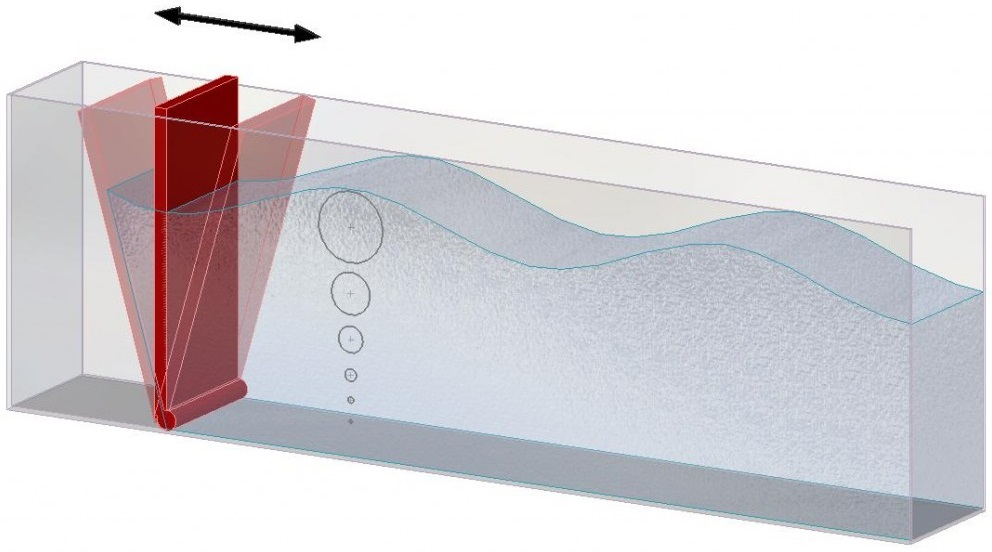
\includegraphics[height=3cm]{images/Wave_Maker(Flap).jpg}
        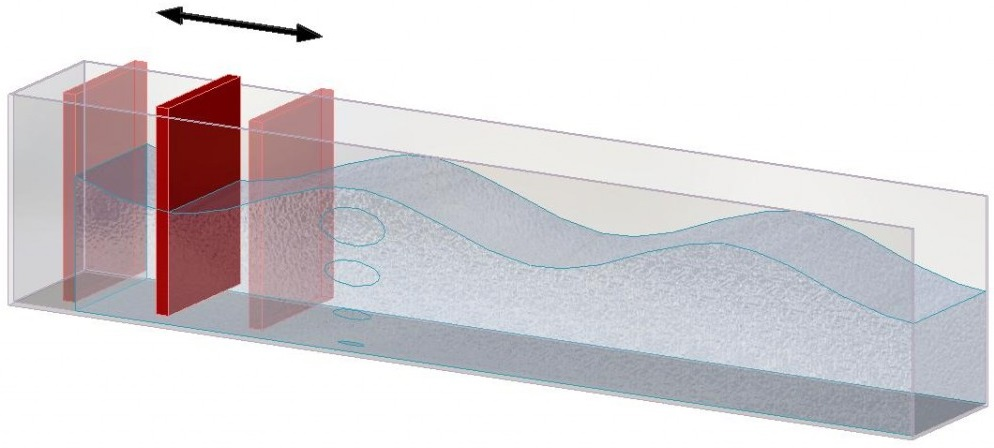
\includegraphics[height=3cm]{images/Wave_Maker(Piston).jpg}
    \end{center}
        \begin{tikzpicture} [remember picture, overlay]
            \node at (1.7, 1.0) {\scriptsize{(a) flap type}};
            \node at (7.6, 1.0) {\scriptsize{(b) piston type}};
        \end{tikzpicture}
        \caption{Various types of 2-dimensional wavemaker - (a) flap type (b) piston type}
        \label{Experimnet_System} 
\end{figure}

A piston-type wavemaker was built for the research, with the plate moving horizontally to push water. It can only generate 2-Dimensional waves, progressing in one direction; In fact, various types of waves (especially 3-Dimensional) can be generated if the plate has steps, each part moving in a certain sequence (It is called snake-like). Theoretically, the plate should move sinusoidally to generate sinusoidal waves. There is a range that the plate moves within, and it is called Stroke, denoted as $S_0$ hereinafter.

Previously, a small wavemaker was built for the former study, using a linear actuator of length 40$\mathrm{cm}$. It's a piston type, with an acrylic plate designed to fit in the wave channel. Both actuators and motor drivers utilize products of FUYU, Chengdu, but the wavemaker has the limitation of not being able to generate various waves. There is a controller, but it only changes the wave in several versions, without proper parameters that intermediate the generation of wave theoretically. To experiment successfully with models, certain conditions should be satisfied, based on model experiment principles such as Froude's law or Reynolds' law \cite{briggs2013basics, chakrabarti1994offshore}.

\subsection{Wavemaker theory}

Wavemaker theory investigates the properties and shapes of waves generated by the motion of the wavemaker within the wave channel. Fluids inside the tides must satisfy several principles of hydrodynamics and boundary conditions \cite{dean1991water, zhang2007deterministic}. Few differential equations and boundary conditions are derived from the geometry of the wave channel and the basic principle. The solution is the velocity potential, which gives the shape of the wave, its velocity, and other physical variables. It is expressed as a wave packet: the sum(superposition) of infinite waves of different wave numbers. The goal of the theory is to find out the relationship between the wave's shape and the plate's movement under the assumption that the plate moves sinusoidally.

\begin{figure}[h]
    \centering
    \captionsetup{}
    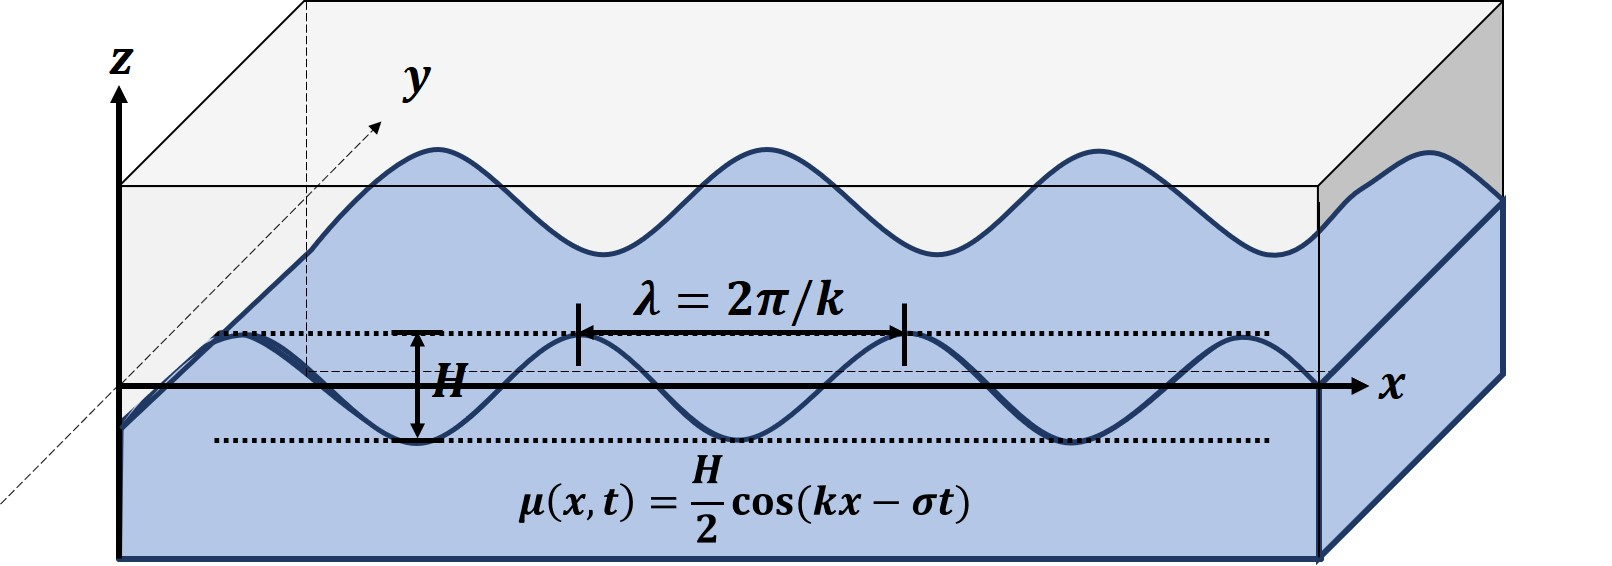
\includegraphics[width=13cm]{images/Water_Channel(Illustrated).jpg}
    \caption{Illustration of the wave channel}
    \label{Water_tank(Illustrated)}
\end{figure}

Several references start by inducing the Laplace equation about velocity potential. Before that, it should be guaranteed that the velocity potential can be defined. Let's begin with the continuity equation of mass. The Lagrangian differential for density $\rho$ is zero because the mass is conserved regardless of the type of fluid.
%
\begin{equation}
    {D\rho/Dt = d\rho/dt + \Vec{v} \cdot \nabla\rho = 0}\label{eq_001}
\end{equation}

$\rho$ is constant when the fluid is incompressible. Often, water is assumed to be incompressible, and it's not a major focus of the theory and experiment.

\begin{equation}
    {d\rho/dt = 0,~\nabla \cdot \vec{v} = 0}\label{eq_002}
\end{equation}

In a 2-Dimensional wave channel, fluid is irrotational: the curl of $\vec{v}$ is zero.
\begin{equation}
    {\nabla \times \vec{v} = 0}\label{eq_004}
\end{equation}

As a result, the potential function of the velocity field $\phi(x, z, t)$ can be defined and it satisfies the Laplace equation.

\begin{equation}
    \vec{v} = - \nabla \phi, ~\nabla^2 \phi = 
    \frac{\partial^2 \phi}{\partial x^2} + 
    \frac{\partial^2 \phi}{\partial z^2}\label{eq_005}
\end{equation}

$\phi(x, z, t)$ is a solution that meets several boundary conditions. By Kinematic Free-Surface boundary condition (denoted as KFSBC hereinafter), the shape of the free surface (water-air interface) $\eta(x, t)$ is expressed as:

\begin{equation}
    \eta = \frac{1}{g} \frac{\partial \phi}{\partial t}|_{z=0}\label{eq_007}
\end{equation}

Since $\eta$ is a displacement, it is related to $\phi$ by $v_{z}$ of the wave.
\begin{equation}
    -\frac{\partial \phi}{\partial z}|_{z=0} = \frac{\partial \eta}{\partial t}|_{z=0}\label{eq_008}
\end{equation}

$\eta$ is the shape of the wave, one of the main goals of wavemaker theory. Also, there are horizontal and vertical geometric boundary conditions:

\begin{enumerate}
    \item Vertically, the z-directional velocity at the bottom of the channel($z=-h$) should be zero.
    \begin{equation}
        \frac{\partial \phi}{\partial z}|_{z=-h} = 0\label{eq_009}
    \end{equation}

    \item Horizontally, there is a plate at one end of the channel. Denote the displacement of the plate as $S(z)$ (it is x-directional), and the boundary condition is expressed as:
    \begin{equation}
        F(x, ~z, ~t) = x - \frac{S(z)}{2} \sin{\sigma t} = 0\label{eq_010}
    \end{equation}

    This is one type of Kinematic boundary condition, and it must satisfy ${DF/Dt} = 0$. This condition can differ by the motion of the plate. The \textit{signal} for the wave plays its role here.
    \begin{equation}
        \frac{\partial F}{\partial t} = {\vec{v} \cdot \nabla F}\label{eq_011}
    \end{equation}

    \begin{equation}
        u - \frac{w}{2}\frac{\partial S}{\partial z}\sin{\sigma t} = \frac{S(z)}{2} \sigma \cos{\sigma t}\label{eq_012}
    \end{equation}

    With Taylor expansion, the boundary condition is derived by Taylor expanding Equation \ref{eq_012} at $x=0$.
    
    \begin{equation}
        u(0, ~z, ~t) = \frac{S(z)}{2} \sigma \cos{\sigma t} \label{eq_013}
    \end{equation}
    
\end{enumerate}

Solving Equation \ref{eq_005} with boundary condition, the solution is as follows:
\begin{equation}
    \phi(x, ~z, ~t) = A_p \cosh{k_p (h+z)} \sin{(k_p x - \sigma t)} + (Ax + B) + C \exp(-k_p x) \cos{k_s (h+z)} \cos{\sigma t}\label{eq_014}
\end{equation}

The first term represents the progressive wave, whereas the second term represents the free stream, which is generally zero. The third term represents a standing wave, with its amplitude decreasing exponentially. Especially, $k_s$ is the solution of the dispersion relation, which exists infinitely many.

Changing the form of Equation \ref{eq_008}:
\begin{equation}
    \frac{\partial \phi}{\partial z}|_{z=0} - \frac{\sigma^2 \phi}{g}|_{z=0} = 0\label{eq_015}
\end{equation}

\emph{Dispersion Relation}:
\begin{equation}
    \sigma^2 = gk_{p} \tanh{k_p h}\label{eq_016}
\end{equation}

Substituting Equation \ref{eq_016} with standing wave number $k_s$ gives:
\begin{equation}
    \sigma^2 = -gk_{s} \tan{k_s h}\label{eq_017}
\end{equation}

There are infinitely many solutions of Equation \ref{eq_017}, and let's denote the positive solution in the increasing order as $k_{s}(n)$: $k_{s}(1)$, $k_{s}(2)$, $k_{s}(3)$, ...\\
Expressing Equation \ref{eq_014} with linear combination with $k_{s}(n)$ as coefficients:
\begin{equation}
    \phi(x, ~z, ~t) = A_p \cosh{k_p (h+z)} \sin{(k_p x - \sigma t)} + \sum_{n=1}^{\infty} C_{n} \exp(-k_{s}(n) x) \cos{k_{s}(n) (h+z)} \cos{\sigma t}\label{eq_018}
\end{equation}

Again, the first term represents the progressive wave and the second term(linear combination) represents the standing wave decreasing exponentially. $k_s (n)$ is related to the damping coefficient of Equation \ref{eq_018} and the first mode has the smallest effect toward damping by $x$. Numerically, $k_s (1)$ exists between $\pi/2$ and $\pi$, and the amplitude of the mode decreases by the proportion of $exp(-k_s (1) x)$: 0.04 when $x=2h$, 0.009 when $x=3h$. For a long wave channel, the amplitude rapidly decreases. The length of the wave channel is $6m$ with water depth lower than $30cm$, which gives $x>20h$: The standing wave might be negligible.

Equation \ref{eq_018} must satisfy boundary condition - Equation \ref{eq_013}:
\begin{equation}
    u(0, ~z, ~t) = \frac{S(z)}{2} \sigma \cos{\sigma t} = - \frac{\partial \phi}{\partial x}|_{x=0}\label{eq_019}
\end{equation}
\begin{equation}
    \frac{S(z)}{2} \sigma = - A_p k_p \cosh{k_p (h+z)} + \sum_{n=1}^{\infty} C_n k_s (n) \cos{k_s (n) (h+z)}\label{eq_020}
\end{equation}

In the case of the research, $S(z)$ is constant: $S(z) = S_0$. It's the simplest form of \textit{Piston type Wavemaker}. Also, coefficients from Equation \ref{eq_020} can be derived from orthogonality. With all this information, the shape of the wave is:
\begin{equation}
    \eta(x, t) = \frac{A_p \sigma}{g}\cosh{k_p h} \cos{(k_p x - \sigma t)} + \sin{\sigma t} \sum_{n=1}^{\infty} \frac{\sigma C_n}{g} \exp{(-k_s (n) x)} \cos{(k_s (n) h)}
    \label{eq_021}
\end{equation}

Similar to Equation \ref{eq_014} and Equation \ref{eq_018}, the first term represents a progressive wave and the second term represents standing waves, decreasing exponentially. As discussed earlier, the standing waves are negligible and the wave height $H$ can be expressed by linearly approximating each eigenfunction.
\begin{equation}
        H = \frac{4 S_0 \sinh{kh}}{\sinh{2kh} + 2kh}(\sinh{k(z_d - h)} - \sinh{k(z_u - h)})\label{eq_022}
\end{equation}

From Equation \ref{eq_022}, $k$ is the wave number formerly given($k_p$), and $z_u$, $z_d$ denotes the depth of the plate, each corresponding to the upper part and the bottom part, respectively. If the plate exists throughout the depth, $S(z) = S_0$, $z_d = h$, and $z_u = 0$. Wave height and the wave function are expressed as:
\begin{equation}
    \eta(x, ~t) = \frac{H}{2} \cos{(kx-\sigma t)}, ~H = \frac{4 S_0 \sinh^2 {kh}}{\sinh{2kh} + 2kh} = \frac{4 S_0 \sinh^2 {z}}{\sinh{2z} + 2z}~(z=kh)
    \label{eq_023}
\end{equation}

From Equation \ref{eq_023}, several numbers such as \emph{Stroke} $S_0$ and depth of the water $h$ can be regulated externally. Also, wave number $k$ and angular frequency $\omega$ are related by dispersion relation (Equation \ref{eq_016}), so only $k$ or $\omega$ is needed to be set with proper structural conditions.

This theory has been expanded with a lot of approximations of boundary conditions and calculations. $H/h$ and $H/\lambda$ should be small enough for it, and on other occasions, nonlinear theories like Stokes Nonlinear Wave Theory and Cnoidal Wave Theory are needed. In a special case, a tsunami is generated by Solitary Wave Theory \cite{madsen1970waves, watts1998wavemaker, fenton1990nonlinear}.

\subsection{Wave absorber}

As the wave is generated by the wavemaker, it progresses inside the tank and is divided into progressive waves and reflected waves reflected by the surrounding obstacles, such as walls or other coastal models. According to the principle of superposition, the surface wave is expressed as a linear combination of the progressive wave and the normal wave by reflection, and the normal wave is the main cause of the error from an experiment. A wave absorber is a device that prevents or extinguishes these reflected waves: Generally, they are divided into active and passive types \cite{ouellet1986survey}.

The active absorber is another wavemaker, but it should generate a new wave to completely offset the incident wave. It requires abilities to measure the incident wave and generate the proper wave immediately, by moving the plate. It is fairly expensive equipment and has limited use since it is designed to use in specific environments. This method is to install another wavemaker near the wall where the incident wave collides, and the wavemaker controls its motion to generate the wave that offsets the reflected wave. This is called the "Absorbing Wavemaker", and it should be possible to measure the shape of the wave by the plate and to perform overlapping motion accordingly \cite{frigaard1995absorbing}. The reflection coefficient can be significantly reduced, but its usability is not as wide as a passive wave absorber.

The passive wave absorber aims to minimize the energy of the reflected wave by installing an additional structure. Unlike active absorbers, it is impossible to completely extinguish reflective waves for passive ones, no matter how optimized they are. Also, there are various structures such as horsehair, crushed rock, etc. In particular, porous structures are used to effectively extinguish waves, and many studies have been conducted on it, such as a comparison of reflection coefficients according to porosity, and their efficiency has already been proven. In addition, ramps are also used to minimize reflective waves in 3-Dimensional waves, in areas that researchers are not interested in. It was found that the convex parabolic surface had the lowest reflection coefficient.

\subsection{Froude Similarity Law}

Physical features change as the dimension of the physical system changes. The scale factor between the real system and the experimental model is needed, and the Froude Similarity Law is held \cite{briggs2013basics, chakrabarti1994offshore}.
\begin{equation}
    Fr_{1} = Fr_{2}, ~Fr = \frac{V}{\sqrt{gL}}
    \label{froude number}
\end{equation}

$V$ is the velocity of the moving element, $L$ is the characteristic length of the system, and $g$ is the gravitational acceleration. There are other dimensionless numbers such as the Prantdl number, Reynolds number, etc. but the gravitational effect is dominant rather than the viscosity of the fluid or diffusion.

The moving element of both systems 1 and 2 (which is wave channel and open sea, respectively) is water(wave), so the Froude number is expressed as equation \ref{froude number of wave} with a dispersion relation.

\begin{equation}
    Fr_i = \sqrt{\frac{\tanh{k_i h_i}}{k_i L_i}}
    \label{froude number of wave}
\end{equation}

\begin{enumerate}
    \item System1: Wave Channel
    
    It is known that the characteristic length of the channel with a rectangular cross-section is $L_2 = \frac{2ah_1}{a+h_1}$, where $a$ and $h_1$ correspond to the width and depth of the channel, respectively.
    \begin{equation}
        Fr_1 = \sqrt{\frac{\tanh{k_1 h_1}}{k_1 h_1} \times \frac{a+h_1}{2a}}
    \end{equation}
    
    \item System2: Open Sea
    
    There are no references to the characteristic length of the open sea. It's assumed that the open sea is a large rectangular channel with $h_2 \gg\ a$, which gives $L_{2} = 2h_{2}$, where $h_2$ is the depth of the water.
    \begin{equation}
        Fr_2 = \sqrt{\frac{\tanh{k_2 h_2}}{k_2 h_2} \times \frac{1}{2}}
    \end{equation}
\end{enumerate}

Froude numbers of both systems agree:
\begin{equation}
    \frac{a+h_1}{2a} f(z_{1})  = f(z_{2})
    \label{froude number equation}
\end{equation}

where $f(x) = \frac{\tanh{x}}{x}$ and $z_i = k_i h_i$. The experiment condition was set as $a = 0.30m$, $h_{1} = 0.15m$. Also, the wave is categorized by $h/\lambda < 1/20$ (long wave) and $h/\lambda > 1/2$ (short wave). With these constants, Equation \ref{froude number equation} gives numerical solutions: $\omega \sim \pi$ for the long wave and $\omega \sim 4\pi$ for the short wave. In the case of a sinusoidal wave, $\omega \sim 4\pi$.

%%%%%%%%%%%%%%%%%%%%%%%%%%%%%%%%%%%%%%%%%%%%%%%%%%%%%%%%%%%
% \section{Theoretical Background}

% \subsection{Wave Channel}

% A wave channel is a tank that creates a small environment to reproduce phenomena occurring on the coast or in the open sea. Its size and shape vary by usage, from small rectangular tanks to long and wide square tanks. The one at the school has a length of 6,m, a width of 30, cm, and a height of 40, cm. The 3-Dimensional wave tank is the most popular since it's suitable for using a wave maker that generates 3-Dimensional waves. The "3-Dimensional" means that the wave is generated with vortexes: the fluid is rotational ($\nabla \times \vec{v} \neq 0$). On the other hand, "2-Dimensional" means that the wave is generated without vortexes: if the wave channel is rectangular and the waves progress along the side, there is no perpendicular fluid movement.

% Previously, a small rectangular parallelepiped wave tank with dimensions of length 6,m, width 30, cm, and height 40, cm was built and utilized. It is constituted of 2 modules, each with a length of 2,m, and they were connected and sealed to prevent water leakage. The frame is made of aluminum profile, and the walls are made of transparent acrylic plates (5, T: 5, mm thick). Also, there are wheels at the bottom for mobility, height adjustment, and horizontal adjustment. It was mainly built to test the Masonry structure of breakwater, but it could be used to test the stability of a ship or the durability of a coastal structure, providing an appropriate environment.

% \subsection{Wave Maker}

% A wave maker is a device that generates waves in a wave channel. It is usually categorized by the movement of the plate. In general, there are piston types, plunger types, flap types, etc.

% \begin{figure}[H]
% \centering
% \captionsetup{justification=centering}
% 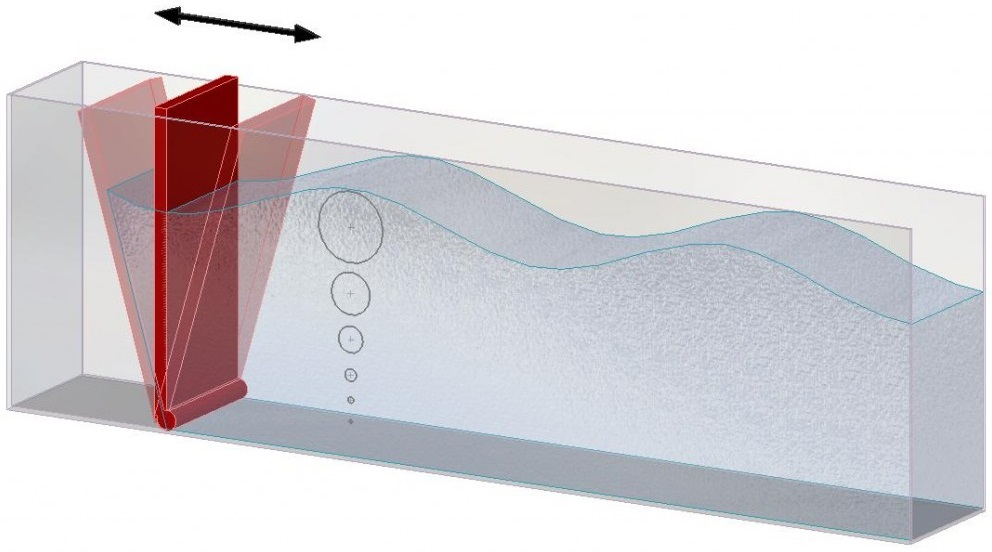
\includegraphics[height=3cm]{images/Wave_Maker(Flap).jpg}
% 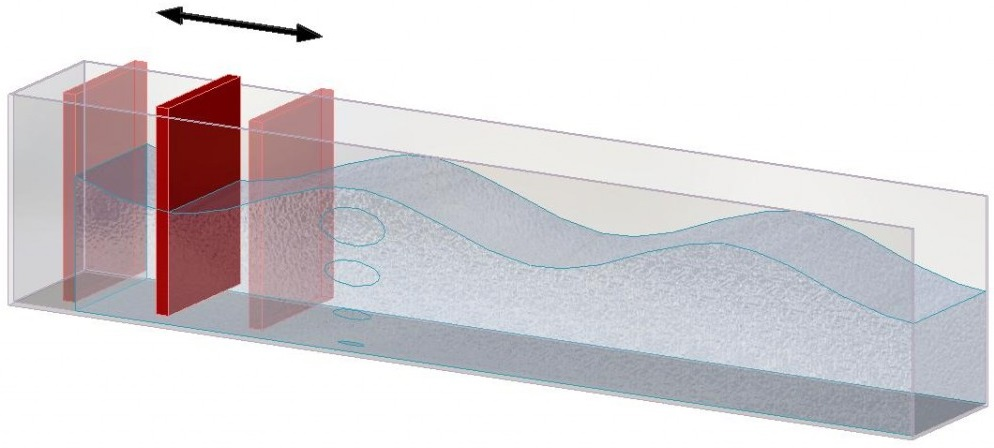
\includegraphics[height=3cm]{images/Wave_Maker(Piston).jpg}
% \caption{Flap type (left) and Piston type (right) wave maker}
% \label{various types of wave makers}
% \end{figure}

% A piston type was built for this research, with each element (part) of the plate moving horizontally to push water. The plate is not separated by each part: it moves as a single, integrated body. It can only generate 2-Dimensional waves, progressing in one direction. Various types of waves (especially 3-Dimensional) can be generated if the plate has steps, and each part moves in a certain sequence (referred to as \textit{snake-like}). Theoretically, the plate should move sinusoidally to generate sinusoidal waves. There is a range that the plate moves within, and it is called \textit{Stroke}, denoted as $S_0$ hereinafter.

% Previously, a small wave maker was built for the former study, using a 40, cm long linear actuator. It is a piston type, with an acrylic plate that is designed to fit the size of the tank. Both actuators and motor drivers utilize products of \textit{FUYU, Chengdu}, but the wave maker has the disadvantage of not being able to generate various waves. There is a controller, but it only changes the wave in several versions, without proper parameters that intermediate the generation of waves. It cannot control the phase velocity or wave height. Therefore, the wave generator for this research needs to be improved.

% \subsection{Wave Parameters}

% There are various parameters used to describe waves. Some of the important ones are:

% \begin{itemize}
% \item Wave Height ($H$): The vertical distance between the crest and trough of a wave.
% \item Wave Length ($L$): The horizontal distance between two successive crests or troughs of a wave.
% \item Wave Period ($T$): The time taken for a wave crest to travel a distance equal to one wavelength.
% \item Wave Number ($k$): The spatial frequency of the wave, defined as $k = \frac{2\pi}{L}$.
% \item Phase Velocity ($C$): The speed at which a specific phase of the wave (e.g., crest) moves in a particular direction.
% \item Group Velocity ($C_g$): The speed at which the energy of a wave group (composed of multiple waves) propagates.
% \end{itemize}

% These parameters play a crucial role in characterizing the behavior and properties of waves.

% \subsection{Wave Absorption}

% In a wave channel, wave absorption is necessary to prevent the reflection of waves from the boundaries of the tank, which could interfere with the desired wave patterns. Different techniques can be employed for wave absorption, such as:

% \begin{itemize}
% \item Sloping Beach: The tank bottom is inclined towards the wave-maker end, allowing the waves to dissipate their energy as they reach the boundary.
% \item Porous Structures: Placing porous materials at the tank boundaries to absorb and dissipate the energy of the waves.
% \item Wave Dissipators: Installing specialized structures, such as perforated plates or wave absorbers, to dampen the wave energy and prevent reflection.
% \end{itemize}

% The choice of wave absorption technique depends on the specific requirements of the experiment or simulation being conducted in the wave channel.

% \subsection{Wave Measurement}

% To analyze and study wave behavior in the wave channel, various measurement techniques can be employed, including:

% \begin{itemize}
% \item Wave Gauges: Sensors placed in the tank to measure the water surface elevation and obtain wave height and wave period data.
% \item Laser Doppler Vibrometry: Using laser beams to measure the velocity of the water particles and obtain information about wave characteristics.
% \item Video Analysis: Recording videos of the waves and analyzing them using image processing techniques to extract wave parameters.
% \end{itemize}

% These measurement techniques enable researchers to gather quantitative data about the waves generated in the wave channel.

% In conclusion, the wave channel and wave maker provide a controlled environment for studying wave phenomena. Understanding wave parameters, absorption techniques, and measurement methods is crucial for conducting accurate experiments and simulations in the wave channel.

 % 이론적 배경
        %Text Check!
\section{Method}

\subsection{Wave Channel}

The extension of the water tank was necessary since the original channel was too short for the new wavemaker. Also, additional devices such as a coastal model and a wave absorber were built. It will be discussed in this section.

\subsubsection{Wave Channel Extension}%Check!

The wave channel was extended to $6,000\mathrm{~mm}$ to get extra space for the coastal model, wavemaker, and a domain for wave generation. A new module was built similarly, with the framework of the aluminum profile 3030 series (cross-sectional area $30\mathrm{~mm} \times 30\mathrm{~mm}$) and the inner wall of an acrylic plate ($5\mathrm{~mm}$ thickness), with its dimension $2,000\mathrm{~mㅡ}$ $\times$ $300\mathrm{~mm}$ $\times$ $400\mathrm{~mm}$. It was inserted in the middle of the other two.

The wave channel needed sealing between the modules to prevent water leakage. Silicone pads were cut into U-shapes so that they fit right into the section where the aluminum profile meets. Also, acrylic rods were attached to each side of the modules and long bolts passed through them, tightening the link and pressing silicone pads.


\begin{figure}[H]
    \begin{center}
        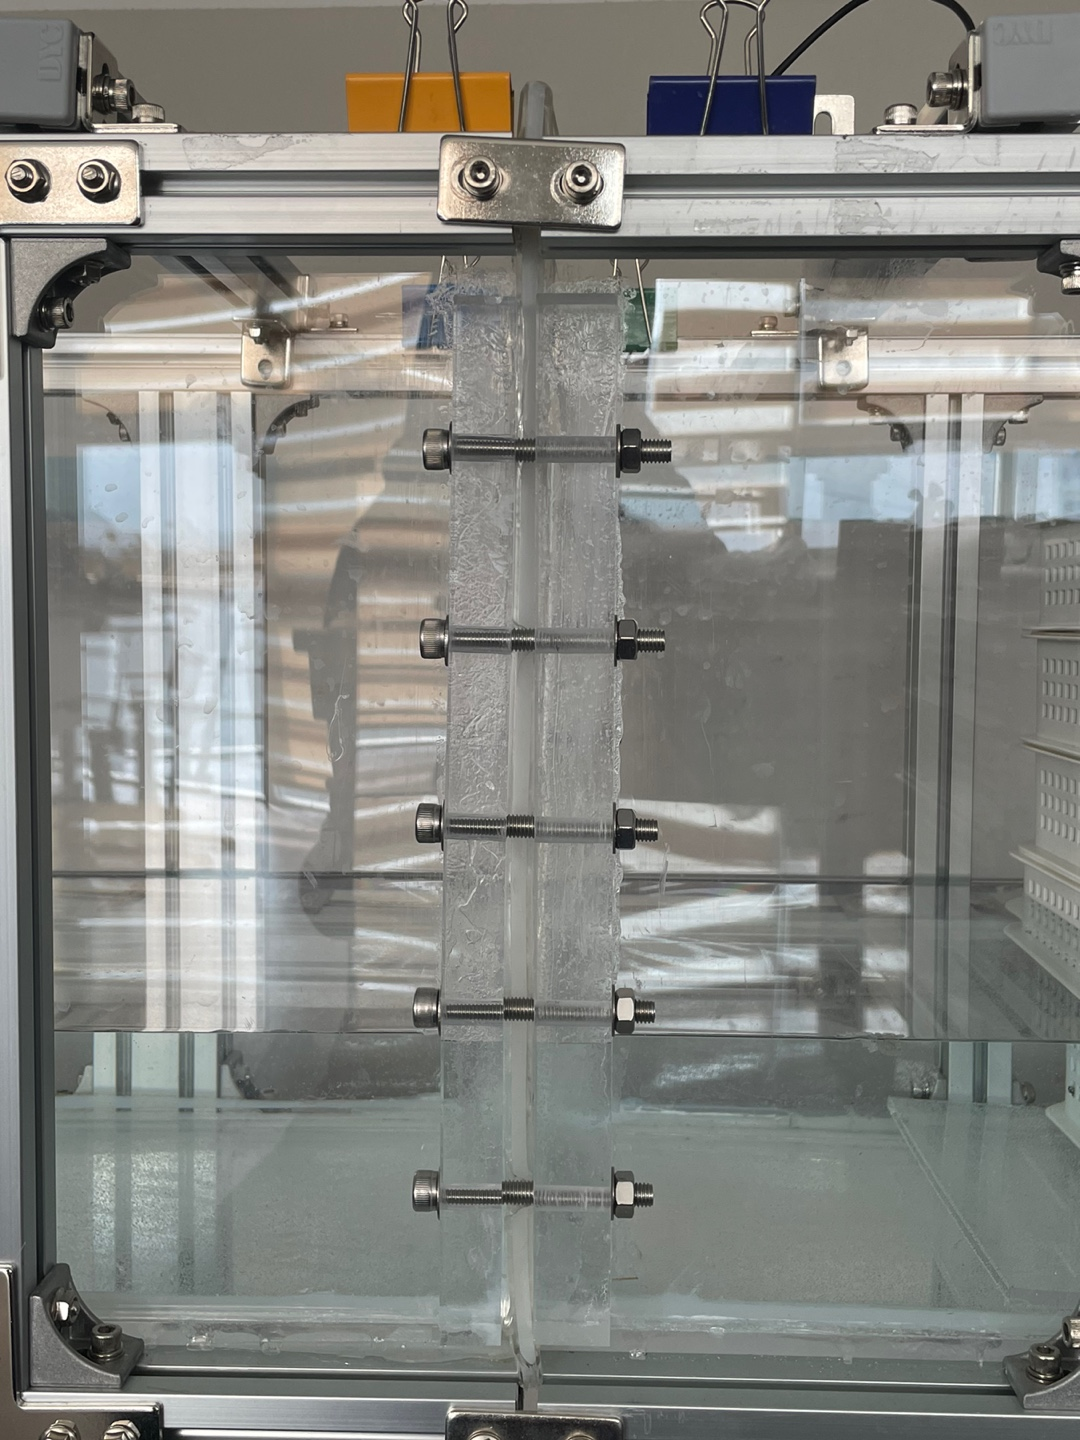
\includegraphics[height=5cm]{images/Connection(Side).jpg}
        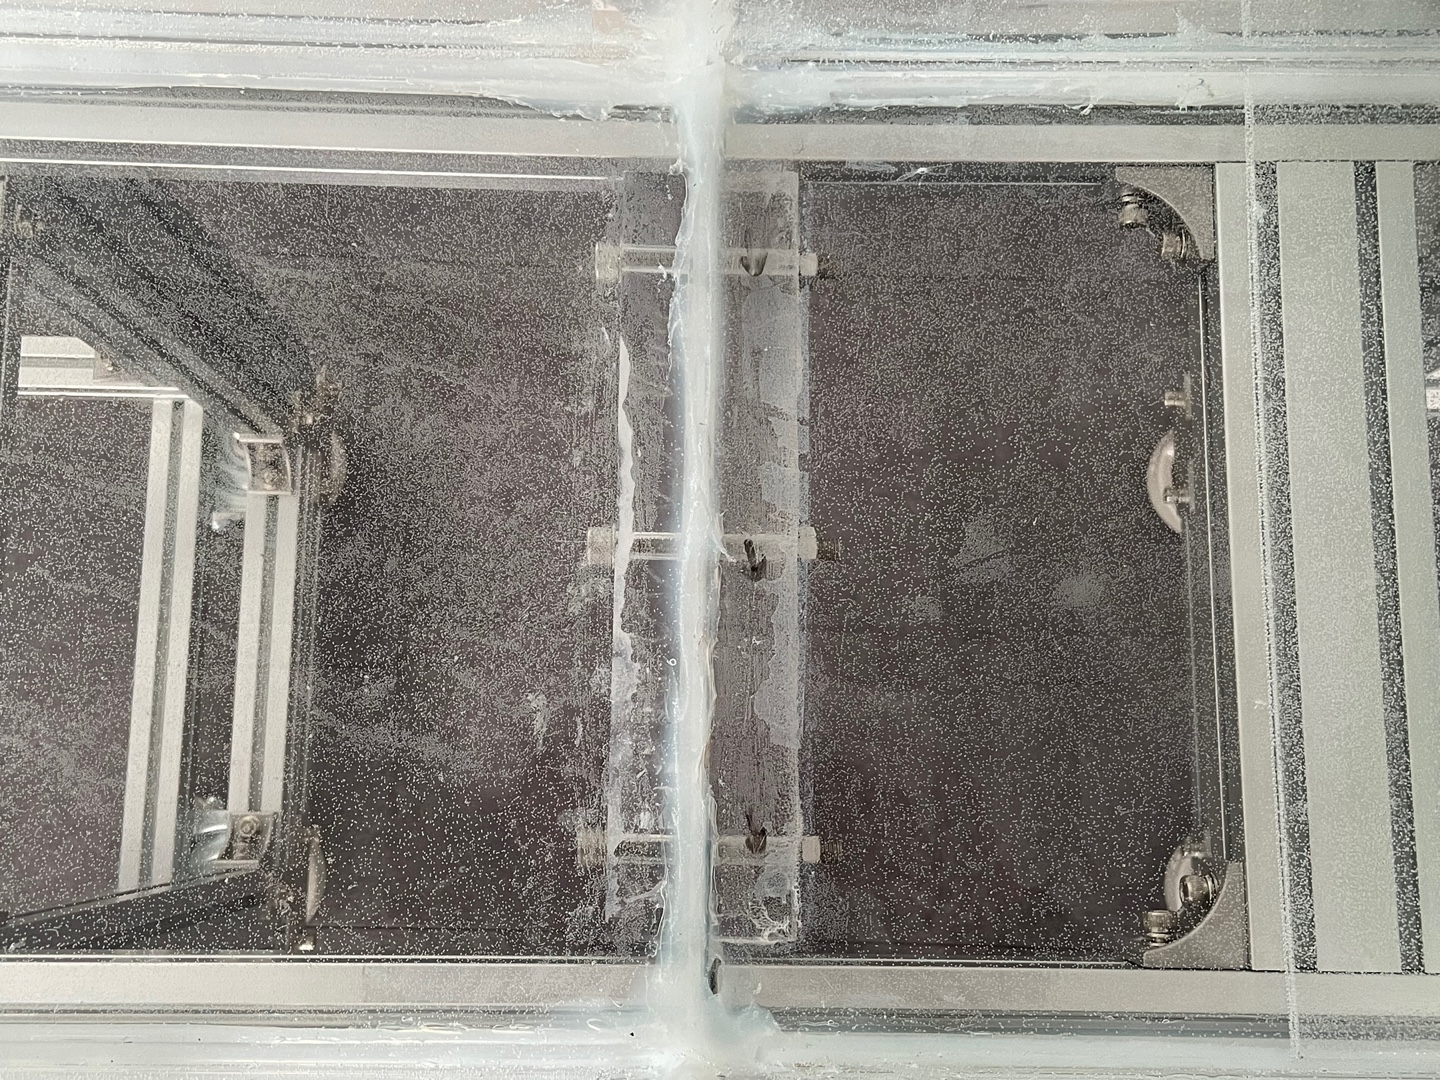
\includegraphics[height=5cm]{images/Connection(Silicone).jpg}
    \end{center}
        \begin{tikzpicture} [remember picture, overlay]
            \node at (2.1, 0.6) {\scriptsize{(a)}};
            \node at (6.0, 0.6) {\scriptsize{(b)}};
        \end{tikzpicture}
        \caption{Connection of the modules - (a) side (b) bottom}
        \label{connection} 
\end{figure}

Lastly, smaller gaps were sealed with a silicone gun. Smaller gaps were spotted from the water leakage when water was poured. After a few trial-and-error, the wave tank was sealed completely (Figure \ref{wave channel}). Also, the entire tank must be straight and flat overall. All three modules needed to be aligned straight. There are four wheels at the bottom of each module with a screw so that the height can be adjusted by tightening it.

\begin{figure}[H]
    \centering
    %\captionsetup{justification=centering}
    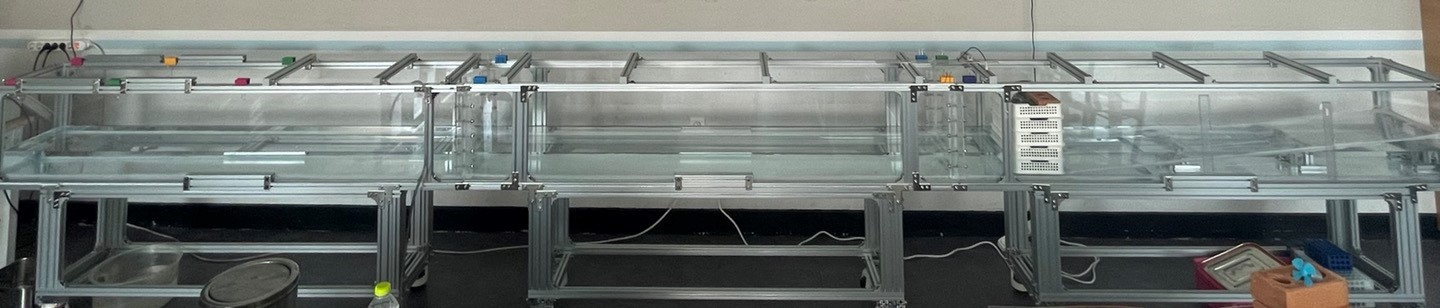
\includegraphics[width=\textwidth]{images/Wave_Tank(without_Generator).jpg}
    \caption{Wave channel}
    \label{wave channel}
\end{figure}

\subsubsection{Wave Absorber}%Check!

As the plate moves back and forth, waves that do not go in the direction of the coastal model must be extinguished to reduce systematic error. These waves could interfere in a region behind the wavemaker, exerting force on the plate. There is an existing wave absorber, a rectangular parallelepiped with holes in a three-dimensional grid printed with a 3D printer. The holes were not completely perforated but filled with wires and they effectively extinguish the wave.

According to previous studies, the wave absorber that can be made and installed to the wave channel in the lab is a rectangular parallelepiped brick of a porous structure like the previous one. Based on this idea, the prototype was made with a stainless steel box, with holes drilled through. But it was too difficult to handle and the box was void: Not proper to play the role. Thus, the baskets with holes were used, filled with scrubbers. The baskets fit in the wave channel, stacked into five floors. There is a way to test the ability of a wave absorber, but generating a proper sinusoidal wave is before it.

\begin{figure}[H]
    \begin{center}
        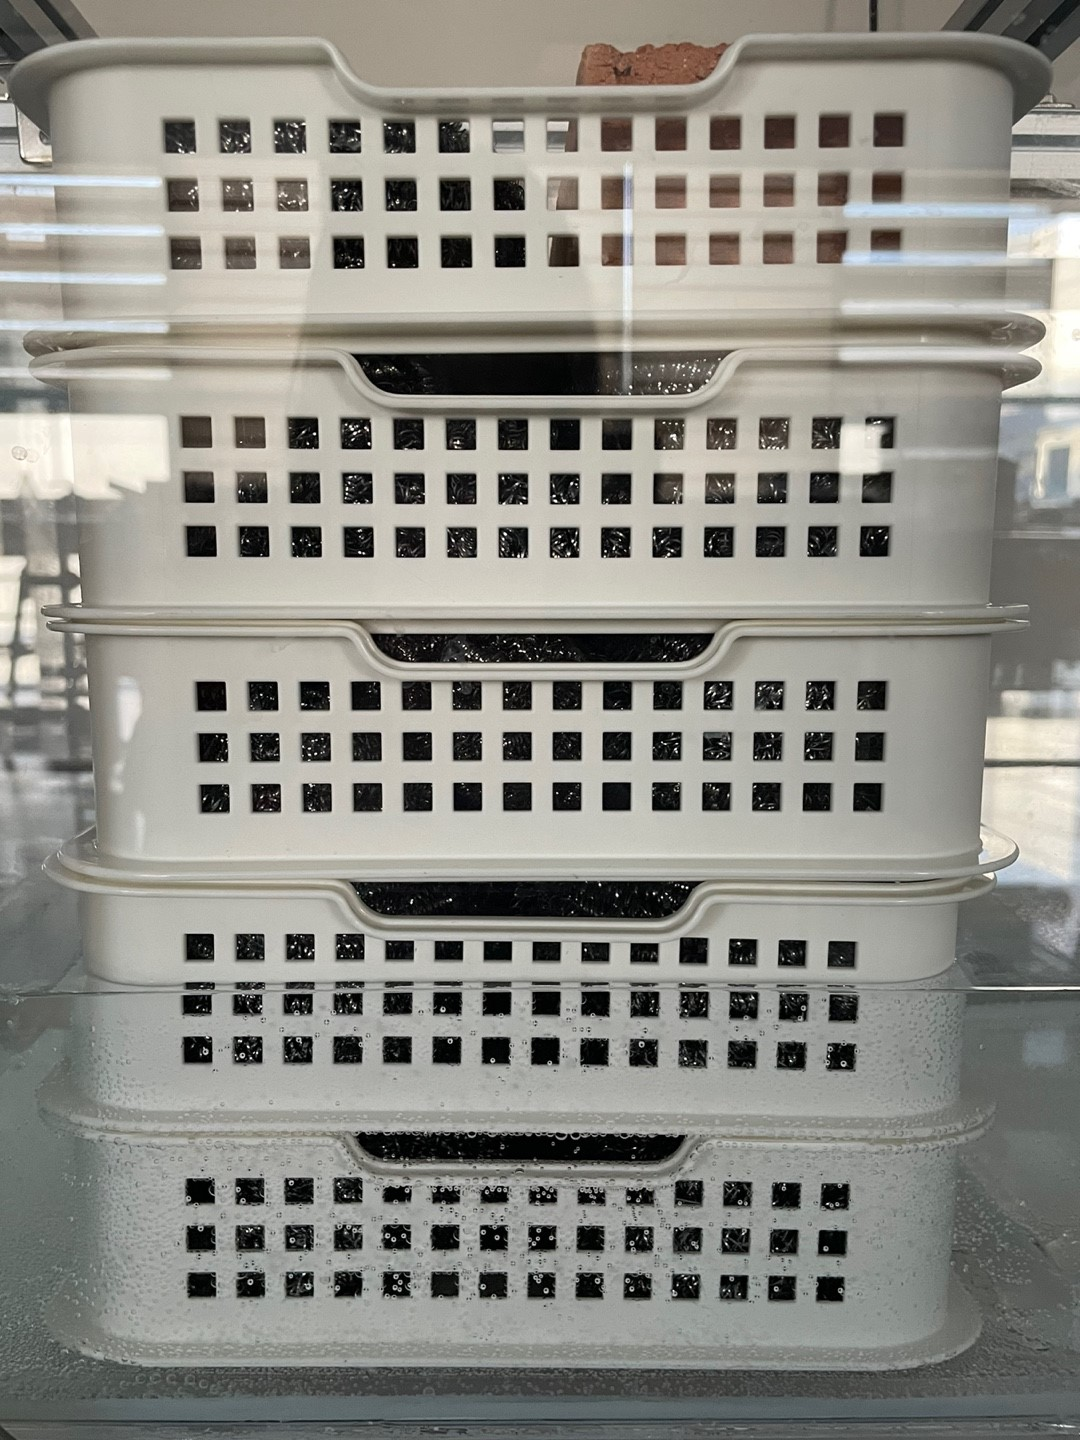
\includegraphics[width=5cm]{images/Wave_Absorber(Side).jpg}
        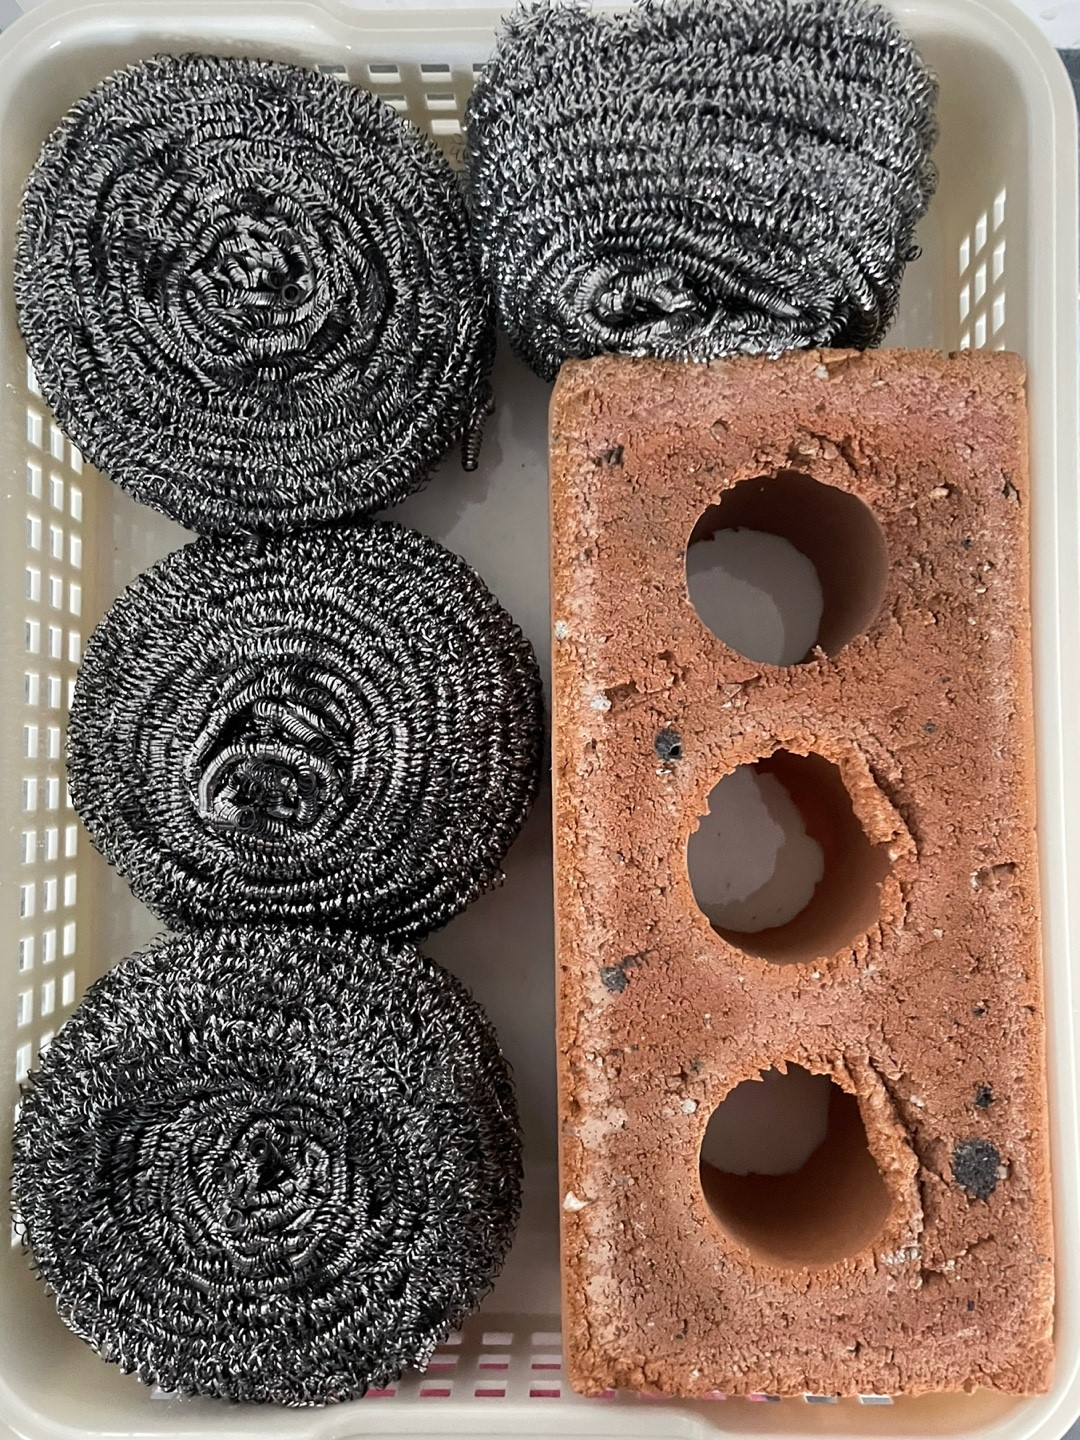
\includegraphics[width=5cm]{images/Wave_Absorber(Top).jpg}
    \end{center}
        \begin{tikzpicture} [remember picture, overlay]
            \node at (2.3, 0.6) {\scriptsize{(a)}};
            \node at (7.5, 0.6) {\scriptsize{(b)}};
        \end{tikzpicture}
        \caption{Wave absorber - (a) side (b) top}
        \label{Experimnet_System} 
\end{figure}

\subsubsection{Coastal Model}%Check!

A ramp was made as the coastal model. It would depend on the experiment, but the actual underwater terrain should have a slope from the seabed to the coast. Extra spaces could be provided at the end of the coast, allowing structures to be installed on flat land. Only the ramp was installed with the slope of $1/10$, considering that $1/20$ or $1/10$ is appropriate. Regarding that tank is $6,000\mathrm{mm}$ long and $400\mathrm{mm}$ high, the dimension was set as the length of $2,000\mathrm{m}$ and the height of $200\mathrm{mm}$. Bur for conducting the experiment verifying the generated wave, it needs to be detached.

An acrylic plate with a thickness of $5\mathrm{mm}$ was supported below with pedestals in three steps, made of aluminum profile bars. These pedestals were also detachable (Figure \ref{Coastal_Model(Ramp)}).

\begin{figure}[H]
    \centering
    %\captionsetup{justification=centering}
    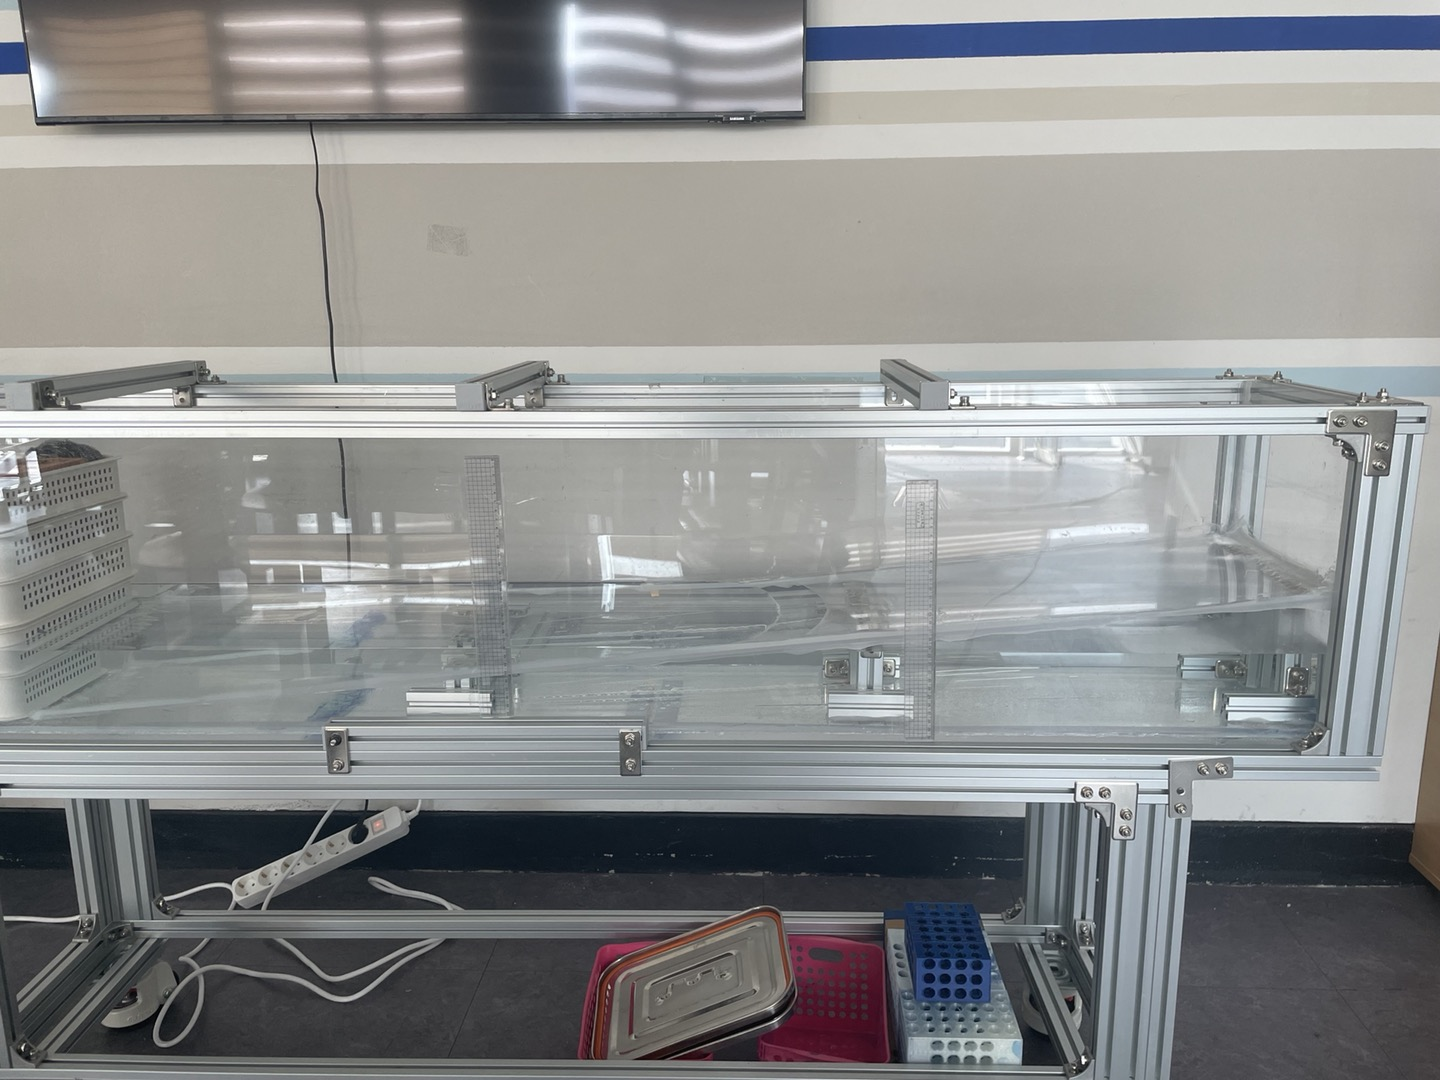
\includegraphics[width=11cm]{images/Coastal_Model(Ramp).jpg}
    \caption{Coastal Model - Ramp}
    \label{Coastal_Model(Ramp)}
\end{figure}

\subsection{Wavemaker}%Check!

The wavemaker consists of a driving unit and a control unit. The driving unit is a mechanical part of the wavemaker that moves the motor, and it is composed of a linear actuator and several structural components. The control unit is a circuit consisting of a motor driver, a Teensy3.2, a transformer, and other circuit diodes and it executes the code.

\begin{figure}[H]
    \centering
    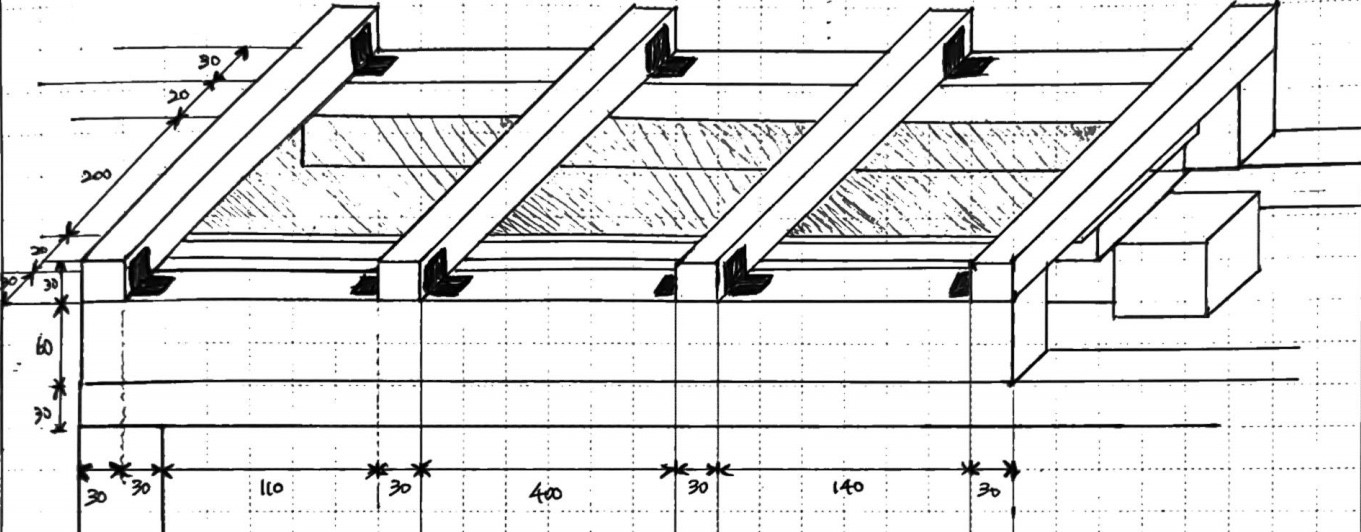
\includegraphics[width=12cm]{images/Wave_Maker(Design_not_drawn_to_scale).jpg}
    
    \caption{The design of the wave channel (Not drawn to scale)}
    \label{Wave_Tank(Design)}
\end{figure}

\subsubsection{Driving Unit}

A main component of the driving unit is a linear actuator, which converts the rotating motion of the motor to translating motion of an object through the screw thread (Figure \ref{linear actuator} The product is the FSK80 series from FUYU, Chengdu. Here is the basic information about the linear actuator.

\begin{table}[H]
    \centering
    \captionsetup{justification=centering}
    \begin{tabular}{l|l}
        \hline
        guide width $(\mathrm{mm})$                       & 80                                     \\
        repeat position accuracy $(\mathrm{mm})$          & +-0.02                                 \\
        motor                                  & stepper 60102                          \\
        rail model                             & dual rail W12 $\times$ H8              \\
        ball screw model                       & 16                                     \\
        \textbf{stroke $(\mathrm{mm})$}                  & \textbf{50 - 1000}                                    \\
        pitch                                  & 10                                     \\
        \textbf{horizontal full payload speed $(\mathrm{mm/s})$}   & \textbf{230}                                    \\
        vertical full payload speed $\mathrm{(mm/s)}$     & 60                                     \\
        side mounting payload speed $\mathrm{(mm/s)}$     & 210                                    \\
        \textbf{rated horizontal payload $\mathrm{(kg)}$}          & \textbf{40}                                     \\
        rated vertical payload $(kg)$            & 20                                     \\
        rated side mounting payload $(kg)$       & 15                                     \\
        noisy without payload $(db)$             & 79                                     \\
        rated payload noisy $(db)$               & 70                                     \\
        \textbf{acceleration $(mm/s^{2})$} & \textbf{500}                                    \\ \hline
    \end{tabular}%
    \caption{Specification of linear actuator - \textit{FSK80} Series}
    \label{specifiacion of linear actuator}
\end{table}

An $80\mathrm{~cm}$ long linear actuator was used. It is attached to an aluminum board and frameworks (Figure \ref{Wave_Tank(Design)}). The framework consists of an aluminum profile 3030 series. The linear actuator can bear up to $40\mathrm{~kg}$ horizontally, and its maximum speed is $230\mathrm{mm/s}$ with a full payload. The acceleration of the object is $500\mathrm{mm/s^{2}}$.

Limit switches were used to indicate the end of the actuator and the moving range of the motor. It's a sensor that sends out different voltage signals when metal is detected on one side of it (Figure \ref{limit switch}). 2 pieces were used, one at each end of the rail. As the object (the one moving through the rail) passes the switch, metal is detected and the location - angular displacement - is checked to limit the range of the motion.

\begin{figure}[H]
    \begin{center}
        \scalebox{-1}[1]{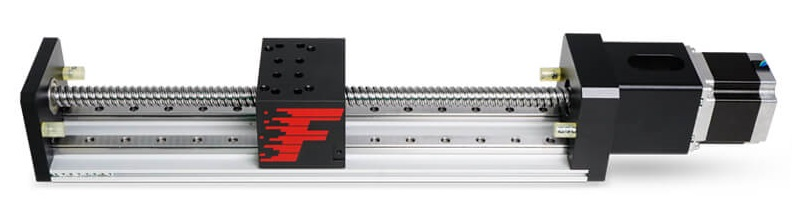
\includegraphics[width = 12cm]{images/Linear_Actuator.jpg}}
        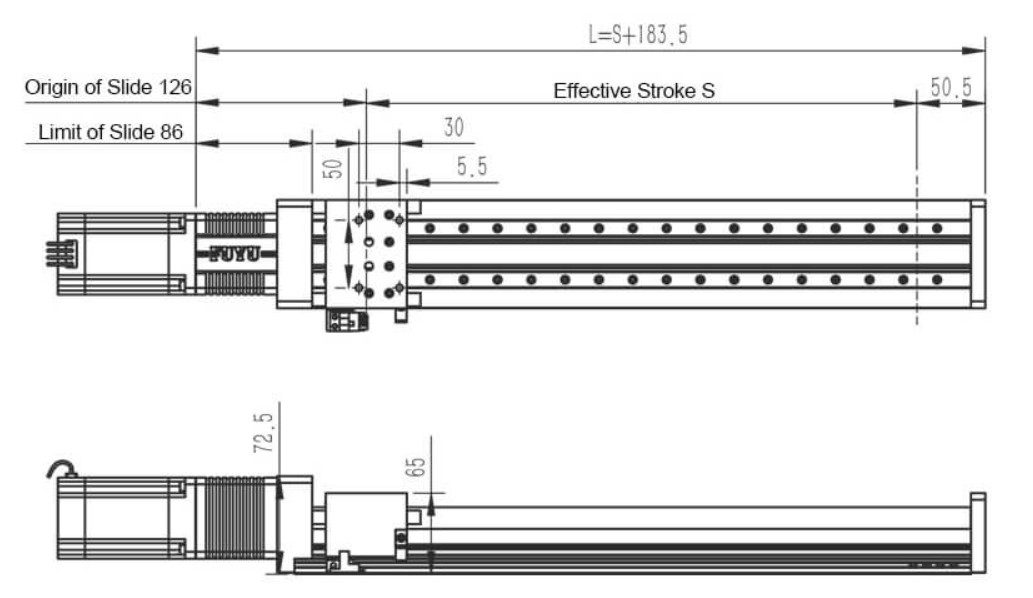
\includegraphics[width = 12cm]{images/Linear_Actuator(Design).jpg}
    \end{center}
        \begin{tikzpicture} [remember picture, overlay]
        \node at (2.0, 11.0) {(a)};
        \node at (2.0, 7.6) {(b)}; %1.1
        \end{tikzpicture}	
        \caption{Linear actuator - (a) \textit{FSK80} series (b) Design}
        \label{linear actuator}
\end{figure}

\begin{figure}[H]
    \centering
    \captionsetup{justification=centering}
    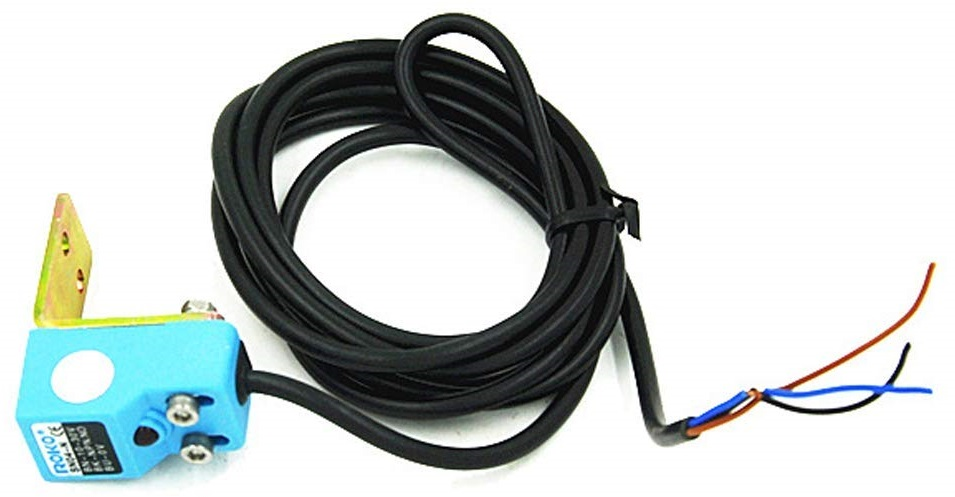
\includegraphics[width = 6cm]{images/Limit_Switch.jpg}
    \caption{Limit Switch}
    \label{limit switch}
\end{figure}

\subsubsection{Control Unit}

The control unit consists of Teensy 3.2, DRV8825, Microstep Driver (ST-M5045), and $24\mathrm{~V}$ SMPS. Teensy 3.2 is a main CPU board and executes the inserted code (Figure \ref{Teensy3.2}). For further information, refer to www.pjrc.com/teensy.

\begin{figure}[H]
    \centering
    \captionsetup{justification=centering}
    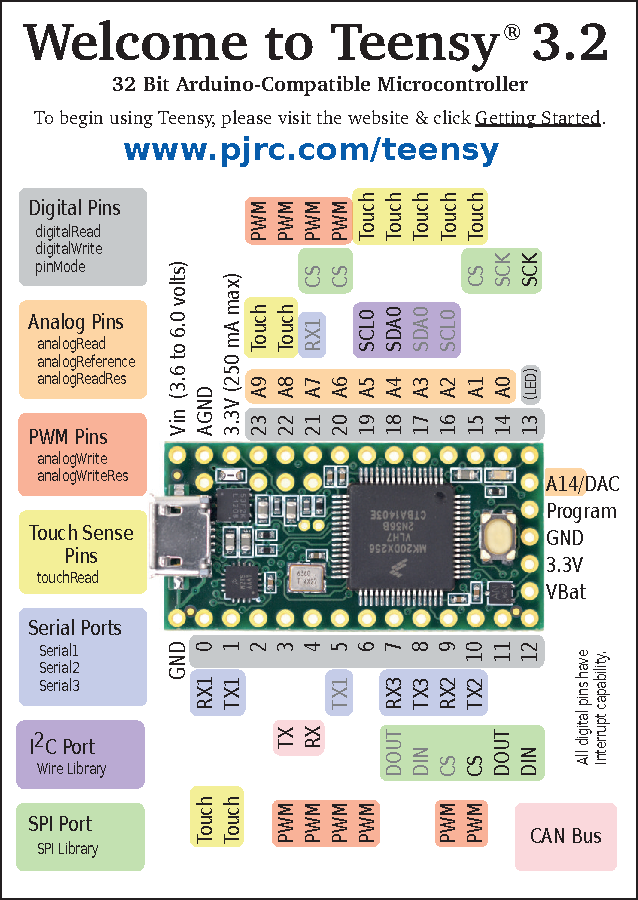
\includegraphics[width=6cm]{images/Teensy3.2 - 1.pdf}
    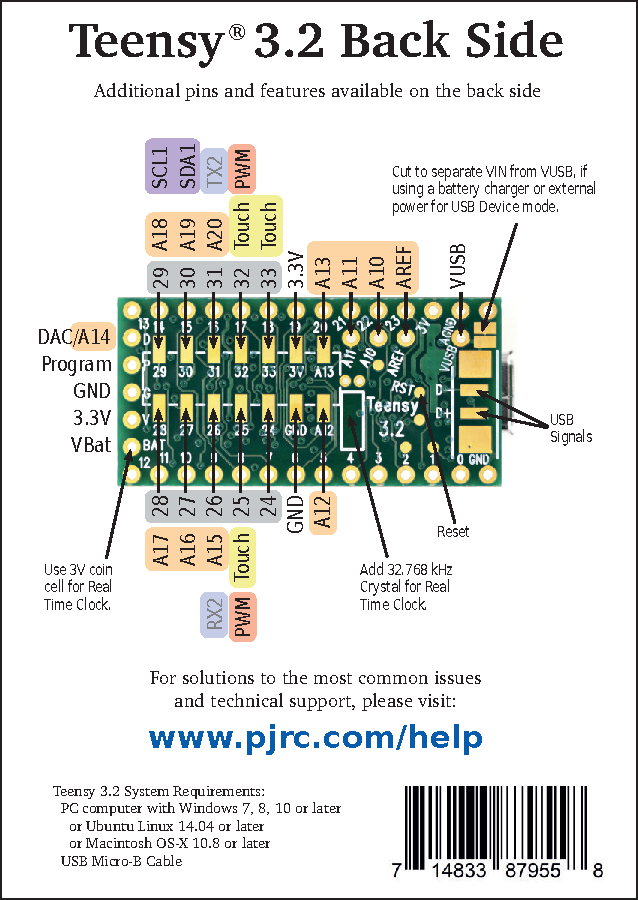
\includegraphics[width=6cm]{images/Teensy3.2 - 2.pdf}
    \caption{Pin map of Teensy 3.2}
    \label{Teensy3.2}
\end{figure}

It needs $3.2\mathrm{~V}$ of power supply and uses Teensyduino for coding, which is a software add-on for the Arduino to run sketches on the Teensy. The basic information is shown below (Table \ref{Specification of Teensy 3.2}). Overall, the Teensy board can communicate faster than other Arduino boards.

% it's one of the revised versions of \textit{Arduino} for use in \textit{Teensy3.2}. IDE is the same as \emph{Arduino}, but the compiler is different since \textit{Teensy} is not compatible with \textit{Uno, Nano}, and other Arduino boards. Here is the basic information:

% https://www.pjrc.com/teensy/teensyduino.html

 \begin{table}[H]
     \centering
     \begin{tabular}{l}
        \hline
        ARM Cortex-M4 at 72 MHz\\
        256K Flash, 64K RAM, 2K EEPROM\\
        \textbf{USB device 12 Mbit/sec}\\
        34 digital input/output pins, 12 PWM output pins\\
        21 analog input pins, 1 analog output pin, 12 capacitive sense pins\\
        3 serial, 1 SPI, 2 I2C ports\\
        1 I2S/TDM digital audio port\\
        1 CAN bus\\
        16 general purpose DMA channels\\
        RTC for date/time\\
        \hline
     \end{tabular}
     \caption{Specification of \textit{Teensy3.2}}
     \label{Specification of Teensy 3.2}
 \end{table}

DRV8825 and ST-M5045 are motor drivers which regulate step motors. DRV8825 was used for a small motor for testing out codes, and ST-M5045 was used to run a bigger motor, such as the one attached to a linear actuator. The specifications of the two motor drivers are shown below (Table \ref{Specification of DRV8825}, \ref{Specification of ST-M5045}).

\begin{figure}[H]
    \begin{center}
        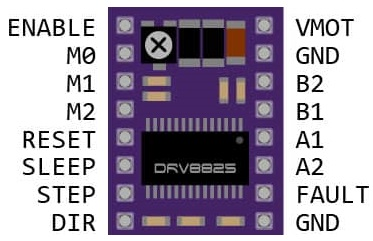
\includegraphics[height=4.5cm]{images/drv8825 pinmap.jpg}
        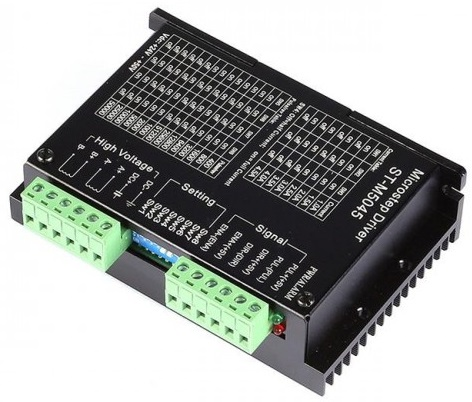
\includegraphics[height=4.5cm]{images/st-m5045.jpg}
    \end{center}
        \begin{tikzpicture} [remember picture, overlay]
        \node at (2.0, 0.5) {(a)};
        \node at (8.5, 0.5) {(b)}; %1.1
        \end{tikzpicture}	
        \caption{Motor drivers - (a) DRV8825 (b) ST-M5045}
        \label{Circuit - PCB, Schematic}
\end{figure}

\begin{table}[H]
    \centering
    \captionsetup{justification = centering}
    \begin{tabular}{ll}
        \hline
        % Number of full bridges           & 2                  \\
        Vs (min) $(\mathrm{V})$                     & 8.2                \\
        Vs ABS (max) $(\mathrm{V})$                 & 47                 \\
        Full-scale current $(\mathrm{A})$           & 2.5                \\
        Peak output current $(\mathrm{A})$          & 3                  \\
        RDS(ON) (HS + LS) $(\mathrm{m\Omega})$           & 400                \\
        Sleep current $(\mathrm{\mu A})$               & 10                 \\
        Control mode                     & STEP/DIR           \\
        Control interface                & Hardware (GPIO)    \\
        \textbf{Microstepping levels}             & \textbf{32}                 \\
        % Features                         & Current Regulation \\
        % Rating                           & Catalog            \\
        Operating temperature range $(\mathrm{\deg C})$ & -40 to 85         \\
        \hline
    \end{tabular}%
    \caption{Specification of \textit{DRV8825}}
    \label{Specification of DRV8825}
\end{table}

\begin{table}[H]
    \centering
    \captionsetup{justification=centering}
    \begin{tabular}{ll}
        \hline
        \textbf{DC power input type $(\mathrm{V})$}  & \textbf{24$\sim$50}      \\
        \textbf{Output current $(\mathrm{A})$}       & \textbf{1$\sim$4.5}      \\
        \textbf{Mircostep}           & \textbf{2, 4, 8, 16, 32, 64, 128, 256, 5, 10, 25, 50, 125, 250               }                \\
        Protect form        & Overheated, Short-voltage, over-voltage, over-current protection \\
        Maximum pulse rate $(\mathrm{kHz})$ & 300             \\
        Dimensions               & $120\mathrm{~mm}\times92\mathrm{~mm}\times33\mathrm{~mm}$ \\
        % Weight                   & \textless{}280g \\
        Working environment & Temperature-$15\sim40\mathrm{\deg C}$, Humidity\textless{}$90\%$ \\ 
        \hline
    \end{tabular}
    \caption{Specification of \textit{ST-M5045}}
    \label{Specification of ST-M5045}
\end{table}

Though DRV8825 is a small diode, it could function as well as other motor drivers, and it could be added to the PCB design so that the motor is controlled directly. But it tended to malfunction at high speeds and acceleration conditions. It's mainly due to the affordable voltage and current of the diode, and ST-M5045 was used for better control at higher voltage and current conditions. Also, the number of steps for each diode could be changed, which is related to the pulse is frequency. ST-M5045 is an exterior step motor driver and there are several switches at the side for changing the current and number of steps. To supply the whole system with proper power, a transformer is demanded. $24\mathrm{~V}$ SMPS converts AC voltage to DC $24\mathrm{V}$ and other versions can supply $36\mathrm{V}$ and $48\mathrm{V}$. With all these diodes, the final circuit was designed. (Figure \ref{Circuit - PCB, Schematic}).

\begin{figure}[H]
    \begin{center}
        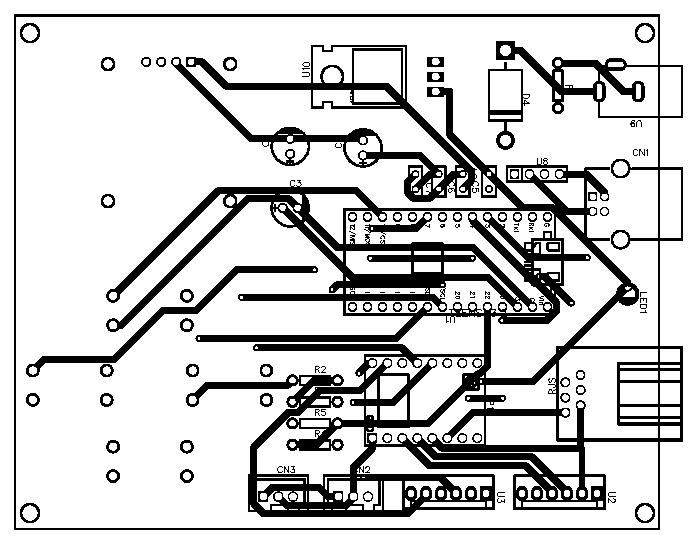
\includegraphics[width=9cm, angle=90]{images/Circuit(PCB).pdf}
        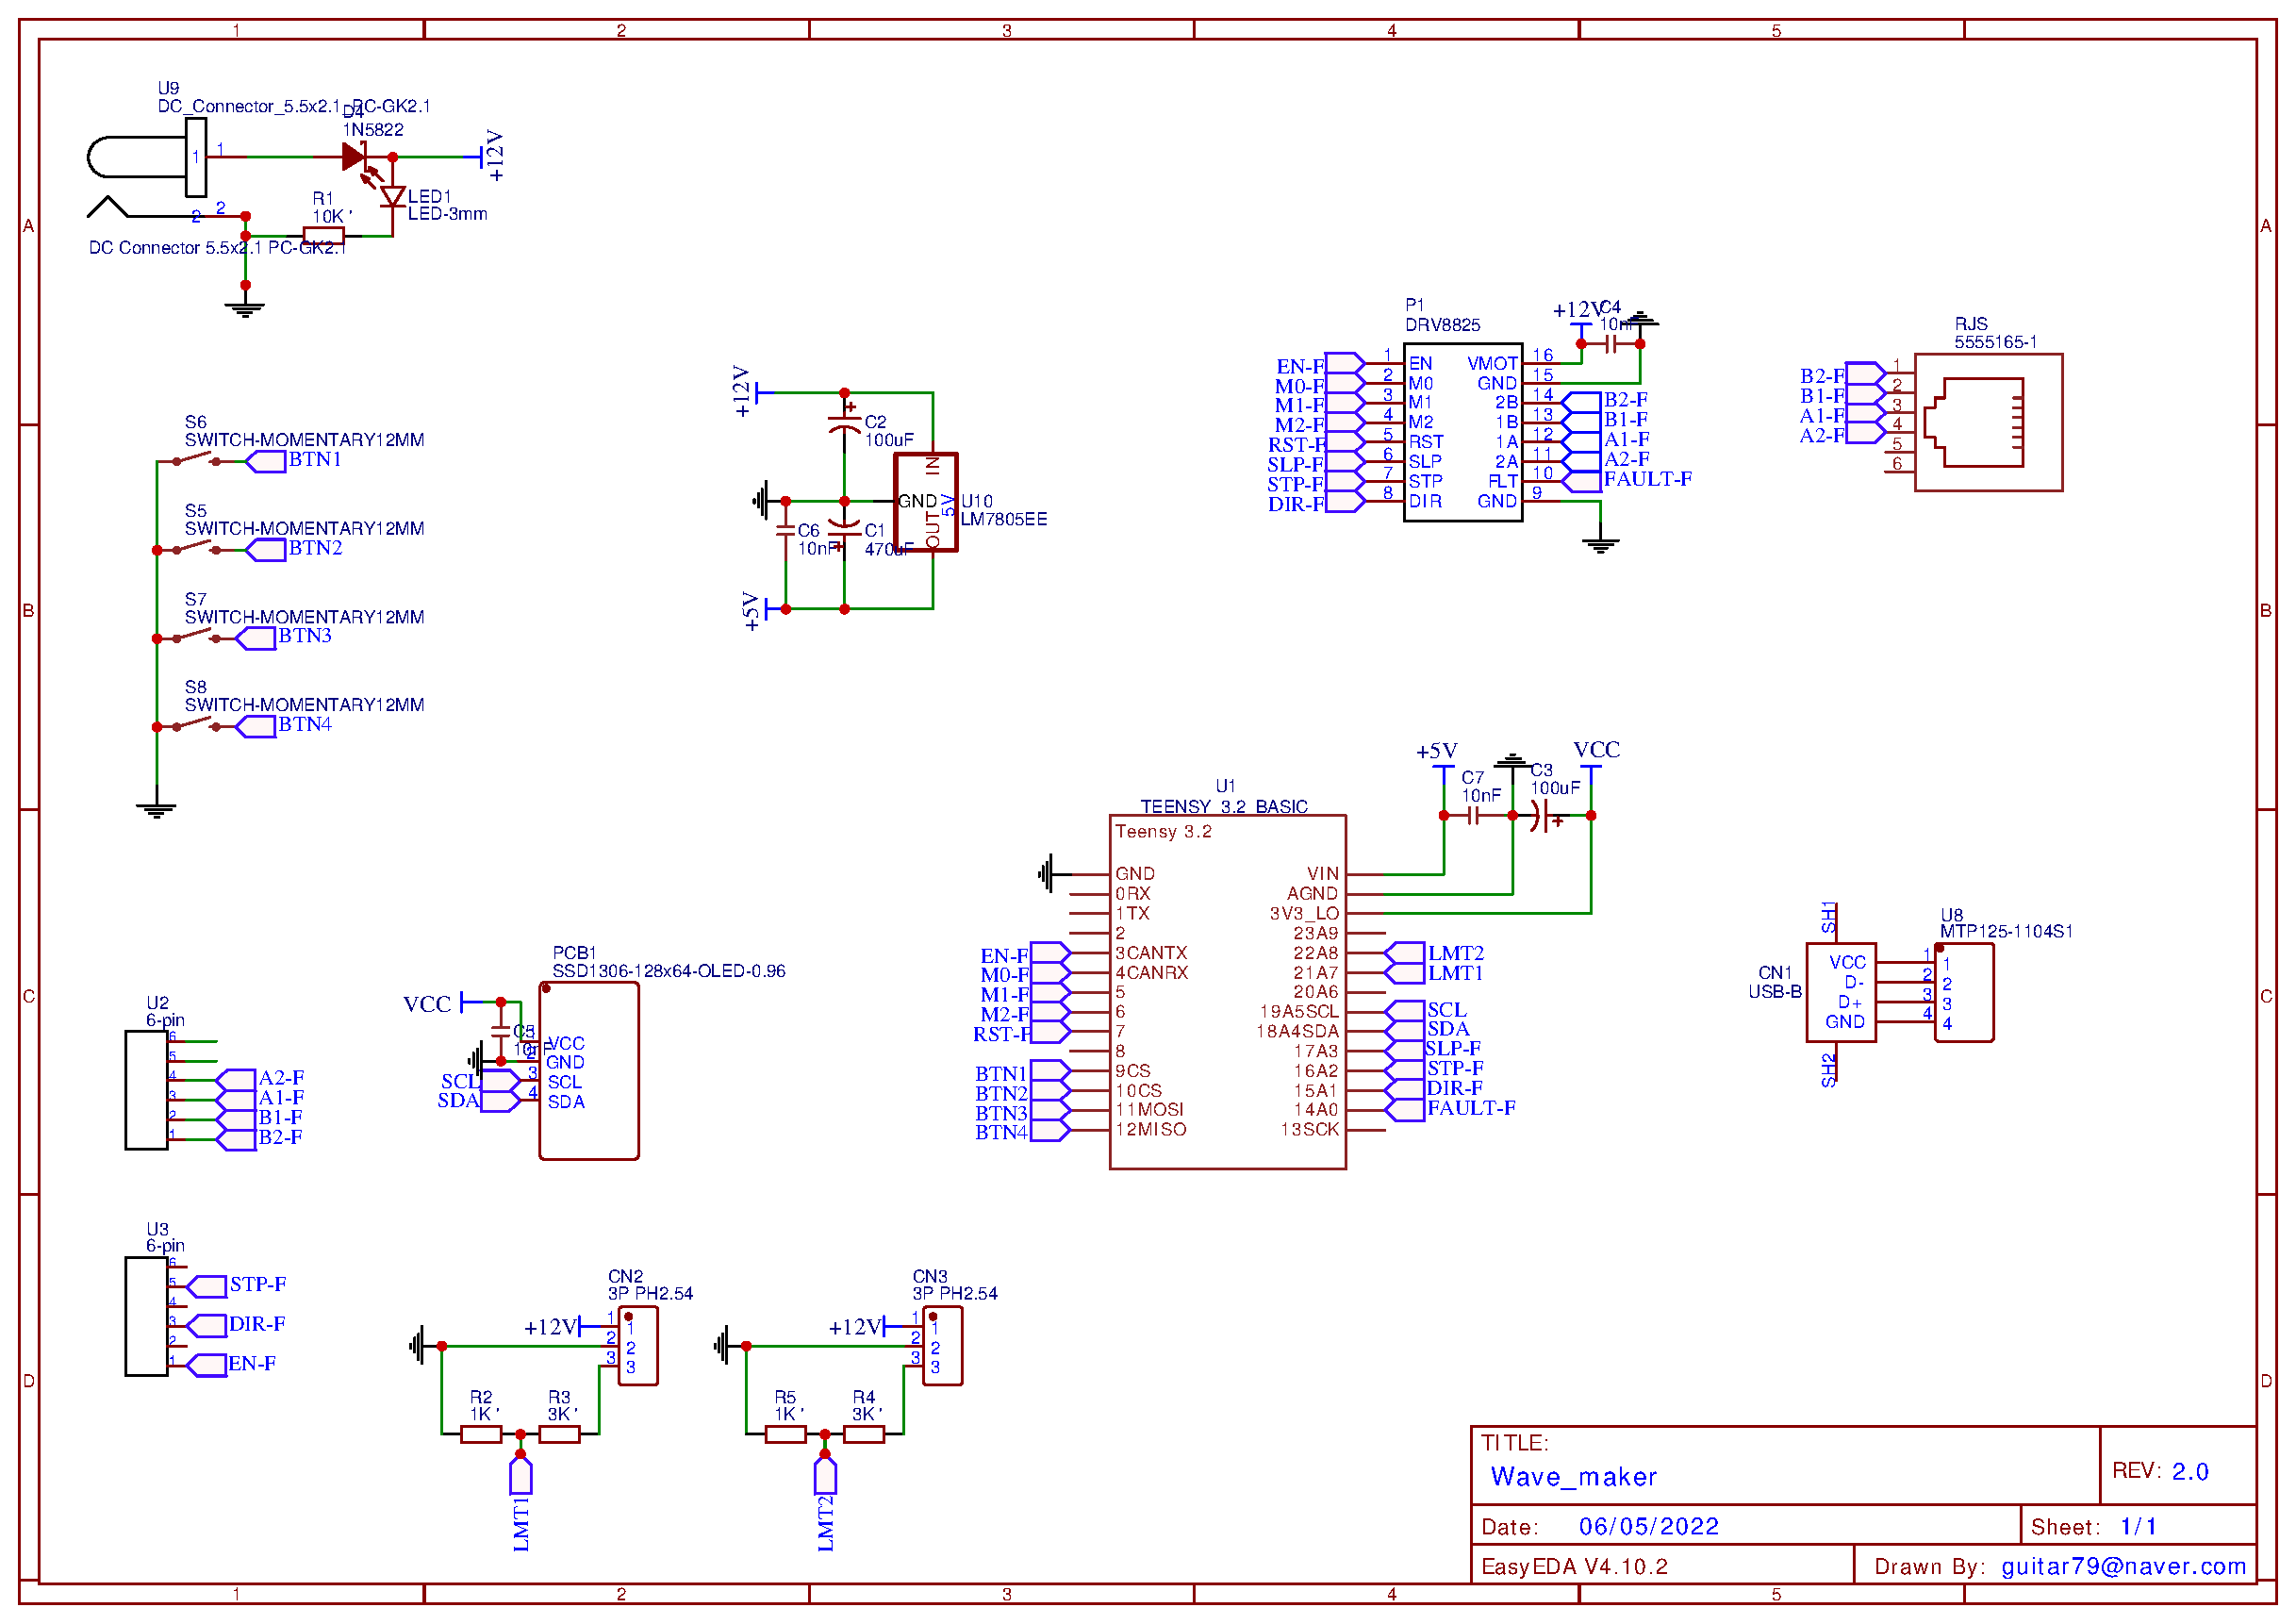
\includegraphics[width=9cm, angle=90]{images/Circuit(Schematic).pdf}
    \end{center}
        \begin{tikzpicture} [remember picture, overlay]
        \node at (0.9, 0.5) {(a)};
        \node at (7.9, 0.5) {(b)}; %1.1
        \end{tikzpicture}	
        \caption{Circuit - (a) PCB (b) Schematic diagram}
        \label{Circuit - PCB, Schematic}
\end{figure}

\subsubsection{Coding}
First of all, a fundamental code was made, which moves the plate back and forth. There are various libraries for driving a step motor and AccelStepper was used for it. Most of the libraries control the rotational speed of the motor. In the case of AccelStepper, it sets the angular velocity of the motor or the increment of the angular displacement, moving on a uniform velocity. 

\begin{algorithm}[H]
    \caption{Linear Movment}
    \label{Linear Movement}
    \begin{algorithmic}[1]
    \Statex Stepper motor(stepPin, dirPin);
    \Statex StepControl controller;
    \State \Comment{These variables and parameters should be defined priory}
    \Procedure{Linear Movement}{}\Comment{Move the motor back and forth}
        \Function {move motor}{$A$}
            \State motor.setTargetRel($A$);
            \State \Comment{moves the motor by $A$ steps}
            \State controller.move(motor);
            \State \Comment{$delay(time)$ is required!}
        \EndFunction
    \EndProcedure
    \end{algorithmic}
\end{algorithm}

The motor moved far slower than the expectation. Even though the maximum angular velocity and its angular displacement were set, the motor had limits according to the voltage, current, and performance of the motor driver. The transformer was changed so that higher voltage and current can flow through the circuit. It's raised to $36\mathrm{~V}$ from $24\mathrm{~V}$. Also, the code had changed. The new library is Teensystep \cite{luni64}. It can set the angular displacement of the motor as a function of time. By substituting the function from Algorithm \ref{Sinusoidal Motion}, a simple transverse motion and a sinusoidal move were able to be performed.

\begin{algorithm}[H]
    \caption{Time-based Motion}
    \label{Sinusoidal Motion}
    \begin{algorithmic}[1]
    \Procedure{Motion}{$A, \Delta t, \Delta\phi$}\Comment{Move the motor by setting angular displacement}
        \For{$elapsed Time \geq 0$}
            \If{$elapsed Time$ $\geq$ $\Delta t$}
                \State {$elapsed Time$ = 0}
                \State {$target = f(n)$}\Comment{For the sinusoidal motion, $target$ = $A \sin${($n$ $\Delta$$\phi$)}}
                % \State {$target$ = $A \sin${($n$ $\Delta$$\phi$)}}
                \State {$n$ $\gets$ $n$ + 1}
                \State {Move $motor$ to $target$}
            \EndIf
        \EndFor
        \EndProcedure
    \end{algorithmic}
\end{algorithm}

From Algorithm \ref{Sinusoidal Motion}, $f(n)$ is a function of dummy variable $n$, which sets $target$ - the angular displacement of the step motor - and $n$ is incremented by 1 in every $elapsedTime$. The code functions by setting the angular velocity of the motor based on $f(n)$, and there are other factors multiplied by it. $f(n) = A\sin{n \Delta\phi}$ is used to generate sinusoidal movement, with the proper value for the parameters. Here is an explanation of the parameters:
\begin{itemize}
    \item $A$

    It's the amplitude of the motion. Ideally, the plate should oscillate with the amplitude of $A$. It is measured in $step$, and it was known that 1$\mathrm{~cm}$ is equal to 400$\mathrm{~step}$, so the actual amplitude of the plate is $A/400$ in $\mathrm{~cm}$.

    \item $\Delta\phi$

    It's the increment of the phase of the displacement function with the dimension of $\mathrm{rad}$.

    \item $\Delta t$

    It's the value of $elapsedTime$ in the Algorithm \ref{Sinusoidal Motion}. Measured in $\mathrm{ms}$ with $millis()$, it sets the time interval for increasing dummy variable $n$.
\end{itemize}

The phase velocity(the rate at which phase of the function $f(n)$ changes) is derived as:
\begin{equation}
    \omega = \frac{\Delta\phi}{\Delta t}
    \label{Code: Omega}
\end{equation}

By setting $A$, $N(=\Delta t)$ and $\omega$ as a new parameter, $\Delta \phi$ is deleted and $f(n)$ as a function of $\omega$ is derived:
\begin{equation}
    f(n) = A\sin{N\omega}
    \label{Code: New f(n) with parameter omega}
\end{equation}

The whole process of the wavemaker is shown in Figure \ref{Flow chart of the wave generating system}. As the parameters were set, the plate was moved by the code, and the wave was generated.

\begin{figure}[H]
    \centering
    \captionsetup{justification=centering}
    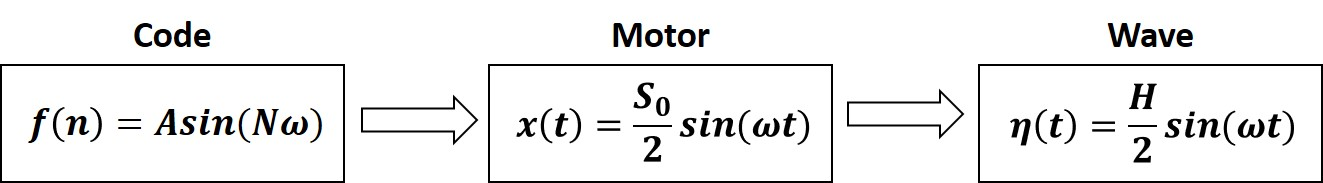
\includegraphics[width=12cm]{images/Flow_Chart(Analysis System).jpg}
    \caption{Flow chart of the wave generating system}
    \label{Flow chart of the wave generating system}
\end{figure}

All three sinusoidal functions share the same phase velocity $\omega$, and amplitudes have certain relations in between(Refer to Equation \ref{eq_023} and description of the parameters).

\subsection{Wave Gauge}%Check!

% \begin{figure}[H]
%     \begin{center}
%         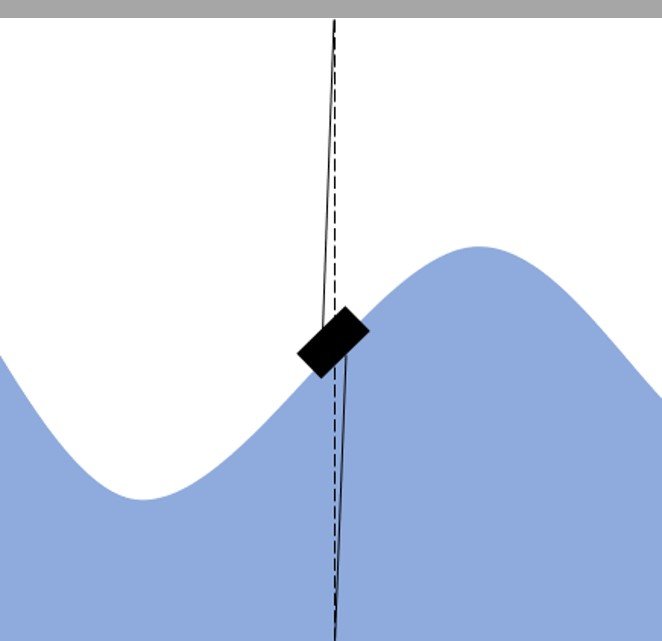
\includegraphics[height=6cm]{images/Wave_Gauge(Illustrated).jpg}
%         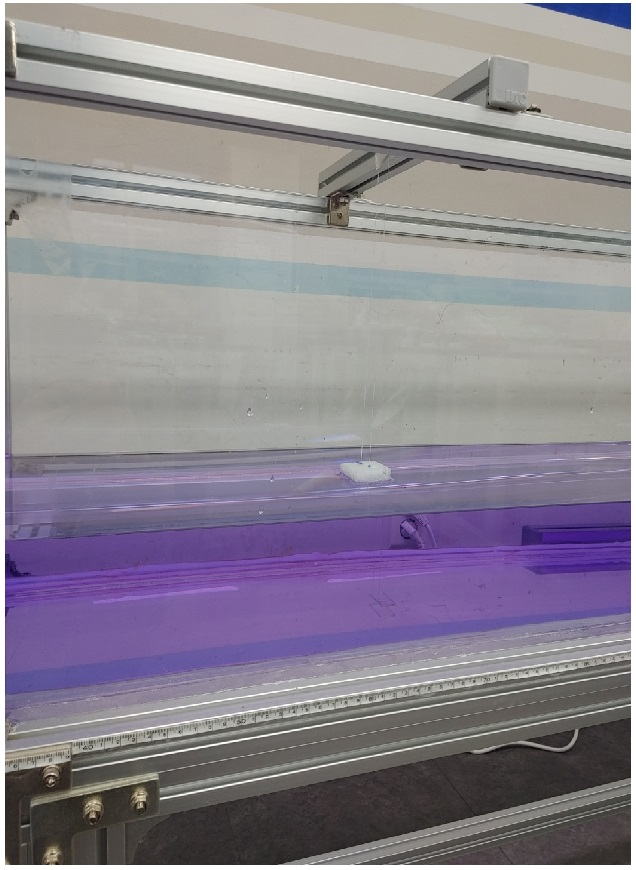
\includegraphics[height=6cm]{images/Wave_Gauge.jpg}
%     \end{center}
%         \begin{tikzpicture} [remember picture, overlay]
%         \node at (2.0, 0.5) {(a)};
%         \node at (7.0, 0.5) {(b)}; %1.1
%         \end{tikzpicture}	
%         \caption{Wave gauge - (a) Illustration (b) }
%         \label{Wave gauge}
% \end{figure}

\begin{figure}[H]
    \centering
    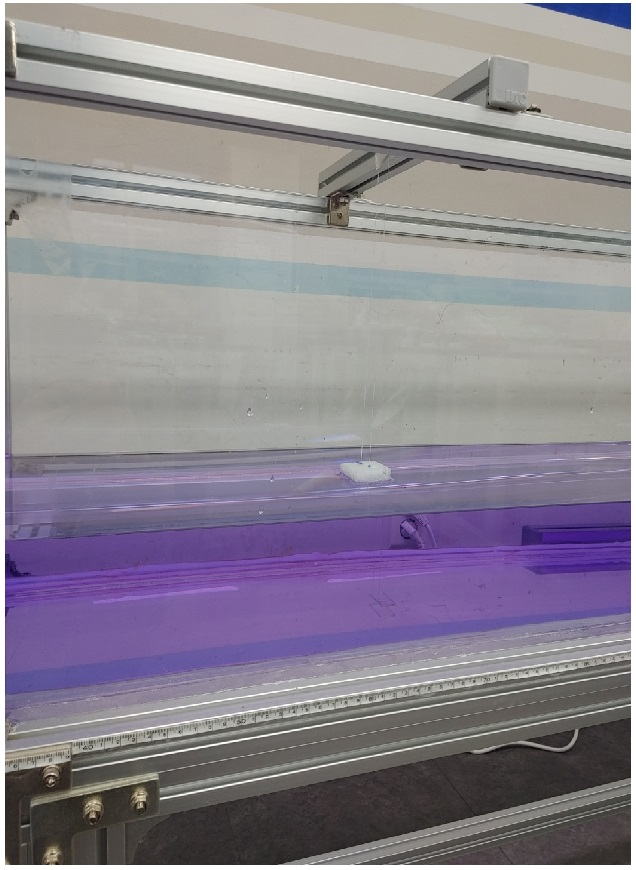
\includegraphics[height=8cm]{images/Wave_Gauge.jpg}
    \caption{Wave gauge}
    \label{Wave gauge}
\end{figure}

Wave height data was needed to derive the phase velocity and amplitude of the wave. A buoy was put on the water to measure the wave height and its movement was recorded. The buoy was fixed horizontally so that only the vertical movement was tracked properly. The size of the buoy was small so it don't affect the wave. A piece of Styrofoam was used, and it was fixed to the bottom and an assistant metal bar at the top of the wave channel with a thin string (Figure \ref{Wave gauge}). A dot was drew on one side of the buoy for video analysis, but it kept rotating by the external impulse. So, two strings were used to stop the rotation.
%Bookmark
Also, the water was pigmented blue to increase the contrast between the water and the buoy. It gives a better condition for the Tracker program, a video tracking \& analyzing tool.

\subsection{Code Test}
\begin{align*}
    Code: f(n) &= A \sin{N \omega_{1}}\\
    Motor: x(t) &= S_{0} \sin{\omega_{2} t}\\
    Wave: \eta(t) &= H \sin{\omega_{3} t}
\end{align*}

Out of the three sinusoidal waves shown above, the following is assumed:
\begin{align*}
    Amplitude&: A = S_0, H = \frac{4 S_0 \sinh^2 {kh}}{\sinh{2kh} + 2kh}\\
    Frequency&: \omega_{1} = \omega_{2} = \omega_{3}
\end{align*}

From testing out the code with the small motor and comparing $f(n)$ and $x(t)$, the phase velocity had agreed, but the amplitude was different (Figure \ref{PreExperiment}).

\begin{figure}[H]
    \centering
    \begin{tabular}{ll}
        \begin{filecontents*}{A.dat}
w_msr	A_thm	A_msr
0.6272	10	9.515
0.6275	10	9.532
0.6541	10	9.523
0.6681	10	9.499
0.6826	10	9.48
0.6978	10	9.456
0.6978	10	9.449
0.7849	10	9.326
0.785	10	9.318
0.8263	10	9.26
0.8971	10	9.138
0.8971	10	9.137
1.047	10	8.883
1.047	10	8.876
1.256	10	8.498
1.256	10	8.492
1.57	10	7.916
1.57	10	7.903
1.744	10	7.588
1.962	10	7.206
1.962	10	7.197
2.093	10	6.988
2.093	10	6.978
2.243	10	6.749
2.415	10	6.489
2.617	10	6.218
2.618   10	6.214
3.141	10	4.837
3.141	10	4.837
3.927	10	3.093
5.236	10	0.5795
        \end{filecontents*}

        \begin{tikzpicture}[
                %Environment Cfg.
                %font=\bfseries\sffamily,
            ]
            \begin{axis}[
                width=7cm,
                height=7cm,
                at={(0,0)},
                ymin=0,
                ymax=13,
                xmin=0,
                xmax=6,
                grid=both,
                minor tick num =5,
                minor tick style={draw=none},
                minor grid style={thin,color=black!10},
                major grid style={thin,color=black!10},
                %ylabel style={rotate=90},
                ylabel={$A_{plate}~\left[\mathrm{~cm}\right]$},
                xlabel={$\omega_{msr}~\left[\mathrm{~rad/s}\right]$},
                tick align=outside,
                axis x line*=middle,
                axis y line*=none,
                xtick={0,2,...,16},
                ytick={0,2,...,16},
                %xlabel style={color=blue!50!cyan},
                %ylabel style={align=center,rotate=-90,color=blue!50!cyan},
                x tick label style={
                    /pgf/number format/assume math mode, font=\sf\scriptsize},
                y tick label style={
                    /pgf/number format/assume math mode, font=\sf\scriptsize},
                legend cell align = {left},
                legend pos = north west,
                legend style={nodes={scale=0.5, transform shape}},
                ]
                \addplot [%only marks, 
                    mark size=1pt,
                    mark=o, 
                    %mark options={solid}, 
                    %smooth,
                    ] 
                table [x=w_msr, y=A_thm] {A.dat};
                \addlegendentry{$A_{thm} - \omega_{msr}$}
                \addplot [%only marks, 
                    mark = +,
                    mark size=1pt,
                    ]
                table [x=w_msr, y=A_msr] {A.dat};
                \addlegendentry{$A_{msr} - \omega_{msr}$}
            \end{axis}
        \end{tikzpicture}
        
        &
        
        \begin{filecontents}{B.dat}
                    wthm   wPlate
0.6283	0.6272
0.6981	0.6978
0.7854	0.785
0.8976	0.8971
1.0472	1.047
1.2566	1.256
1.5708	1.57
1.9635	1.962
2.0944	2.093
2.6180	2.617
3.1416	3.141
3.9270	3.918
5.2360	5.236
4.4880	4.487
3.9270	3.919
3.4907	3.49
0.6283	0.6275
0.6545	0.6541
0.6684	0.6681
0.6830	0.6826
0.6981	0.6978
0.7854	0.7849
0.8267	0.8263
0.8976	0.8971
1.0472	1.047
1.2566	1.256
1.5708	1.57
1.7453	1.744
1.9635	1.962
2.0944	2.093
2.2440	2.243
2.4166	2.415
2.6180	2.617
3.1416	3.141
            \end{filecontents}
        
            \begin{tikzpicture}[
                    %Environment Cfg.
                    font=\bfseries\sffamily,
                ]
                    \begin{axis}[
                        width=7cm,
                        height=7cm,
                        at={(0,0)},
                        ymin=0,
                        ymax=6,
                        xmin=0,
                        xmax=6,
                        grid=both,
                        minor tick num =5,
                        minor tick style={draw=none},
                        minor grid style={thin,color=black!10},
                        major grid style={thin,color=black!10},
                        %ylabel style={rotate=90},
                        ylabel={$\omega_{msr}~\left[\mathrm{rad/s}\right]$},
                        xlabel={$\omega_{thm}~\left[\mathrm{rad/s}\right]$},
                        tick align=outside,
                        axis x line*=middle,
                        axis y line*=none,
                        xtick={0,2,...,16},
                        ytick={0,2,...,16},
                        %xlabel style={color=blue!50!cyan},
                        %ylabel style={align=center,rotate=-90,color=blue!50!cyan},
                        x tick label style={
                            /pgf/number format/assume math mode, font=\sf\scriptsize},
                        y tick label style={
                        /pgf/number format/assume math mode, font=\sf\scriptsize},
                        legend cell align = {left},
                        legend pos = north west,
                        legend style={nodes={scale=0.5, transform shape}},
                        ]
                        \addplot [only marks, 
                            mark size=1pt,
                            mark=o, 
                            ]
                            table [x=wthm, y=wPlate] {B.dat};
                           \addlegendentry{$ \omega_{msr} - \omega_{thm}$}
                    \end{axis}
        \end{tikzpicture}
    \end{tabular}
    
    \begin{tikzpicture} [remember picture, overlay]
        \node at (-5.8, 0.6) {\scriptsize{(a)}};
        \node at (2.0, 0.6) {\scriptsize{(b)}};
    \end{tikzpicture}
    \caption{$\omega_{msr} - \omega_{thm}$ graph - (a) wave (b) plate}
    \label{PreExperiment}
\end{figure}

% \begin{figure}[H]
%     \centering
%     \captionsetup{justification=centering}
%     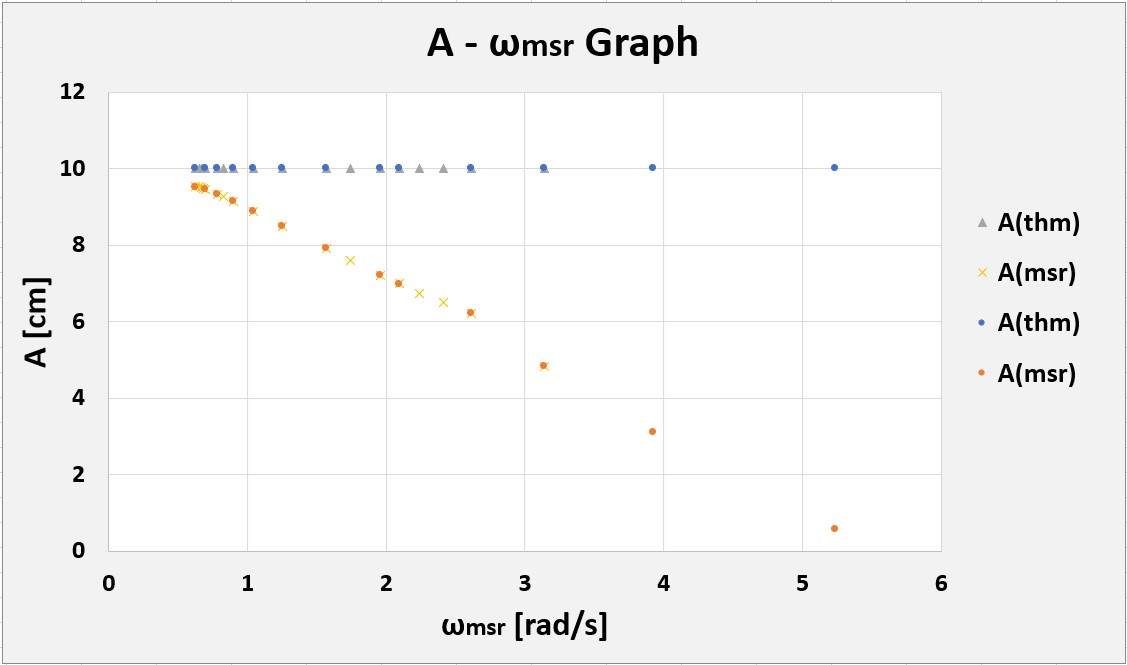
\includegraphics[width=12cm]{images/PreExperiment_Graph(A-Omega).jpg}
%     \caption{$A - \omega_{msr}$ Graph of motor}
%     \label{PreExperiment Graph(A - Omega)}
% \end{figure}

Angular displacement data had been collected from the Serial monitor and transitional data of the plate had been collected by tracking its movement from the video. $\omega$ was varied by changing $\Delta\phi$ and $N$. $A$ was fixed to $10\mathrm{cm}$ and it's expected to be consistent for the plate's motion. But instead, the measured amplitude had been smaller, and it seemed to decrease as $\omega$ increased. From Figure \ref{Circuit - PCB, Schematic}, orange dots were collected by changing $N$, and yellow dots were collected by changing $\Delta\phi$ (However, $\omega_{msr}$ refers to the measured value and $\omega_{thm}$ refers to the theoretically predicted value. $_{msr}$ and $_{thm}$ notation is used throughout the whole paper).

Unlike amplitude, $\omega_{msr}$ (measured $\omega$) agreed with $\omega_{thm}$ ($\omega$ in the code) with high precision. (Figure \ref{PreExperiment Graph(Omega - Omega)}). The best-fit line was $y=0.999510x$ with $R^2 = 1.000000$.

% \begin{figure}[H]
%     \centering
%     %\captionsetup{justification=centering}
%     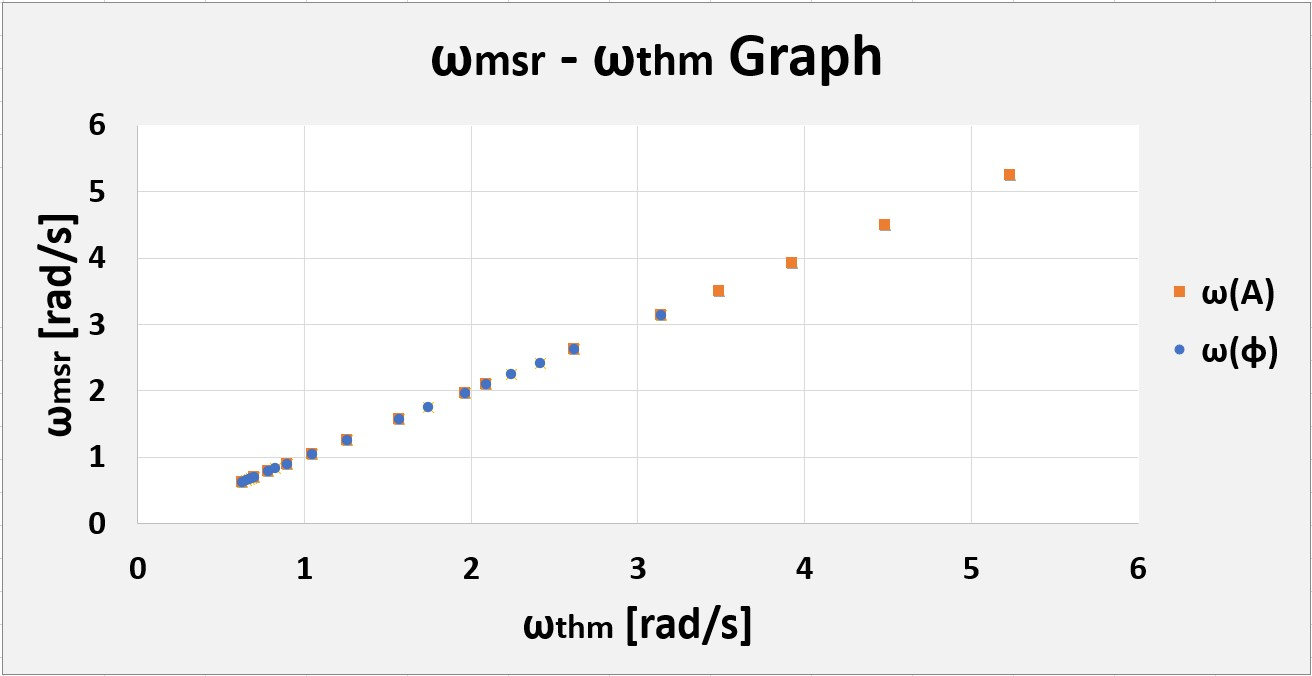
\includegraphics[width=12cm]{images/PreExperiment_Graph(Omega-Omega).jpg}
%     \caption{$\omega_{msr} - \omega_{thm}$ Graph of motor}
%     \label{PreExperiment Graph(Omega - Omega)}
% \end{figure}




It's concluded that this phenomenon was due to the limitation of the motor, related to parameters MaxSpeed and MaxAcceleration. The amplitude could be increased but the difference was inevitable. As $\omega$ increased, the plate couldn't catch up with the expected motion speed and acceleration. The reason is that the motor worked by calculating the velocity difference between the current and next states, and moved to the target though it hadn't reached the expected velocity. It resulted in a smaller amplitude and the wave got distorted. MaxSpeed and MaxAcceleration were set from the code but they're just numbers, and to increase the performance of the motor, provided voltage and current were raised. This problem was approached from a basic power supply issue.

Since $A$ and $S_{0}$ were different, three waves needed to be compared: signal from the code (angular displacement of the step motor), movement of the plate (transitional displacement), and progressive wave from in the channel(Figure \ref{Flow chart of the wave generating system}). There was no information of a relation between $A$ and $S_{0}$. The trend doesn't fit in $y=1/x$ (MaxSpeed = (const)) or $y=1/x^{2}$ (MaxAcceleration = (const)), and there were no other distinct trends related. But it's still assumed that the relation between $S_{0}$ and $H$ holds, and the relation between $A$ and $S_{0}$ will be collected for interpolation.

\subsection{Experimental Setup}
From the Code Test and Froude Similarity Law, various conditions for the experiments were set as $A~=~1,~2,~...,~10\mathrm{~cm}$ and $\omega~=~0.5\pi,~\pi,~...,~4.0\pi$. But, there had been some unexpected issues, and $\omega$ had changed to $3,~4,~6,~7,~9,~10,$ and $12\mathrm{~rad/s}$.


\begin{figure}[H]
    \begin{center}
        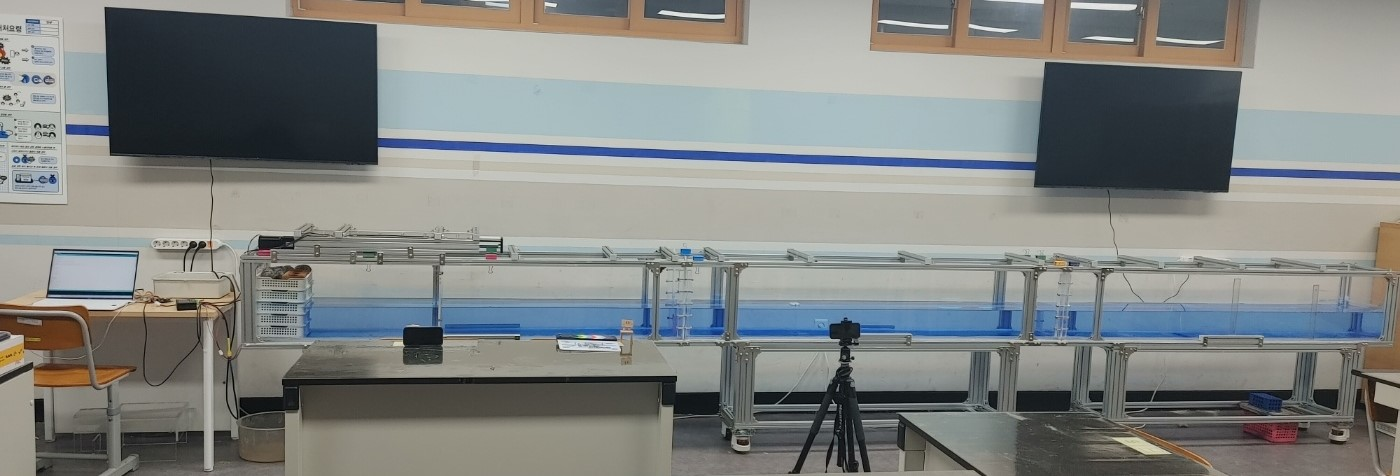
\includegraphics[width=\textwidth]{Experiment_System_Crop}
    \end{center}
        \begin{tikzpicture} [remember picture, overlay]
        \node [draw=yellow, text=yellow] (computer) at (1.0, 3.8) {\scriptsize{computer}};
        % \node [draw] (computer) at (1.0, 3.5) {.};
        % % arrows
        % \draw [->] (computer) -- (computerA) 
        \node [draw=yellow, text=yellow] at (4.6, 1.7) {\scriptsize{camera1}};
        \node [draw=yellow, text=yellow] at (9.5, 1.5) {\scriptsize{camera2}}; 
        \end{tikzpicture}	
        \caption{Experiment system - Laboratory}
        \label{Experimnet_System} 
\end{figure}


The system is shown in Figure \ref{Experimnet_System}. At the left end of the channel, the wave was generated, and there were two cameras beside the wave channel to collect data from the movement of the plate and the buoy. % 연구 과정
        \section{Result}

Assumptions were needed to be verified from the data: whether $\omega$ of all three waves agree, and the relation between $H$ and $S_{0}$ holds.

% \begin{figure}[H]
%     \centering
%     \includegraphics[width=0.48\textwidth]{images/Experiment(wthm-omega_msr)_Plate.jpg}
%     \includegraphics[width=0.48\textwidth]{images/Experiment(wthm-omega_msr)_Wave.jpg}
%     \caption{$\omega_{msr} - \omega_{thm}$ Graph of Plate(left) and Wave(right)}
%     \label{omega - omega graph1}
% \end{figure}

%https://tex.stackexchange.com/questions/11251/trend-line-or-line-of-best-fit-in-pgfplots
\begin{figure}[htbp]
    \centering
    \begin{tabular}{ll}
        \begin{filecontents*}{wthm-wwave.dat}
            wthm    wwave
            12  12.03
            12	11.91
            12	11.88
            12	11.96
            12	12.07
            12	12
            12	11.8
            12	12
            12	11.9
            12	11.77
            10	10.2
            10	10.1
            10	10.01
            10	10.07
            10	10.1
            10	10.07
            10	10.09
            10	10.05
            10	10.15
            10	9.84
            9	8.95
            9	9.02
            9	9
            9	9.02
            9	9.15
            9	9.28
            9	9.17
            9	8.94
            9	8.94
            9	8.94
            7	7.16
            7	6.99
            7	6.86
            7	6.99
            7	6.89
            7	6.85
            7	7.06
            7	6.89
            7	6.91
            7	6.9
            6	5.93
            6	5.96
            6	5.97
            6	5.94
            6	6.03
            6	5.73
            6	5.77
            6	5.76
            6	5.94
            6	5.79
            4	3.908
            4	3.984
            4	3.969
            4	3.982
            4	3.978
            4	4.082
            4	4.025
            4	4.051
            4	3.86
            4	3.784            
        \end{filecontents*}
    
        \begin{tikzpicture}[
                %Environment Cfg.
                %font=\bfseries\sffamily,
            ]
            \begin{axis}[
                width=7.5cm,
                height=7.5cm,
                at={(0,0)},
                ymin=0,
                ymax=15,
                xmin=0,
                xmax=15,
                grid=both,
                minor tick num =5,
                minor tick style={draw=none},
                minor grid style={thin,color=black!10},
                major grid style={thin,color=black!10},
                %ylabel style={rotate=90},
                ylabel={$\omega_{msr}~\left[\mathrm{rad}/s\right]$},
                xlabel={$\omega_{thm}~\left[\mathrm{rad}/s\right]$},
                tick align=outside,
                axis x line*=middle,
                axis y line*=none,
                xtick={0,2,...,16},
                ytick={0,2,...,16},
                %xlabel style={color=blue!50!cyan},
                %ylabel style={align=center,rotate=-90,color=blue!50!cyan},
                x tick label style={
                    /pgf/number format/assume math mode, font=\sf\scriptsize},
                y tick label style={
                    /pgf/number format/assume math mode, font=\sf\scriptsize},
                legend cell align = {left},
                legend pos = north west,
                legend style={nodes={scale=0.5, transform shape}},
                ]
                \addplot [only marks, 
                    mark size=1pt,
                    mark=o, 
                    %mark options={solid}, 
                    %smooth,
                    ] 
                    table [x=wthm, y=wwave] {wthm-wwave.dat};
                \addlegendentry{$ \omega_{msr}(wave) - \omega_{thm}$}
                \addplot [thick, red] table [y={create col/linear regression={y=wwave}}] {wthm-wwave.dat};
                \addlegendentry{
                    Linear regression: $ \omega_{msr} =
                    \pgfmathprintnumber{\pgfplotstableregressiona}
                    \cdot \omega_{thm}
                    \pgfmathprintnumber[print sign]{\pgfplotstableregressionb}$
                    };

                % \addplot[color=blue!50!cyan,smooth,tension=0.7,very thick] table [x index=0,y index=1,col sep=space] {Aplate-wmsrS.dat};
                % \addplot[color=cyan!50!lime,very thick] coordinates{(0,5)(25,5)};
                % \addplot[color=orange,very thick] coordinates{(0,11)(25,11)};
                % \addplot[color=red!80!orange,very thick] coordinates{(19,24.2)(23,24.2)};
                % \node[text=cyan!50!lime,fill=white,align=center,anchor=west,scale=0.8,inner sep=5pt] at (24.5,5){Base\\ Load};
                % \node[color=orange,fill=white,align=center,anchor=west,scale=0.8,inner sep=5pt] at (24.5,11){Average\\ Load};
                % \node[color=red!80!orange,fill=white,align=center,anchor=west,scale=0.8,inner sep=5pt] at (21.2,24.2){Maxium\\ Load};
            \end{axis}
        \end{tikzpicture}
        
        &
        
        \begin{filecontents}{wthm-wplate.dat}
                    wthm   wPlate
                    12	12.00
                    12	12.04
                    12	12.06
                    12	12.01
                    12	11.81
                    12	12.06
                    12	11.88
                    12	11.98
                    12	11.89
                    12	11.95
                    10	10.00
                    10	10.06
                    10	10.04
                    10	10.05
                    10	9.99
                    10	10.14
                    10	9.99
                    10	10.00
                    10	10.10
                    10	9.99
                    9	9.00
                    9	9.00
                    9	8.98
                    9	8.99
                    9	8.93
                    9	8.95
                    9	8.91
                    9	9.00
                    9	8.99
                    9	9.00
                    7	7.00
                    7	7.00
                    7	7.00
                    7	7.00
                    7	7.00
                    7	6.99
                    7	7.00
                    7	6.99
                    7	7.00
                    7	6.98
                    6	6.00
                    6	6.00
                    6	5.99
                    6	6.01
                    6	5.94
                    6	5.99
                    6	6.00
                    6	6.00
                    6	6.04
                    6	6.05
                    4	4
                    4	4
                    4	4.001
                    4	4.001
                    4	4.001
                    4	4.001
                    4	4
                    4	4
                    4	4.001
                    4	4.001   
            \end{filecontents}
        
            \begin{tikzpicture}[
                    %Environment Cfg.
                    font=\bfseries\sffamily,
                ]
                    \begin{axis}[
                        width=7.5cm,
                        height=7.5cm,
                        at={(0,0)},
                        ymin=0,
                        ymax=15,
                        xmin=0,
                        xmax=15,
                        grid=both,
                        minor tick num =5,
                        minor tick style={draw=none},
                        minor grid style={thin,color=black!10},
                        major grid style={thin,color=black!10},
                        %ylabel style={rotate=90},
                        ylabel={$\omega_{msr}~\left[\mathrm{rad}/s\right]$},
                        xlabel={$\omega_{thm}~\left[\mathrm{rad}/s\right]$},
                        tick align=outside,
                        axis x line*=middle,
                        axis y line*=none,
                        xtick={0,2,...,16},
                        ytick={0,2,...,16},
                        %xlabel style={color=blue!50!cyan},
                        %ylabel style={align=center,rotate=-90,color=blue!50!cyan},
                        x tick label style={
                            /pgf/number format/assume math mode, font=\sf\scriptsize},
                        y tick label style={
                        /pgf/number format/assume math mode, font=\sf\scriptsize},
                        legend cell align = {left},
                        legend pos = north west,
                        legend style={nodes={scale=0.5, transform shape}},
                        ]
                        \addplot [only marks, 
                            mark size=1pt,
                            mark=o, 
                            ]
                            table [x=wthm, y=wPlate] {wthm-wplate.dat};
                        \addplot [thick, red] table [y={create col/linear regression={y=wPlate}}] {wthm-wplate.dat};
                        \addlegendentry{$ \omega_{msr}(plate) - \omega_{thm}$}
                        \addlegendentry{
                            Linear regression: $ \omega_{msr} =
                            \pgfmathprintnumber{\pgfplotstableregressiona}
                            \cdot \omega_{thm}
                            \pgfmathprintnumber[print sign]{\pgfplotstableregressionb}$
                        };

                        % \addplot[color=blue!50!cyan,smooth,tension=0.7,very thick] table [x index=0,y index=1,col sep=space] {Aplate-wmsrS.dat};
                        % \addplot[color=cyan!50!lime,very thick] coordinates{(0,5)(25,5)};
                        % \addplot[color=orange,very thick] coordinates{(0,11)(25,11)};
                        % \addplot[color=red!80!orange,very thick] coordinates{(19,24.2)(23,24.2)};
                        % \node[text=cyan!50!lime,fill=white,align=center,anchor=west,scale=0.8,inner sep=5pt] at (24.5,5){Base\\ Load};
                        % \node[color=orange,fill=white,align=center,anchor=west,scale=0.8,inner sep=5pt] at (24.5,11){Average\\ Load};
                        % \node[color=red!80!orange,fill=white,align=center,anchor=west,scale=0.8,inner sep=5pt] at (21.2,24.2){Maxium\\ Load};
                    \end{axis}

        \end{tikzpicture}

    \end{tabular}
    
    \begin{tikzpicture} [remember picture, overlay]
        \node at (-5.8, 0.6) {\scriptsize{(a)}};
        \node at (2.0, 0.6) {\scriptsize{(b)}};
    \end{tikzpicture}
    \caption{$\omega_{msr} - \omega_{thm}$ graph - (a) wave (b) plate}
    \label{Experiment: omega - omega graph}
\end{figure}

Just as the assumption, $\omega$ was shared by the three waves. Both graphs of Figure \ref{Experiment: omega - omega graph} had a best-fit line with a high correlation coefficient $(R^2>0.99)$ and a slope close to 1.000. The statement 'slope = 1.0000' could be refuted by using a statistical test with $\sigma_{m}$ of the slope, but the uncertainty of the graph is relatively negligible due to the shape of the wave. It could be observed from the graphs such as Figure \ref{Data_omega=3_plate} (c). Though the wave height oscillates, it's not a clear sinusoidal wave and FFT was used to derive the dominant oscillation frequency and its amplitude. Most of the waves needed FFT analysis. The specific waveform of both waves in the channel and plate movement is provided in Appendix B, C. Also, the wave height data had intrinsic errors occurring from video tracking (Figure \ref{Tracker}).

\begin{figure}[H]
    \centering
    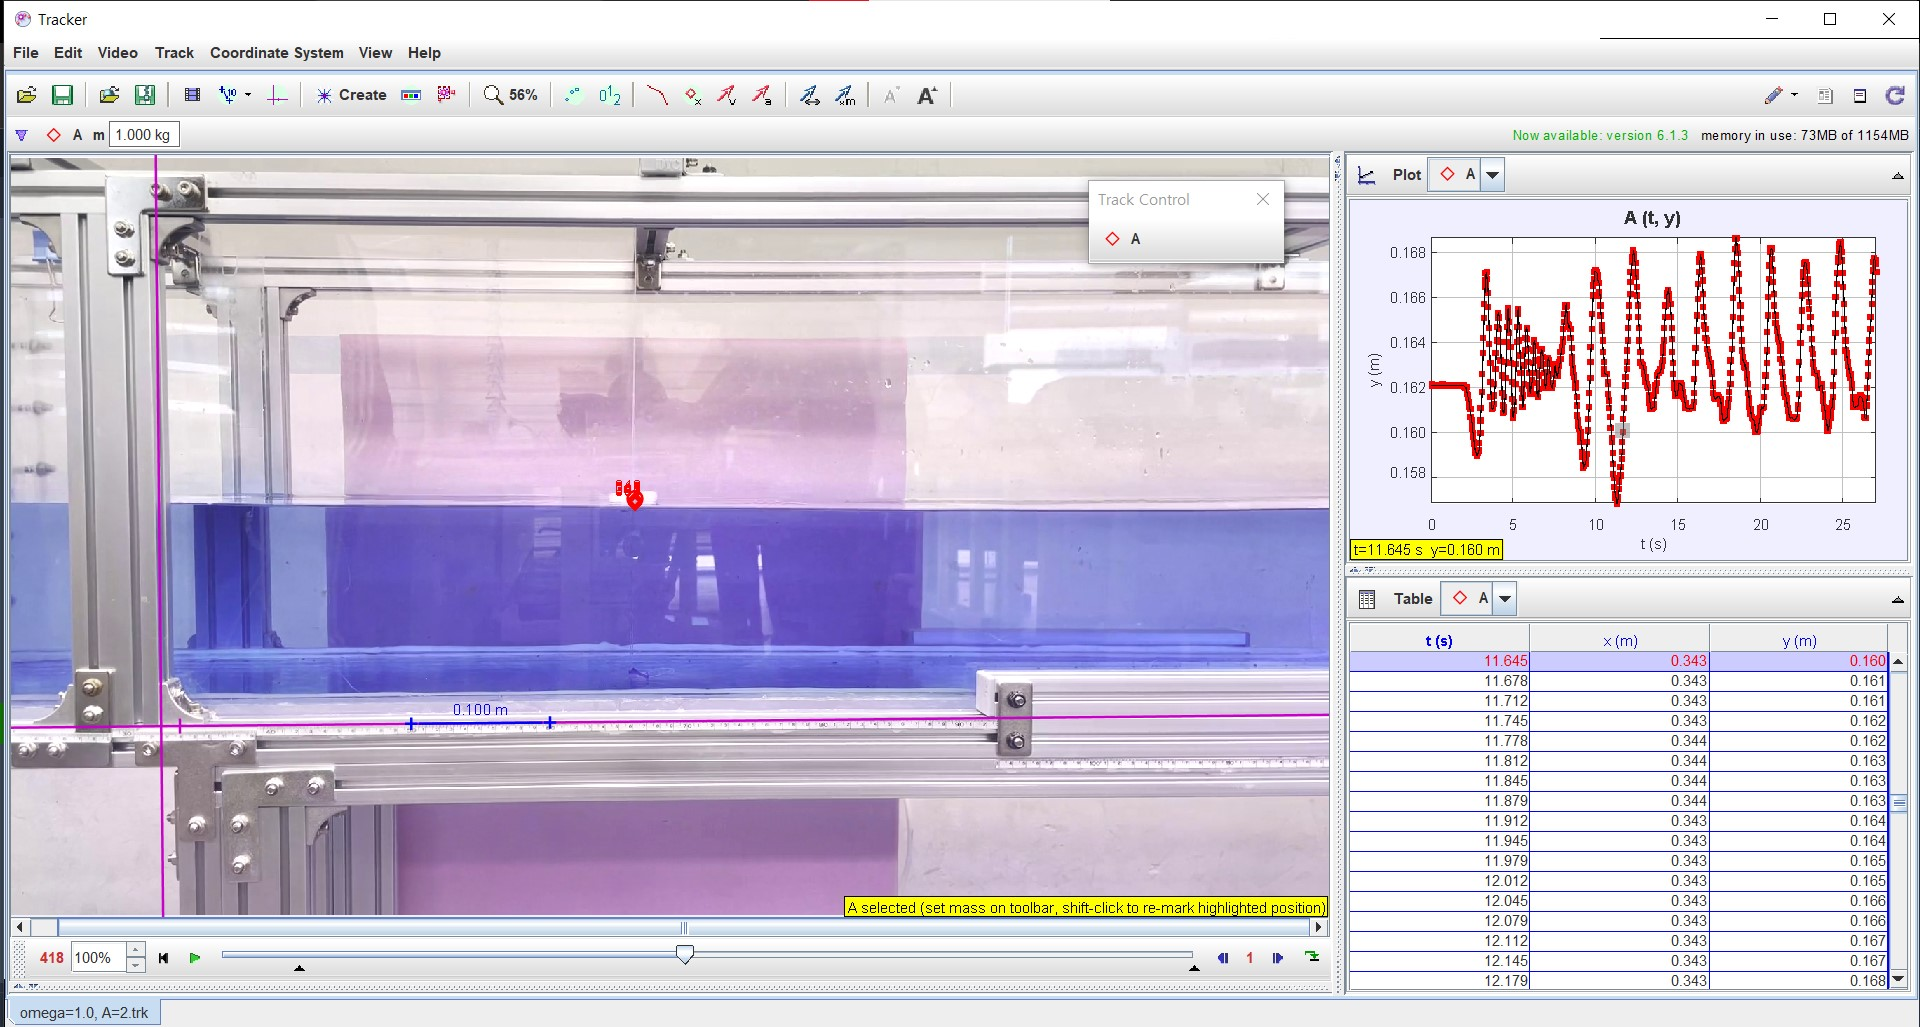
\includegraphics[width=\textwidth]{images/Experiment(Wave_Tracker, omega=1.0, A=2).jpg}
    \caption{Video Analysis}
    \label{Tracker}
\end{figure}

A black dot at one side of the buoy was tracked, but the piece of the styrofoam rotated as the wave progressed. Furthermore, the buoy submerged right under the surface on some occasions. Pointing out the surface was difficult for the cases. Testing out the data based on uncertainty is meaningless, and the statement 'slope = 1.0000' was said to be held for $\omega_{thm}$ and $\omega_{msr}$ for both plate and wave. Also, the plate moved too slowly with $\omega=3~(\sim \pi)$ that a wave was barely generated (Figure \ref{Data_omega=3_plate} (c)). The fluctuations at the front of the graph occurred from aligning the plate to the middle, and oscillation was tracked afterward: the amplitude($\sim \mathrm{cm}$) is negligible compared to the noise of the motor's rotation and its small movements.

Also, the phenomenon that $A$ decreasing as $\omega$ increasing had been observed:

\begin{figure}[H]
    \centering
        \begin{filecontents}{Aplate-wmsrS.dat}
                    wthm   A_plate
                    12	0.64
                    12	0.64
                    12	0.73
                    12	0.7
                    12	0.69
                    12	0.73
                    12	0.71
                    12	0.71
                    12	0.71
                    12	0.73
                    10	0.85
                    10	0.92
                    10	0.92
                    10	0.9
                    10	0.91
                    10	0.82
                    10	0.94
                    10	0.97
                    10	1.03
                    10	0.95
                    9	0.91
                    9	1.1
                    9	1.07
                    9	1.06
                    9	1.18
                    9	1.02
                    9	1.29
                    9	1.35
                    9	1.08
                    9	1.17
                    7	0.96
                    7	1.78
                    7	1.87
                    7	1.9
                    7	1.78
                    7	1.84
                    7	1.8
                    7	1.78
                    7	1.73
                    7	1.87
                    6	0.96
                    6	2.54
                    6	2.61
                    6	2.59
                    6	2.52
                    6	2.37
                    6	2.39
                    6	2.65
                    6	2.3
                    6	2.56
                    4	0.9566
                    4	1.913
                    4	2.856
                    4	3.795
                    4	4.744
                    4	5.313
                    4	5.568
                    4	5.662
                    4	5.677
                    4	5.681         
            \end{filecontents}
        
            \begin{tikzpicture}[
                    %Environment Cfg.
                    font=\bfseries\sffamily,
                ]
                    \begin{axis}[
                        width=0.75\textwidth,
                        height=8cm,
                        at={(0,0)},
                        ymin=0,
                        ymax=6,
                        xmin=0,
                        xmax=15,
                        grid=both,
                        minor tick num =5,
                        minor tick style={draw=none},
                        minor grid style={thin,color=black!10},
                        major grid style={thin,color=black!10},
                        %ylabel style={rotate=90},
                        ylabel={$A_{plate}~\left[\mathrm{cm}\right]$},
                        xlabel={$\omega_{msr}~\left[\mathrm{rad}/s\right]$},
                        tick align=outside,
                        axis x line*=middle,
                        axis y line*=none,
                        xtick={0,2,...,16},
                        ytick={0,1,...,6},
                        %xlabel style={color=blue!50!cyan},
                        %ylabel style={align=center,rotate=-90,color=blue!50!cyan},
                        x tick label style={
                            /pgf/number format/assume math mode, font=\sf\scriptsize},
                        y tick label style={
                        /pgf/number format/assume math mode, font=\sf\scriptsize},
                        ]
                        %\addplot[scatter, only marks] table [x index=0,y index=1,col sep=space] {Aplate-wmsrS.dat};
                        \addplot[scatter, 
                                only marks,
                                mark=o,
                                mark size=1pt,
                            ] 
                            table [x=wthm, y=A_plate] {Aplate-wmsrS.dat};
                        % \addplot[color=blue!50!cyan,smooth,tension=0.7,very thick] table [x index=0,y index=1,col sep=space] {Aplate-wmsrS.dat};
                        % \addplot[color=cyan!50!lime,very thick] coordinates{(0,5)(25,5)};
                        % \addplot[color=orange,very thick] coordinates{(0,11)(25,11)};
                        % \addplot[color=red!80!orange,very thick] coordinates{(19,24.2)(23,24.2)};
                        % \node[text=cyan!50!lime,fill=white,align=center,anchor=west,scale=0.8,inner sep=5pt] at (24.5,5){Base\\ Load};
                        % \node[color=orange,fill=white,align=center,anchor=west,scale=0.8,inner sep=5pt] at (24.5,11){Average\\ Load};
                        % \node[color=red!80!orange,fill=white,align=center,anchor=west,scale=0.8,inner sep=5pt] at (21.2,24.2){Maxium\\ Load};
                    \end{axis}
    
        \end{tikzpicture}
    \caption{$A_{plate} - \omega_{msr}$ graph}
    \label{A-omega graph}
\end{figure}

It's clear that $A_{plate}$ and $\omega_{msr}$ were negatively correlated, but the specific relation between them was not explicit: only the limiting value of $A_{plate}$ was known(since $A_{plate}$ converged as $A_{thm}$ increased).

As $\omega$ was set, it corresponds to unique $z(=kh)$ from dispersion relation:
\begin{equation}
    \omega^{2} = gk \tanh{kh} = \frac{g}{h} z ~\tanh{z}
    \label{dispersion_relation}
\end{equation}

The $z$ from Equation \ref{dispersion_relation} is the same value as the one in Equation \ref{eq_023}, and $H/S_{thm}$ could be derived. It was compared with $H/S_{msr}$, which could be calculated from the data set (Figure \ref{H/S graph}).

% \begin{figure}[H]
%     \centering
%     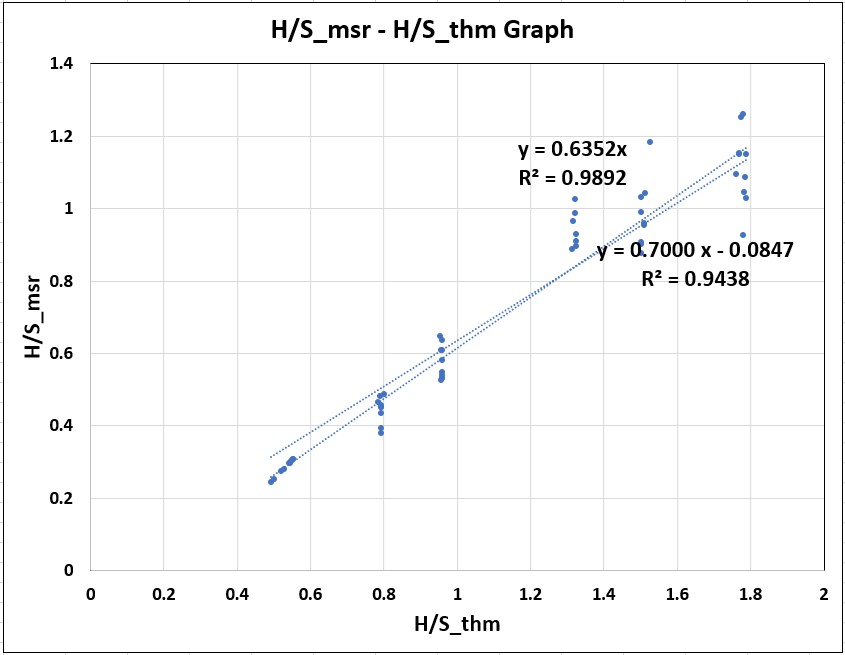
\includegraphics[width=\textwidth]{images/Experiment(H.S_thm-H.S_msr)_Proccessed_Data.jpg}https://www.overleaf.com/project/63aff5462256d537ece5848a
%     \caption{Caption}
%     \label{fig:enter-label1}
% \end{figure}

%https://tex.stackexchange.com/questions/11251/trend-line-or-line-of-best-fit-in-pgfplots
\begin{figure}[htbp]
    \centering
        \begin{filecontents}{HSthm-HSmsr.dat}
                HS_thm	HS_msr
                1.781440728	0.925436527
                1.785651376	1.085170025
                1.787735635	1.027713311
                1.782498659	1.045913291
                1.760671425	1.094309648
                1.787735635	1.15104453
                1.768471166	1.150212766
                1.77931432	1.26011236
                1.769571325	1.151819856
                1.776098332	1.252500343
                1.502818971	0.907053163
                1.512879552	1.042827713
                1.509535179	0.952282833
                1.51120852	0.957989748
                1.501134272	0.989520132
                1.526163172	1.182451424
                1.501302842	1.031007752
                1.502482211	0.900403351
                1.519540335	0.724198251
                1.501134272	0.877353529
                1.324569679	0.909190732
                1.324937643	0.929155313
                1.321072373	0.986915888
                1.323465588	1.024621212
                1.313331279	0.887096774
                1.315913161	0.964838394
                1.309086454	0.733436773
                1.326041332	0.895167286
                0.958556795	0.531089978
                0.958906454	0.580898876
                0.959081306	0.608042895
                0.958731617	0.530870712
                0.959081306	0.635545557
                0.956634768	0.607395324
                0.959431056	0.540311804
                0.95646013	0.524718468
                0.958556795	0.547893826
                0.954714602	0.645610278
                0.792888221	0.451327434
                0.792888221	0.377926685
                0.790392394	0.481381958
                0.793981875	0.44980695
                0.783557379	0.464839094
                0.791639619	0.434911243
                0.792419834	0.455155071
                0.79195164	0.393355983
                0.798366989	0.608601216
                0.800094292	0.48515625
                0.492276411	0.242943759
                0.528893957	0.280658651
                0.543862815	0.296883754
                0.553908234	0.308036891
                0.552905492	0.306913997
                0.542089448	0.294936947
                0.546948794	0.300287356
                0.551047756	0.304839279
                0.521368486	0.272679232
                0.499818992	0.25048407                  
            \end{filecontents}
        
            \begin{tikzpicture}[
                    %Environment Cfg.
                    font=\bfseries\sffamily,
                ]
                    \begin{axis}[
                        width=\textwidth,
                        height=10cm,
                        at={(0,0)},
                        ymin=0,
                        ymax=1.4,
                        xmin=0,
                        xmax=2,
                        grid=both,
                        minor tick num =5,
                        minor tick style={draw=none},
                        minor grid style={thin,color=black!10},
                        major grid style={thin,color=black!10},
                        %ylabel style={rotate=90},
                        ylabel={$H/S_{msr}$},
                        xlabel={$H/S_{thm}$},
                        tick align=outside,
                        axis x line*=middle,
                        axis y line*=none,
                        xtick={0,0.2,...,2},
                        ytick={0,0.2,...,2},
                        %xlabel style={color=blue!50!cyan},
                        %ylabel style={align=center,rotate=-90,color=blue!50!cyan},
                       x tick label style={
                            /pgf/number format/assume math mode, font=\sf\scriptsize},
                        y tick label style={
                            /pgf/number format/assume math mode, font=\sf\scriptsize},
                        legend cell align = {left},
                        legend pos = north west,
                        legend style={nodes={scale=0.5, transform shape}},
                        ]
                        \addplot[scatter, 
                                only marks, 
                                mark=o,
                                mark size=1.5pt,
                                color=black,
                            ] 
                        table [x=HS_thm, y=HS_msr] {HSthm-HSmsr.dat};    
                        \addplot [thick, red] table [y={create col/linear regression={y=HS_msr}}] {HSthm-HSmsr.dat};
                        %\addlegendentry{$y(x)$}
                        \addlegendentry{
                            Linear regression: $ \omega_{msr} =
                            \pgfmathprintnumber{\pgfplotstableregressiona}
                            \cdot \omega_{thm}
                            \pgfmathprintnumber[print sign]{\pgfplotstableregressionb}$
                        };

                        % \addplot[color=blue!50!cyan,smooth,tension=0.7,very thick] table [x index=0,y index=1,col sep=space] {Aplate-wmsrS.dat};
                        % \addplot[color=cyan!50!lime,very thick] coordinates{(0,5)(25,5)};
                        % \addplot[color=orange,very thick] coordinates{(0,11)(25,11)};
                        % \addplot[color=red!80!orange,very thick] coordinates{(19,24.2)(23,24.2)};
                        % \node[text=cyan!50!lime,fill=white,align=center,anchor=west,scale=0.8,inner sep=5pt] at (24.5,5){Base\\ Load};
                        % \node[color=orange,fill=white,align=center,anchor=west,scale=0.8,inner sep=5pt] at (24.5,11){Average\\ Load};
                        % \node[color=red!80!orange,fill=white,align=center,anchor=west,scale=0.8,inner sep=5pt] at (21.2,24.2){Maxium\\ Load};
                    \end{axis}
        \end{tikzpicture}
    \caption{$H/S_{msr} - H/S_{thm}$ graph}
    \label{H/S graph}
\end{figure}

 % 연구 결과
        %\section{Test Section}

Title : 21pt, bold face.

\subsection{Test Subsection}

Title : 16pt, bold face.

\subsubsection{Test Subsubsection}

Title : 14pt, normal style.

앞서 언급하였듯이 subsubsection, paragraph 와 같은 하위 절은 사용을 자제하는 것이 좋다.

\paragraph{Test Paragraph}

Title : 12pt, italic style. No numbering.

먼저 문장 속에서 수식을 사용하는 경우에는 \$ (수식) \$과 같이 처리하면 된다. 다음과 같이 작성한 후 컴파일을 하면
\begin{quote}
운동 에너지는 \$(1/2)mv$\wedge$2\$으로 표현된다. 여기서 \$m\$은 물체의 질량, \$v\$ 는 물체의 속력이다.
\end{quote}
pdf 파일에는 다음과 같이 나타난다.
\begin{quote}
운동 에너지는 $(1/2)mv^2$으로 표현된다. 여기서 $m$은 물체의 질량, $v$는 물체의 속력이다.
\end{quote}
위의 예시에서 보듯이 문장 속에서 수식을 사용할 때는 한 줄로 입력한다. 즉 분수 형태의 수식은 슬래쉬`/'로 대체하여 표현한다. 줄 간격을 일정하게 유지하기 위함이다.

다음은 수식이 문장 밖으로 나와 한 줄을 통째로 차지하는 경우이다. 수식을 작성하는 명령어는 다양하지만, 여기서는 equation, align에 대해서만 다룬다. 먼저 equation의 사용법을 예를 통해 확인해보자. 만약 다음과 같이 입력을 하고
\begin{lstlisting}
	\begin{equation}
	\int_V \nabla\cdot{\rm\bf F} dV = \oint_S {\rm\bf F}\cdot d{\rm\bf A}. \label{eq001}
	\end{equation}
\end{lstlisting}
컴파일을 하면 다음과 같은 식이 pdf파일에 나타나는 것을 확인할 수 있다.
\begin{equation}
\int_V \nabla\cdot{\rm\bf F} dV = \oint_S {\rm\bf F}\cdot d{\rm\bf A}. \label{eq001}
\end{equation}
문장 속에서 수식의 번호(라벨)을 호출하는 경우가 종종 있다. 이 때는 {\textbackslash}ref\{eq001\}을 사용하면 된다. 여기서 eq001은 수식에서 label 명령어 다음에 작성된 문구이다. 수식마다 각기 다른 라벨을 작성해야 하며 논문 저자가 기억하기 편한 것을 사용하면 된다. 서로 다른 수식에 중복된 라벨을 사용하면, 나중에 작성된 라벨의 수식 번호만 호출됨에 유의하라. 사용 예는 다음과 같다.
\begin{quote}
(작성 예) Divergence 이론은 임의의 벡터 필드 \${\textbackslash}rm{\textbackslash}bf F\$가 임의의 폐곡면 외부를 향하는 플럭스의 총량은 \${\textbackslash}nabla{\textbackslash}cdot\{{\textbackslash}rm{\textbackslash}bf F\}\$ 를 폐곡면 내부 부피에 대하여 적분한 것과 같다는 것으로 이를 식으로 표현하면 식 ({\textbackslash}ref\{eq001\}) 과 같다.
\end{quote}
\begin{quote}
(컴파일 결과) Divergence 이론은 임의의 벡터 필드 $\rm\bf F$가 임의의 폐곡면 외부를 향하는 플럭스의 총량은 $\nabla\cdot{\rm\bf F}$를 폐곡면 내부 부피에 대하여 적분한 것과 같다는 것으로 이를 식으로 표현하면 식 (\ref{eq001})과 같다.
\end{quote}
그런데 수식에 번호를 붙일 필요가 없는 경우도 있다. 이 경우에는 수식이 끝나고 equation 명령어를 닫기 전 {\textbackslash}nonumber라고 입력하면 된다.
\begin{lstlisting}
	\begin{equation}
	\pi=3.14159265358979... \nonumber
	\end{equation}
\end{lstlisting}
\begin{equation}
\pi=3.14159265358979... \nonumber
\end{equation}
지금까지 equation 명령어에 대해 살펴보았는데, equation은 한 줄로 표현 가능한 수식에 사용된다. 그런데 수식 중에는 한 줄로 표현하기 너무 길어서 줄바꿈을 해야 할 필요가 있는 경우, 또는 여러 줄에 걸쳐서 계산 과정을 보여줄 필요가 있는 경우가 있다. 이 때 사용되는 대표적인 명령어가 align이다.
\begin{lstlisting}
	\begin{align}
	\frac{dE}{dt} &=\frac{\partial E}{\partial t} +\sum_i \dot{q}_i \frac{\partial E}{\partial q_i} +\sum_i \ddot{q}_i \frac{\partial E}{\partial\dot{q}_i} \notag\\
	&=\sum_j \dot{q}_j \sum_k \left( A_{jk} q_k +M_{jk} \ddot{q}_k \right). \label{eq002}
	\end{align}
\end{lstlisting}
\TeX\ 파일에 위와 같이 입력하고 컴파일을 해보면 다음과 같은 식을 얻는다.
\begin{align}
\frac{dE}{dt} &=\frac{\partial E}{\partial t} +\sum_i \dot{q}_i \frac{\partial E}{\partial q_i} +\sum_i \ddot{q}_i \frac{\partial E}{\partial\dot{q}_i} \notag\\
&=\sum_j \dot{q}_j \sum_k \left( A_{jk} q_k +M_{jk} \ddot{q}_k \right). \label{eq002}
\end{align}
\TeX\ 파일에 입력된 등호 앞의 \& 기호는 줄 맞춤 표시이다. 즉, 첫 번째 줄의 \&와 두 번째 줄의 \&가 같은 수직선상에 위치한다는 의미이다. 첫 번째 줄에서는 수식 번호를 넣고 싶지 않아서 {\textbackslash}notag라는 명령어를 사용하였다. equation 명령어에서 사용된 {\textbackslash}nonumber와 같은 기능을 한다. 줄을 넘길 때는 {\textbackslash}{\textbackslash}를 사용한다. 이번에는 줄이 너무 길어서 여러 줄에 나누어 표현하는 식의 예를 살펴보자. (P. H. Yoon의 2006 논문에서 참고하였음 \cite{Yoon06})
\begin{lstlisting}
	\begin{align}
	\delta P_{ij}^a =&\frac{i}{B_0} \frac{\Omega_a}{\omega-{\rm\bf k}\cdot{\rm\bf v}_a} \left( m_a n \epsilon_{ikl} v_k^a B_l \delta v_j^a +m_a n \epsilon_{jkl} v_k^a B_l \delta v_i^a \right. \notag\\
	&\left. +\epsilon_{ikl} \delta B_l P_{jk}^a +\epsilon_{jkl} \delta B_l P_{ik}^a +\epsilon_{ikl} B_l \delta P_{jk}^a +\epsilon_{jkl} B_l \delta P_{ik}^a \right) . \label{eq003}
	\end{align}
\end{lstlisting}
위와 같이 작성한 후 컴파일하면 pdf 파일에 다음과 같은 식이 등장한다.
\begin{align}
\delta P_{ij}^a =&\frac{i}{B_0} \frac{\Omega_a}{\omega-{\rm\bf k}\cdot{\rm\bf v}_a} \left( m_a n \epsilon_{ikl} v_k^a B_l \delta v_j^a +m_a n \epsilon_{jkl} v_k^a B_l \delta v_i^a \right. \notag\\
&\left. +\epsilon_{ikl} \delta B_l P_{jk}^a +\epsilon_{jkl} \delta B_l P_{ik}^a +\epsilon_{ikl} B_l \delta P_{jk}^a +\epsilon_{jkl} B_l \delta P_{ik}^a \right) . \label{eq003}
\end{align}
보는 바와 같이 괄호 내부가 너무 길어서 줄바꿈을 했더니 첫 줄에서 괄호가 열리고 다음 줄에서 괄호가 닫힌다. \TeX에서는 괄호를 연 뒤, 닫지 않고 줄바꿈을 하면 에러가 발생한다. 따라서 첫 줄에서 `{\textbackslash}left('로 괄호를 연 뒤, `{\textbackslash}right.'으로 괄호를 닫았다. 이 표시는 실제로 pdf 파일에는 등장하지 않지만 에러 방지를 위해 넣어준 것이다. 두 번째 줄에서도 마찬가지로 `{\textbackslash}left.'으로 (pdf 파일에는 보이지 않는) 괄호를 연 뒤 `{\textbackslash}right)'으로 괄호를 닫아주었다.

align 명령어는 각 줄마다 수식 번호가 작성 가능하다. 그래서 식 (\ref{eq003})과 같이 하나의 식을 두 줄에 나누어 표현할 때 (첫 번째 줄에는 notag 명령어를 넣어 수식 번호를 제거하고) 두 번째 줄에 수식 번호가 등장하도록 하였다. 그런데 이처럼 하나의 식을 여러 줄에 걸쳐 표현할 때는 수식 번호의 상하 위치가 수식 전체의 중앙에 등장하는 편이 더 보기 좋다. 이 경우에는 equation 명령어 내부에 다시 split 명령어를 사용하면 된다. 다음 식 (\ref{eq004})는 이 방법을 사용한 것이다.
\begin{lstlisting}
	\begin{equation}
	\begin{split}
	\mathcal{D}_{m'm}^{(1/2)} (\alpha,\beta,\gamma)=&\left\langle j=\frac{1}{2},m'\right|\exp\left(\frac{-i\,J_z \alpha}{\hbar}\right)\\
	&\times\exp\left(\frac{-i\,J_y \beta}{\hbar}\right)\exp\left(\frac{-i\,J_z \gamma}{\hbar}\right)\left| j=\frac{1}{2},m\right\rangle.
	\end{split}
	\label{eq004}
	\end{equation}
\end{lstlisting}

\begin{equation}
\begin{split}
\mathcal{D}_{m'm}^{(1/2)} (\alpha,\beta,\gamma)=&\left\langle j=\frac{1}{2},m'\right|\exp\left(\frac{-i\,J_z \alpha}{\hbar}\right)\\
&\times\exp\left(\frac{-i\,J_y \beta}{\hbar}\right)\exp\left(\frac{-i\,J_z \gamma}{\hbar}\right)\left| j=\frac{1}{2},m\right\rangle.
\end{split}
\label{eq004}
\end{equation}

\TeX에서 입력되는 수식은 기호와 명령어의 명칭 및 사용법을 알아야 작성할 수 있다. 사용법이 잘 정리된 문서들을 인터넷에서 쉽게 구할 수 있으므로 스스로 해결할 수 있을 것으로 생각된다.


\subsection{Figures}
논문에 들어가는 그림은 크게 사진과 그래프로 나눌 수 있다. 먼저 사진파일(확장자 jpg, png)을 넣는 방법은 다음과 같다.
\begin{lstlisting}
	\begin{figure}[t]
		\begin{center}
			\includegraphics[width=6cm]{Figure File}
			\caption{This is caption}
			\label{figure::label}
		\end{center}
	\end{figure}
\end{lstlisting}
{\textbackslash}begin\{figure\} 옆의 [t]라는 옵션은 그림을 페이지의 맨 위에 넣는다는 것이다. 옵션의 종류는 t, b, h, p가 있다. 각각의 의미는, t (그림을 페이지 맨 위에 위치), b (그림을 페이지 맨 아래에 위치), h (그림을 본문에 작성한 위치에 넣기. 단 충분한 공간이 없는 경우에는 다음 페이지에 들어감), p (한 페이지에 그림만 등장함). 논문에 등장하는 그림들은 되도록 페이지 위에 위치할 수 있도록 하자. 즉 [t] 옵션을 설정한다. 단, section title이 맨 위에 위치하는 경우에는 [b] 옵션을 사용하여 그림을 페이지 바닥에 위치시킨다.

includegraphics다음의 [ ] 안에는 크기를 지정할 수 있는 옵션을 넣어주고 \{ \} 안에는 파일이름(확장자 포함)을 넣어준다. 이때 그림 파일은 \LaTeX\ 파일과 같은 폴더에 들어 있어야 한다. 다음의 caption에는 그림 설명을 넣어준다. 마지막으로 label에는 수식에서와 마찬가지로 이 그림의 라벨을 지정하여 본문 속에서 ref 명령어를 사용하여 그림을 언급하기 편하도록 한다.

이번에는 그래프를 넣는 방법을 알아보자. 그래프는 사진과 약간 차이가 있는데 그것은---엑셀 등 그래프 작성 툴에서 그래프를 그린 후 그래프를 그림파일로 저장할 때, 확장자 pdf, eps 등 postscript 벡터 이미지로 저장을 해야 한다는 것이다. 그 외에는 사진 이미지 삽입과 동일하다. 그림 \ref{Fig01}은 엑셀에서 작성한 그래프를 pdf로 저장한 것과 png로 저장한 것을 비교하기 위한 예이다. 위쪽 그림은 png 확장자, 아래 그림은 pdf 확장자의 파일을 삽입한 것이다. 컴파일 후 생성된 논문 pdf파일을 확대한 상태로 그래프를 살펴보면 그 차이를 알 수 있다.


\begin{figure}[t]
\begin{center}
\includegraphics[width=7.2cm]{Figure01.png}\\
\includegraphics[width=9cm]{Figure01.pdf}
\caption{A linearly damped beat wave.} \label{Fig01}
\end{center}
\end{figure}

논문에 그림을 넣을 때 주의사항은 다음과 같다.
\begin{itemize}
\item{논문에 반드시 필요한 그림인가.}
\item{남들이 이해하는데 있어서 가장 알맞은 형태로 표현되었는가.}
\item{캡션과 본문에서의 설명은 충분한가.}
\end{itemize}
많은 학생들이 연구 과정에서 만들어진 사진들과 그래프들을 선별 과정 없이, 있는대로 다 넣으려는 경향을 보였다. 실험에서 사용한 장치들 사진이나 실험실 사진들을 넣는 경우도 있고, 연구 결과에서 텍스트 없이 그래프들만 나열시킨 경우도 있다. 따라서 십여장 남짓한 본문에서 텍스트가 차지하는 줄 수와 그림이 차지하는 줄 수를 비교하면, 그림의 점유 비율이 월등히 높은 논문들이 많았다. 원칙이 있는 건 아니지만, 글과 그림의 페이지 점유 정도를 비교할 때 글이 차지하는 비중을 높게 하도록 한다. 본인이 작성한 논문에서 그림의 양이 너무 많다면 그림의 양을 줄이고 글의 양을 늘려보자.

먼저 실험 장치 사진을 넣는 경우를 보자. 논문에서 실험 장치 사진을 넣는 것은 i) 장치 개발 자체가 연구 목적인 경우나 ii) 연구실에서 독자적으로 개발한 장치로 연구를 수행하기에 독자들이 연구 장치에도 호기심을 가질 것으로 판단되는 경우에만 필요한 것으로 굳이 필요한 상황이 아니라면 넣지 않도록 한다. 다만 연구 대상이 되는 물체의 상태 변화를 이해하기 쉽도록 그림으로 나타내는 과정에서 장치의 모식도가 함께 그려지는 경우는 종종 있다.

실험 결과를 충분한 텍스트 없이 그림만 나열하는 경우도 있다. 이 때는 그림들이 반드시 모두 들어가야 하는지 생각해본다. 각각의 그림들에 대해서 그림이 차지하는 공간 이상으로 글로 설명해야 할 내용이 있는지 생각해본다. 만약 여러 그림 중 하나만 대표가 선정되어 설명하게 된다면 나머지 그림들은 논문에서 불필요한 그림들이다. 그러나 모든 그림들을 종합하여 볼 필요가 있으며, 종합된 내용을 글로 설명해야 한다면 그림의 표현 방식이 잘못된 것이다. 이 때는 독자들에게 내용 전달에 있어서 효과적인 그림의 표현 방식이 어떤 것일지 고민을 해야 한다.

추가 : subfigure를 쓰는 방법에 대해 알아보자.

% example-image-a, example-image-b는 따로 이미지 파일이 존재하지 않아도 된다.
% http://tex.stackexchange.com/questions/130505/referencing-to-subfigures-in-main-caption 여기에 나와있는 큰 "A", "B" 그림이다. 혹시 에러로 인해 보이지 않는다면 참고. 
\begin{lstlisting}
	\begin{figure}[h]
	\centering
	\begin{subfigure}[t]{0.5\linewidth}
	\centering\includegraphics[width=100pt]{example-image-a}
	\caption{\label{subfig:fig1}}
	\end{subfigure}%
	\begin{subfigure}[t]{0.5\linewidth}
	\centering\includegraphics[width=100pt]{example-image-b}
	\caption{\label{subfig:fig2}}
	\end{subfigure}
	\caption{\subref{subfig:fig1} shows A and~\subref{subfig:fig2} shows B.}
	\label{subfigure_example}
	\end{figure}
\end{lstlisting}
\begin{figure}[h]
	\centering
	\begin{subfigure}[t]{0.5\linewidth}
		\centering\includegraphics[width=100pt]{example-image-a}
		\caption{\label{subfig:fig1}}
	\end{subfigure}%
	\begin{subfigure}[t]{0.5\linewidth}
		\centering\includegraphics[width=100pt]{example-image-b}
		\caption{\label{subfig:fig2}}
	\end{subfigure}
	\caption{\subref{subfig:fig1} shows A and~\subref{subfig:fig2} shows B.}
	\label{subfigure_example}
\end{figure}

동일한 맥락 상에서 그림이 여러 개일 경우 subfigure를 쓰게 된다. 위의 그림의 경우 `A' 라는 label 이 subfig:fig1, `B'라는 그림은 subfig:fig2, 전체 그림은 subfigure\_example 이다. 여기에서 \ref{subfig:fig1}, \subref{subfig:fig2}, \ref{subfigure_example} 등 여러 종류의 referencing을 하고 싶은데, 이는 Table \ref{table_subfigure_ref} 에 나타나 있다. 
\begin{table}[h]
	\caption{Subfigure에서 사용할 수 있는 여러 종류의 referencing.}
	\label{table_subfigure_ref}
	\centering
		\begin{tabular}{|c|c|}
		\hline
		명령어 & 결과 \\
		\hline
		\textbackslash ref\{subfig:fig1\} & \ref{subfig:fig1} \\
		\hline
		\textbackslash subref\{subfig:fig1\} & \subref{subfig:fig1} \\
		\hline
		\textbackslash ref\{subfigure\_example\} & 
		\ref{subfigure_example} \\
		\hline
	\end{tabular}
\end{table}

한 가지 주의해야 할 점은, \textbackslash subref\{\} 명령어는 여기에서는 (a) 와 같이 나타나지만, 기본 설정으로는 a 와 같이 나타난다는 점이다. gshs\_thesis.cls 를 사용하지 않는 다른 tex 문서에서 (a) 와 같이 나타내고 싶다면 다음과 같은 설정을 추가하면 된다.
\begin{quote}
	\textbackslash captionsetup\{subrefformat=parens\}
\end{quote}

추가 : 그림의 caption 이 길어질 경우, 이것이 List of Figures 에 그대로 실리게 될 경우 길어져서 가독성을 해칠 수 있다. 이럴 때는 다음과 같이 caption 에 List of Figures 에 실리게 될 내용만을 대괄호 안에 같이 적어 주면 된다. 
\begin{quote}
	\verb+\+caption[List of Figures 에 실리는 내용]\{본문에 실리는 내용\}
\end{quote}

\subsection{Tables}

\LaTeX에서 표를 넣는 방법은 i)엑셀 등 외부 프로그램에서 작성된 표를 pdf 그림파일로 변환하여 그림처럼 includegraphics 명령어로 넣는 방법 (물론 이 경우 {\textbackslash}begin\{figure\} 대신 {\textbackslash}begin\{table\}를 사용해야 함), ii)\LaTeX에서 표를 직접 제작하는 방법의 두 가지가 있다. \LaTeX에서는 명령어에 의해 표의 구획과 정렬, 선의 종류를 표현하므로 초보자에게는 다소 어려운 작업이 될 수 있다. 아마도 \LaTeX를 사용함에 있어서 가장 불편한 점은 표 제작 작업일 것이다. 다행히 인터넷에 `latex', `table' 등의 조합으로 검색하면 마우스로 제작한 표를 \LaTeX로 변환해주는 웹사이트들을 찾을 수 있다.

다음은 간단한 표의 예이다. 다음과 같이 입력을 하고 컴파일을 하면,
\begin{lstlisting}
	\begin{table}[h]
	\caption{Physical parameters.} \label{table01}
	\begin{center}
	\begin{tabular}{c|c|c}
	\hline
	& symbol & value \\ \hline
	Earth's mass & $M_E$ & $6.0\times 10^{24} {\rm kg}$ \\
	Earth's radius & $R_E$ & $6.4\times 10^6 {\rm m}$ \\
	Gravitational constant & $G$ & $6.67\times 10^{-11} {\rm N m^2 /kg^2}$ \\ \hline
	\end{tabular}
	\end{center}
	\end{table}
\end{lstlisting}
Table \ref{table01}과 같은 표를 얻게 된다.
\begin{table}[h]
	\caption{Physical parameters.}
	\label{table01}
	\centering
	\begin{tabular}{c|c|c}
	\hline
	 & symbol & value \\ \hline
	Earth's mass & $M_E$ & $6.0\times 10^{24} {\rm kg}$ \\
	Earth's radius & $R_E$ & $6.4\times 10^6 {\rm m}$ \\
	Gravitational constant & $G$ & $6.67\times 10^{-11} {\rm N m^2 /kg^2}$ 
	\\ \hline
	\end{tabular}
\end{table}

%주의사항 : 본 gshs\_thesis.tex 양식을 이용하여 표를 작성할 때는, 반드시 table 
%- center - tabular 환경을 사용해야 한다. 개인적인 성향에 따라 table 안에 
%\textbackslash centering 을 쓰고 tabular 환경을 사용할 수도 있지만, 이럴 경우 
%caption 이 표와 겹치는 결과를 불러일으킨다. 원인은 아직 밝혀지지 않았다.
%captionsetup의 skip 값이 음수였기 때문에 일어나는 문제였습니다. 수정되었습니다.

또한, figure의 경우 보통 그림 아래에 caption 이 붙지만, table의 경우 caption을 내용 위쪽에 붙여야 한다. 

본 양식은 졸업논문 양식의 advanced 버전으로, sub files를 사용한다. TeXstudio에서 사용할 경우 사용하는 모습은 그림 \ref{texstudio}와 같이, sub file들이 전부 나오고 클릭할 경우 파일이 열린다. TeXworks Editor에서는 상상도 못할 기능...
\begin{figure}
	\centering
	\includegraphics[width=\textwidth]{texstudio_struct.png}
	\caption{TeXstudio 에서 이 파일로 문서편집 하는 모습}
	\label{texstudio}
\end{figure}    
	% Next Section (e.g. Experiment, Linear theory, etc...) 
	% 이외에도 추가로 section마다 파일을 sub 폴더 안에 넣고 여기에서 
	% include 해주면 됩니다.
	% 예시 : methodology.tex을 sub 폴더안에 저장, 이 자리에 
	% \include{sub/methodology} 와 같이 작성
	%%%% 주의
	%%%% 파일이 나뉠 때마다 자동으로 페이지넘김(\clearpage)가 됩니다. 
	%%%% 따라서 subsection을 나누는 용도로는 사용하지 마십시오.
	%%%% \include{sub/experiment} 와 같이...


	\section{Conclusion}

\subsection{Wave Interpretation}
It was expected that $H/S_{msr} - H/S_{thm}$ data had a best-fit line of the slope of 1 at high frequency. As $\omega$ increases, $z$ increases (Equation \ref{dispersion_relation}) and $H/S$ decreases (Equation \ref{eq_023}), so the linear trend was expected to be more definite at low $H/S$. With $\omega < 2\pi$ ($H/S_{thm} < 1$), a linear trend was apparent with the best-fit line of $y=0.5773x$ and $R^{2} = 0.9928$. Though it had a linear trend with high precision, the slope wasn't 1.0000, and the number of data was insufficient. 

The plate moved in the fine sinusoidal waveform at low $\omega$, such as Figure \ref{Data_omega=3_plate} (c) and (d). Corresponding wave height data (Figure \ref{Data_omega=4_plate} (c) and (d)) had a small peak at the position of the trough, which means that the reflected wave was not negligible. This phenomenon was constant in some cases with $\omega=6.0$ such as Figure \ref{Data_omega=6_wave} (c) and (d). As $A$ increased, more small peaks were observed.

As $\omega$ increased, the motor malfunctioned. It was quite definite in Figure \ref{Data_omega=6_plate} (e) and (f). It was mainly due to the impulse exerted by fluid flow, and the wave absorber needed improvement. The effect of reflective wave could be seen from small peaks in Figure \ref{Data_omega=6_wave} (e), (f), and so on. Motor malfunctioned more critically at higher $\omega$. With $\omega\geq7$, the plate oscillated side to side, and the center of oscillation also moved with a scale similar to the amplitude of oscillation. Though the plate displacement was not a proper sinusoidal, sin-like wave were created (Figure \ref{Data_omega=7_wave}, \ref{Data_omega=9_wave}, \ref{Data_omega=}). 

Considering that the wavemaker was built as lab equipment, calibration is needed regardless of relevant theories. But one thing was definite, that to generate a sinusoidal wave, high $\omega$ was demanded.

Also, the theoretical approach was not sufficient to conclude the experimental result. Though a wave absorber was installed, reflected waves existed, and the wavemaker theory of Dean and Dalrymple required ideal conditions and approximations \cite{dean1991water}. Considering the reflection and second order of $\phi$, the wave function could be written as in \cite{madsen1971generation}. It's based on Stokes wave theory, and the wave function is expressed as the following.
\begin{equation}
    \eta = -a \left[ \sin{(kx - \omega t)} + \epsilon_{p} \left[\cos{2(kx - \omega t)} - \cos{(kx - 2\omega t)}\right] + O(\epsilon_{p}^{2}) \right]
    \label{Madsen1971}
\end{equation}

Though the equation is given, the wave height recorded from the buoy and analyzed with FFT and curve fitting was measured with fixed $x$, which is not tolerable as a wave form given from \cite{madsen1970waves}.

\subsection{Limitation}

In conclusion, the wavemaker can generate proper short waves with parameters, though there were limits. To generate a short wave with given $H$ and $\sigma$, $S_{0}$ should be calculated to determine if the motor can move with it. Also, $A$ must be known: as it was said, there had been no apparent relation between $A$ and $S_{0}$, and further calibration is required.

\begin{figure}[H]
    \centering
        \begin{filecontents}{acc.dat}
                t	y_30000	y_40000	y_50000
                0	0.19965	-0.0461	-0.70283
                0.033367	0.88578	0.79731	0.26519
                0.066734	1.41854	1.54643	1.3542
                0.1001	1.78019	2.09436	2.16649
                0.133467	2.10058	2.51832	2.74721
                0.166834	2.42496	2.9166	3.28632
                0.2002	2.65052	3.25279	3.73685
                0.233567	2.69128	3.32493	3.95223
                0.266934	2.69601	3.32011	4.0169
                0.3003	2.68381	3.31722	4.04341
                0.333667	2.53945	3.18505	3.92908
                0.367034	2.24984	2.85109	3.62093
                0.4004	1.94568	2.46075	3.19471
                0.433767	1.6103	2.00279	2.6843
                0.467134	1.14521	1.38601	1.98441
                0.5005	0.55864	0.64207	1.11098
                0.533867	-0.0586	-0.14149	0.16794
                0.567234	-0.68693	-0.94865	-0.8004
                0.6006	-1.16272	-1.669	-1.63958
                0.633967	-1.51151	-2.20274	-2.34206
                0.667334	-1.86959	-2.67197	-3.00563
                0.7007	-2.15706	-3.05802	-3.48397
                0.734067	-2.2686	-3.25109	-3.80335
                0.767434	-2.3295	-3.3759	-4.05893
                0.8008	-2.3925	-3.44363	-4.18022
                0.834167	-2.34221	-3.34345	-4.09689
                0.867534	-2.12824	-3.09611	-3.91013
                0.9009	-1.92868	-2.80851	-3.63691
                0.934267	-1.66742	-2.44389	-3.16259
                0.967634	-1.20691	-1.87777	-2.55154
                1.001	-0.71952	-1.22286	-1.84435
                1.034367	-0.20613	-0.50127	-1.04396
                1.067734	0.42368	0.31501	-0.09588
                1.1011	1.05093	1.12604	0.91296
                1.134467	1.51691	1.75337	1.7925
                1.167834	1.85038	2.20687	2.43867
                1.2012	2.15589	2.58406	3.00982
                1.234567	2.44035	2.96622	3.51607
                1.267934	2.55892	3.18147	3.8099
                1.3013	2.58132	3.1805	3.92574
                1.334667	2.58654	3.18082	3.99092
                1.368034	2.50032	3.12393	3.96888
                1.4014	2.27759	2.85251	3.70347
                1.434767	2.01037	2.44489	3.35212
                1.468134	1.70864	2.02859	2.9192
                1.5015	1.27966	1.48942	2.28589
                1.534867	0.72957	0.7975	1.52725
                1.568234	0.13968	-0.00332	0.65856
                1.6016	-0.46007	-0.82565	-0.34092
                1.634967	-1.00343	-1.61238	-1.27387
                1.668334	-1.39078	-2.12874	-1.98071
                1.7017	-1.73618	-2.63824	-2.67774
                1.735067	-2.05872	-3.06711	-3.25502
                1.768434	-2.2378	-3.33038	-3.59615
                1.8018	-2.28124	-3.46167	-3.88219
                1.835167	-2.35317	-3.55984	-4.08709
                1.868534	-2.34231	-3.52169	-4.05134
                1.9019	-2.18136	-3.3411	-3.88661
                1.935267	-1.96749	-3.06891	-3.67773
                1.968634	-1.71625	-2.72452	-3.26969
                2.002	-1.28602	-2.2191	-2.70558
                2.035367	-0.81728	-1.55728	-2.02746
                2.068734	-0.31872	-0.84745	-1.2709
                2.1021	0.26265	-0.07845	-0.30425
                2.135467	0.9496	0.788	0.72003
                2.168834	1.40154	1.52533	1.62134
                2.2022	1.75468	2.01573	2.30078
                2.235567	2.10147	2.46746	2.94581
                2.268934	2.3967	2.87079	3.47737
                2.3023	2.55238	3.15844	3.81726
                2.335667	2.62076	3.23622	4.00602
                2.369034	2.65914	3.27771	4.14932
                2.4024	2.58367	3.24675	4.15548
                2.435767	2.39857	3.05535	3.94408
                2.469134	2.17446	2.71809	3.62721
                2.5025	1.88444	2.34949	3.25509
                2.535867	1.49925	1.85688	2.65401
                2.569234	1.00332	1.21929	1.93541
                2.6026	0.44518	0.50017	1.14535
                2.635967	-0.19936	-0.3095	0.13966
                2.669334	-0.74776	-1.08519	-0.83255
                2.7027	-1.20231	-1.64584	-1.61405
                2.736067	-1.59977	-2.20759	-2.37864
                2.769434	-1.93983	-2.65238	-3.00176
                2.8028	-2.17932	-2.94288	-3.4264
                2.836167	-2.29458	-3.10488	-3.73815
                2.869534	-2.37942	-3.21108	-3.99138
                2.9029	-2.38288	-3.20642	-4.04015
                2.936267	-2.27697	-3.0282	-3.91074
                2.969634	-2.1216	-2.7839	-3.74705
                3.003	-1.91887	-2.45772	-3.3983
                3.036367	-1.55399	-1.99512	-2.917
                3.069734	-1.07152	-1.35359	-2.28586
                3.1031	-0.64736	-0.69868	-1.56226
                3.136467	-0.07503	0.07567	-0.67443
                3.169834	0.62139	0.96725	0.30019
                3.2032	1.15329	1.72133	1.32913
                3.236567	1.52816	2.28082	2.12527
                3.269934	1.89348	2.70848	2.72048
                3.3033	2.24371	3.18353	3.26412
                3.336667	2.43633	3.40231	3.70057
                3.370034	2.53906	3.47484	3.94051
                3.4034	2.60009	3.55977	4.05245
                3.436767	2.56799	3.57702	4.09095
                3.470134	2.42036	3.37121	3.96946
                3.5035	2.20923	3.07584	3.65483
                3.536867	1.93066	2.78252	3.2648
                3.570234	1.55913	2.26567	2.78462
                3.6036	1.10325	1.61979	2.07279
                3.636967	0.5802	0.97997	1.24147
                3.670334	-0.02334	0.17924	0.34297
                3.7037	-0.65857	-0.75173	-0.64667
                3.737067	-1.17285	-1.37792	-1.55053
                3.770434	-1.56799	-1.91885	-2.26503
                3.8038	-1.90164	-2.46202	-2.94488
                3.837167	-2.23698	-2.85342	-3.50423
                3.870534	-2.44391	-3.05384	-3.83199
                3.9039	-2.49569	-3.19402	-4.0644
                3.937267	-2.51034	-3.29516	-4.2654
                3.970634	-2.5445	-3.24324	-4.26093
                4.004	-2.42687	-3.03	-4.03252
                4.037367	-2.16947	-2.75013	-3.75746
                4.070734	-1.90945	-2.413	-3.36757
                4.1041	-1.51816	-1.933	-2.83599
                4.137467	-1.03935	-1.29424	-2.10184
                4.170834	-0.50818	-0.57231	-1.2709
                4.2042	0.06957	0.31284	-0.26666
                4.237567	0.73165	1.17361	0.75584
                4.270934	1.2455	1.87399	1.6875
                4.3043	1.58747	2.36544	2.40174
                4.337667	1.89112	2.73069	2.95997
                4.371034	2.16959	3.11726	3.35944
                4.4044	2.37204	3.38282	3.71815
                4.437767	2.4319	3.40654	3.89543
                4.471134	2.42094	3.3675	3.95554
                4.5045	2.3439	3.3302	3.92504
                4.537867	2.18696	3.1265	3.74224
                4.571234	1.92323	2.7545	3.39073
                4.6046	1.59431	2.28924	2.94849
                4.637967	1.21345	1.74871	2.39218
                4.671334	0.71115	1.12462	1.6625
                4.7047	0.12966	0.3269	0.79821
                4.738067	-0.47148	-0.51087	-0.16585
                4.771434	-1.05047	-1.27666	-1.12757
                4.8048	-1.49682	-1.80115	-1.92418
                4.838167	-1.82838	-2.27316	-2.58851
                4.871534	-2.17445	-2.71807	-3.17688
                4.9049	-2.43635	-3.04975	-3.62932
                4.938267	-2.48784	-3.21874	-3.86814
                4.971634	-2.51503	-3.29405	-4.06024
                5.005	-2.56856	-3.30492	-4.15906
                5.038367	-2.4869	-3.1784	-4.04501
                5.071734	-2.25169	-2.91066	-3.74639
                5.1051	-2.01171	-2.55853	-3.3832
                5.138467	-1.7465	-2.1082	-2.98582
                5.171834	-1.28108	-1.54368	-2.3775
                5.2052	-0.75679	-0.94807	-1.61234
                5.238567	-0.19342	-0.15545	-0.61791
                5.271934	0.41501	0.72147	0.35113
                5.3053	0.97708	1.50741	1.32609
                5.338667	1.38601	2.09393	2.13243
                5.372034	1.69529	2.46928	2.73626
                5.4054	1.9505	2.84432	3.30207
                5.438767	2.13855	3.19731	3.73049
                5.472134	2.23725	3.34286	4.02161
                5.5055	2.25088	3.2946	4.16939
                5.538867	2.18332	3.24129	4.16521
                5.572234	2.03225	3.17057	4.03556
                5.6056	1.80633	2.85472	3.7849
                5.638967	1.50978	2.36769	3.37659
                5.672334	1.12638	1.89813	2.83644
                5.7057	0.61015	1.3599	2.17771
                5.739067	0.09032	0.56945	1.35831
                5.772434	-0.51844	-0.26237	0.43367
                5.8058	-1.17384	-1.05176	-0.52577
                5.839167	-1.65163	-1.76004	-1.41355
                5.872534	-1.99282	-2.29776	-2.09461
                5.9059	-2.39362	-2.74567	-2.7724
                5.939267	-2.69534	-3.09648	-3.28198
                5.972634	-2.83697	-3.30478	-3.59474
                6.006	-2.97469	-3.43862	-3.80204
                6.039367	-3.04448	-3.47008	-3.97475
                6.072737	-2.96871	-3.40402	-3.96754
                6.106097	-2.80123	-3.19323	-3.7299
                6.139467	-2.578	-2.91812	-3.37793
                6.172837	-2.32669	-2.54115	-3.01313
                6.206197	-2.02032	-2.05056	-2.49922                    
            \end{filecontents}
        
            \begin{tikzpicture}[
                    %Environment Cfg.
                    font=\bfseries\sffamily,
                ]
                    \begin{axis}[
                        width=\textwidth,
                        height=8cm,
                        at={(0,0)},
                        ymin=-4.3,
                        ymax=4.3,
                        xmin=0,
                        xmax=7,
                        grid=both,
                        minor tick num =5,
                        minor tick style={draw=none},
                        minor grid style={thin,color=black!10},
                        major grid style={thin,color=black!10},
                        %ylabel style={rotate=90},
                        ylabel={$y~\left[\mathrm{cm} \right]$},
                        xlabel={$t~\left[\mathrm{s} \right]$},
                        tick align=outside,
                        axis x line*=middle,
                        axis y line*=none,
                        xtick={0, 2, 4, 6, 8},
                        ytick={-4, -2, 0, 2 ,4},
                        %xlabel style={color=blue!50!cyan},
                        %ylabel style={align=center,rotate=-90,color=blue!50!cyan},
                        x tick label style={
                            /pgf/number format/assume math mode, font=\sf\scriptsize,
                            % yshift={-mod(\ticknum,1)*7em}
                            yshift=.5*\axisdefaultheight
                            % yshift = {7em}
                            },
                        y tick label style={
                            /pgf/number format/assume math mode, font=\sf\scriptsize},
                        legend cell align = {left},
                        % legend pos = north east,
                        legend style={at={(1,1)},anchor=north east},
                        legend style={nodes={scale=0.5, transform shape}},
                        ]
                        %\addplot [only marks, mark = *] table [x=t, y_30000, y_40000, y_50000] {acc.dat};
                        \addplot [%only marks, 
                            mark = +,
                            mark size=1.5pt,
                            color=black,
                            ] 
                            table [x=t, y=y_30000] {acc.dat};
                        \addlegendentry{acc = 30000};
                        \addplot [%only marks, 
                            mark = *,
                            mark size=1.5pt,
                            color=black,
                            ] 
                            table [x=t, y=y_40000] {acc.dat};
                        \addlegendentry{acc = 40000};
                        \addplot [%only marks, 
                            mark = o,
                            mark size=1.5pt,
                            color=black,
                            ] 
                            table [x=t, y=y_50000] {acc.dat};
                        \addlegendentry{acc = 50000};
                        % \addplot[color=blue!50!cyan,smooth,tension=0.7,very thick] table [x index=0,y index=1,col sep=space] {Aplate-wmsrS.dat};
                        % \addplot[color=cyan!50!lime,very thick] coordinates{(0,5)(25,5)};
                        % \addplot[color=orange,very thick] coordinates{(0,11)(25,11)};
                        % \addplot[color=red!80!orange,very thick] coordinates{(19,24.2)(23,24.2)};
                        % \node[text=cyan!50!lime,fill=white,align=center,anchor=west,scale=0.8,inner sep=5pt] at (24.5,5){Base\\ Load};
                        % \node[color=orange,fill=white,align=center,anchor=west,scale=0.8,inner sep=5pt] at (24.5,11){Average\\ Load};
                        % \node[color=red!80!orange,fill=white,align=center,anchor=west,scale=0.8,inner sep=5pt] at (21.2,24.2){Maxium\\ Load};
                    \end{axis}
        \end{tikzpicture}
    \caption{Waveheight graph (variation of MaxAcceleration)}
    \label{Experiment(Acceleration)}
\end{figure}

MaxAcceleration was one factor that affected the performance of the motor. Figure \ref{Experiment(Acceleration)} shows differing movement of the plate under the condition of \textit{MaxAcceleration} = $30,000, ~40,000$ and $50,000 \mathrm{~step/s^{2}}$. As the \textit{MaxAcceleration} increased, the amplitude of the wave increased which means that the velocity could be changed more rapidly with a bigger difference, giving out better(more precise) output.

Also, the malfunction of the step motor was critical. It 

\subsection{Improving Experimenting System}
The wave channel and the whole experimenting system need a lot of improvements (wavemaker, wave channel, wave gauge, and wave absorber). Still, there are several parameters more than $A$ and $\omega$ - $N$, the number of steps and current(from the motor driver), MaxSpeed, MaxAcceleration, etc. - that play a role in the code, and a better understanding of the wavemaker is necessary. Due to the limited time, a fundamental experiment involving only $A$ and $\omega$ had been conducted in this paper, but other parameters could be able to help out making more delicate waves.

Also, the performance of the wave absorber needs testing. Currently, baskets with holes, filled with scrubbers are used as the wave absorbers. The structure of it (the size, number, and orientation of the holes) could be standardized, and comparing various structures can be another research. Moreover, the coastal model is variable and it can be shifted to install other structures on the flat land. A model wave power can be placed here so that various types can be compared at certain conditions.

Lastly, a proper wave gauge was needed. Using a buoy was a fine idea, but it was impaired by several waves and had an intrinsic error of rotating. Also, it was fixed horizontally, so that collecting wave height throughout the wave channel was inappropriate. A new type of wave gauge was in need, that can collect data and interpret is to wave height as soon as it was measured. In the case of the buoy, the whole system must be changed so that as soon as the video is recorded, the location of the buoy is recorded.

% \begin{figure}[htbp]
%     \centering
%     \includegraphics[height=5.5cm]{images/Breakwater.jpg}
%     \includegraphics[height=5.5cm]{images/Breakwater(Illustrated).jpg}
%     \caption{방파제 모형(왼쪽)과 규격(오른쪽)}
%     \label{Braekwater}
% \end{figure}

% 규격 $D3=1.2\mathrm{~cm}, D2=1.7\mathrm{~cm}, S=5.3\mathrm{~cm}, F=5\mathrm{~cm}$의 방파제 모형을 이용한 연구를 진행할 예정이다. 방파제의 조적 구조는 Gurer의 구조, Fabiao의 구조 등 여러 종류가 있으며 구조의 종류 및 스케일에 대한 방파 효과를 비교할 수도 있다\cite{article}.
%참고문헌 필요함.

\subsection{Generating Irregular Wave}
The ultimate goal of the wavemaker is to provide proper environments for model experiments. In the case of a piston-type wavemaker, irregular waves could be generated by changing its movement or the plate. Changing the plate means that the plate is divided into small pieces and each piece moves with its signal. This wavemaker is called snake-like, and it's illustrated in Figure \ref{Snake Wave Maker}.

\begin{figure}[H]
    \centering
    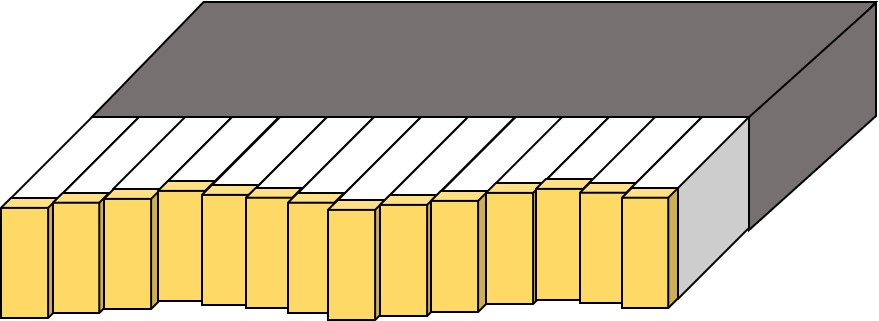
\includegraphics[width=10cm]{images/Wave_Maker(Snake).jpg}
    \caption{3-dimensional wavemaker(snake-like)}
    \label{Snake Wave Maker}
\end{figure}

In other words, the 3-dimensional wavemaker is needed. Though it's not 3-dimensional, the signal provided to the motor could be modified. In a special case, a tsunami could be generated \cite{watts1998wavemaker}.
 
 % 결론
	
	%\clearpage  %%% Appendix를 새 페이지에서 시작
\appendix
\renewcommand{\thesection}{\Alph{section}} %%% TOC에 appendix numbering 재설정
\renewcommand{\thesubsection}{\arabic{subsection}}
\renewcommand{\thesubsubsection}{\arabic{subsubsection}}
\titleformat{\section}[hang] {\normalfont\fontsize{21}{21}\selectfont\bfseries}{\Alph{section}.}{1em}{} %%% Appendix section title의 재설정
\titleformat{\subsection}[hang] {\normalfont\fontsize{16}{16}\selectfont\bfseries}{\Alph{section}.\arabic{subsection}.}{1em}{}
\titleformat{\subsubsection}[hang] {\normalfont\fontsize{14}{14}\selectfont}{\Alph{section}.\arabic{subsection}.\arabic{subsubsection}.}{1em}{}
\titleformat{\paragraph}[hang] {\normalfont\fontsize{12}{12}\selectfont\it}{}{1em}{}
\renewcommand{\theequation}{\thesection.\arabic{equation}} %%% Appendix equation numbering 의 재설정
\renewcommand{\thefigure}{\thesection-\arabic{figure}} %%% Appendix figure numbering 의 재설정
\renewcommand{\thetable}{\thesection-\arabic{table}} %%% Appendix table numbering 의 재설정
\setcounter{equation}{0} %%% Appendix equation starting number의 초기화
\setcounter{figure}{0} %%% Appendix figure starting number의 초기화
\setcounter{table}{0} %%% Appendix table starting number의 초기화


\section{Arduino Code for Wave Maker}

% \subsection*{main.ino}
\lstinputlisting[language=c++]{wavemaker/a_pagefunc.ino}
\lstinputlisting[language=c++]{wavemaker/b_button.ino}
\lstinputlisting[language=c++]{wavemaker/c_move.ino}
\lstinputlisting[language=c++]{wavemaker/d_menu.ino}
\lstinputlisting[language=c++]{wavemaker/menu.ino}
\lstinputlisting[language=c++]{wavemaker/sin_wave.ino}

\section{Experiment Data}
\begin{quote}
    \textbf{Notice}: Graphs of the plate displacement and wave height over time were provided below. Units were omitted, which were $\mathrm{~rad/s}$ and $\mathrm{~cm}$ for $\omega$ and $A$, respectively. Out of the conditions given in the Method section, the following cases were omitted: $(\omega, ~A) = (3, 6), (3, 7), (3, 8), (3, 9), (3, 10), (4, 8), (4, 9), (4, 10)$

    Analyzing the data at such a low $\omega$ was meaningless since external noise was not negligible. Also, the motor moved unexpectedly with the cases of $\omega=4$ above, and they were not analyzed.
\end{quote}

\subsection{Plate movement}
\begin{figure}[H]
\begin{center}
\begin{tabular}{cc}
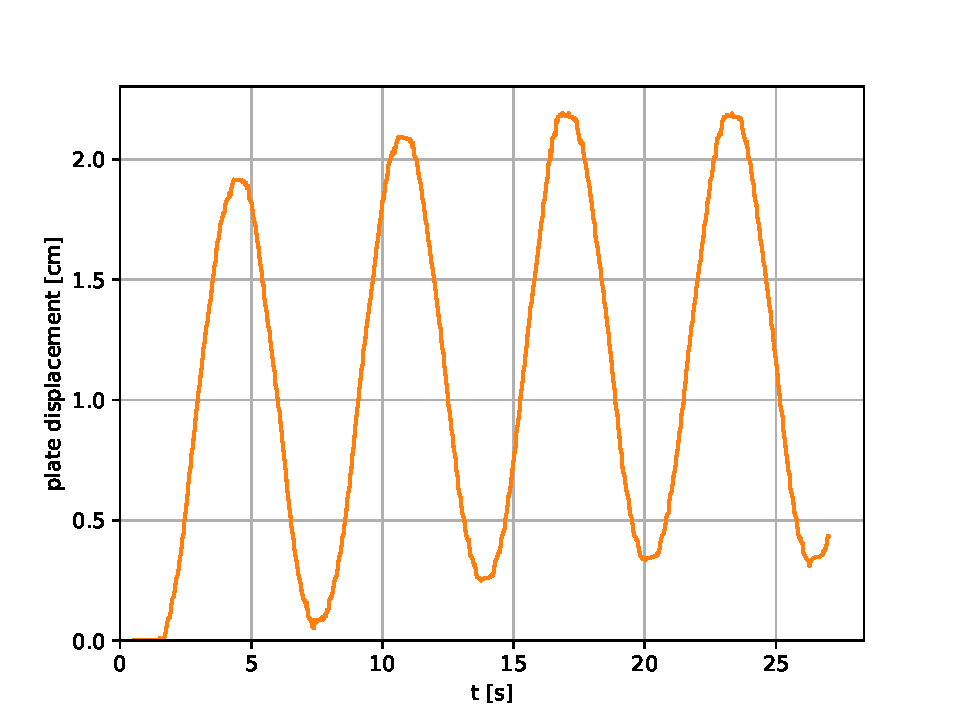
\includegraphics[width=0.45\textwidth, height=3.5cm]{graph/omega=0.50_A=1_plate.pdf}
&
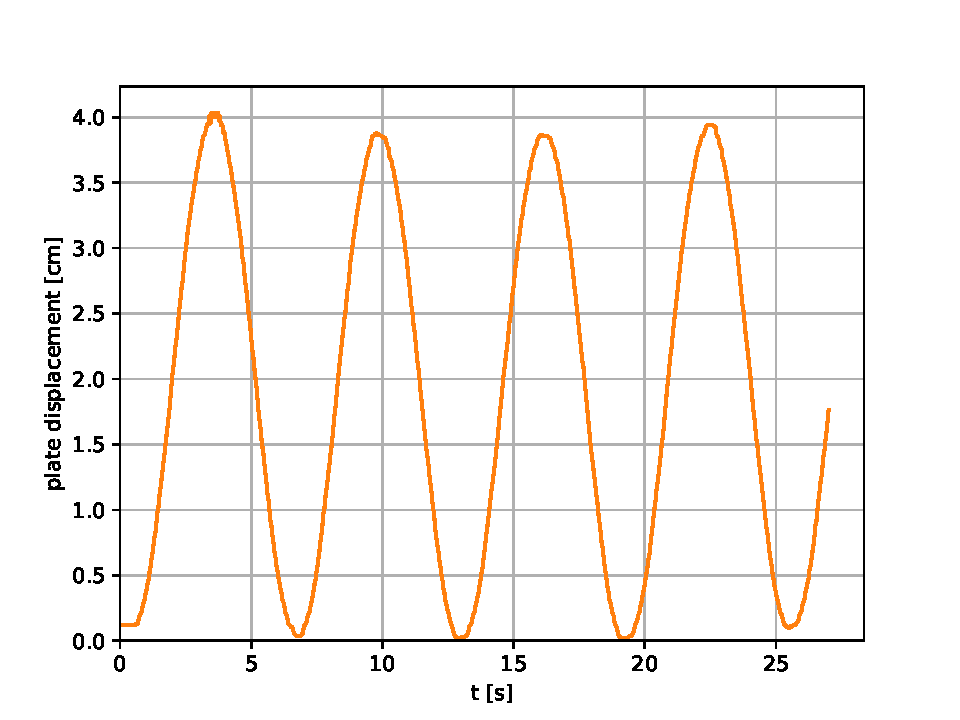
\includegraphics[width=0.45\textwidth, height=3.5cm]{graph/omega=0.50_A=2_plate.pdf}\\
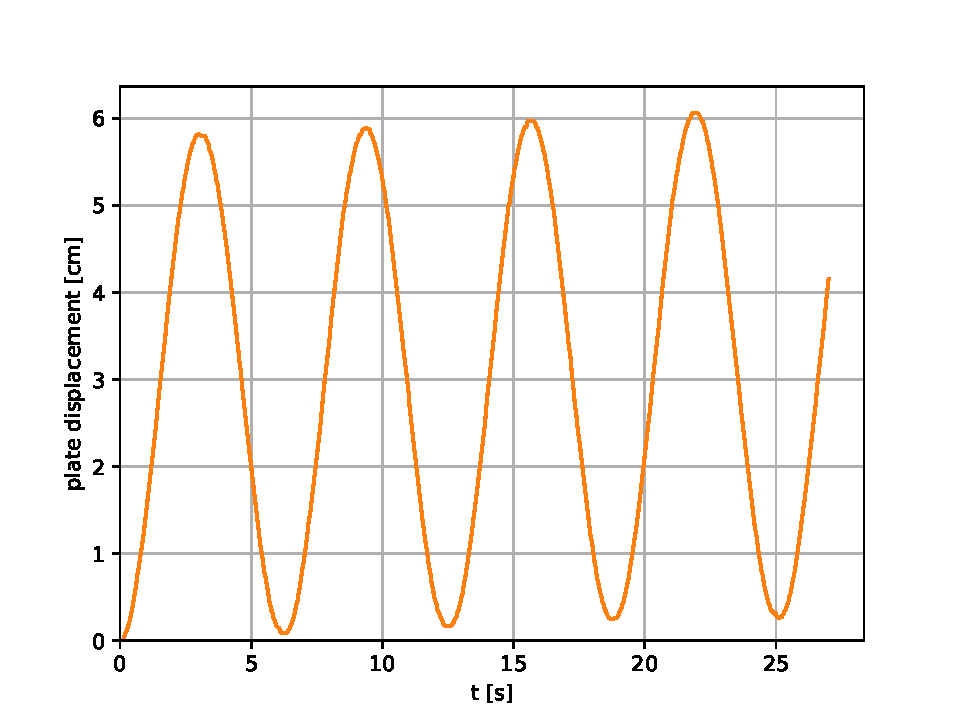
\includegraphics[width=0.45\textwidth, height=3.5cm]{graph/omega=0.50_A=3_plate.pdf}
&
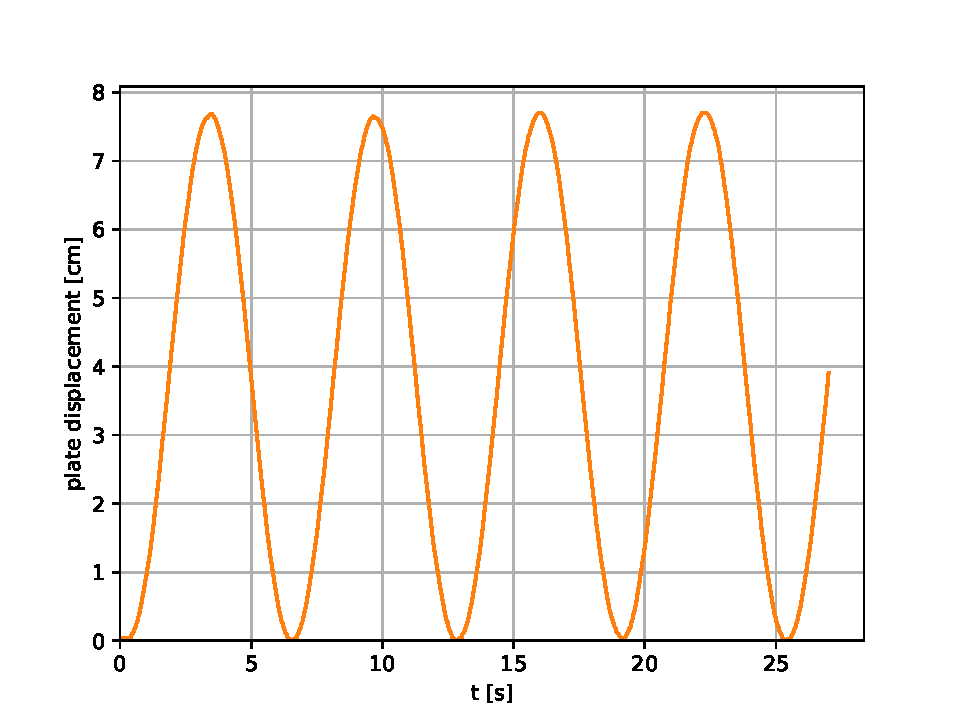
\includegraphics[width=0.45\textwidth, height=3.5cm]{graph/omega=0.50_A=4_plate.pdf}\\
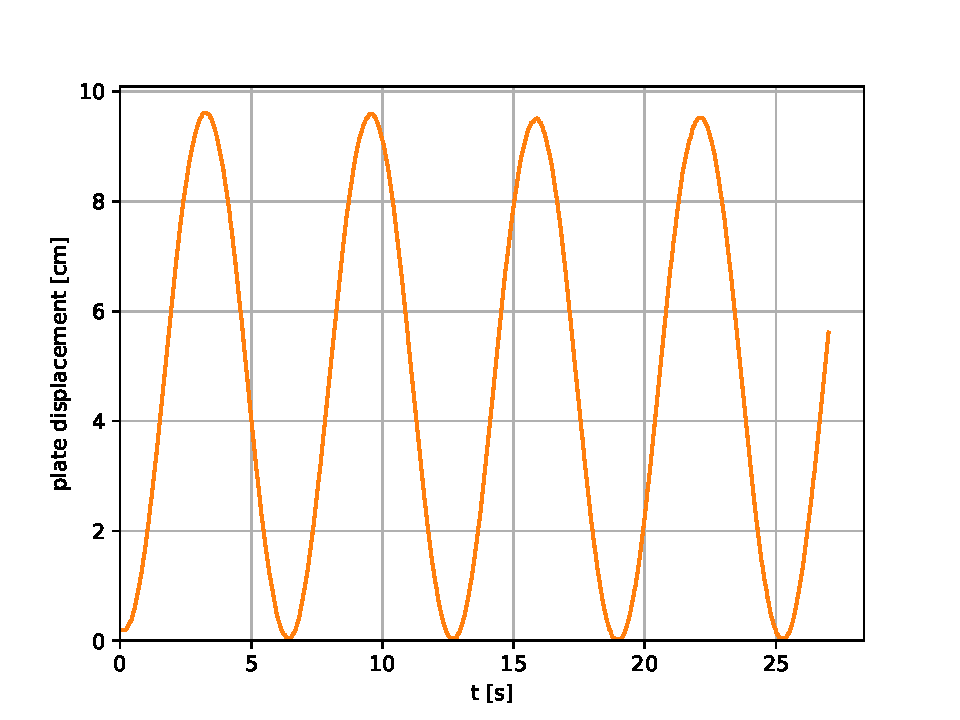
\includegraphics[width=0.45\textwidth, height=3.5cm]{graph/omega=0.50_A=5_plate.pdf}
&
\\
&
\\
&
\\
\end{tabular}
\end{center}
\begin{tikzpicture} [remember picture, overlay]
\node at (3.9, 8.7) {(a)};
\node at (10.8, 8.7) {(b)};
\node at (3.9, 5.0) {(c)};
\node at (10.8, 5.0) {(d)};
\node at (3.9, 1.4) {(e)};
\end{tikzpicture}
\caption{Plate movement - $\omega=3$ \\ (a) $A=1\mathrm{~cm}$ (b) $A=2\mathrm{~cm}$ (c) $A=3\mathrm{~cm}$ (d) $A=4\mathrm{~cm}$ (e) $A=5\mathrm{~cm}$\\(f) $A=6\mathrm{~cm}$ (g) $A=7\mathrm{~cm}$ (h) $A=8\mathrm{~cm}$ (i) $A=9\mathrm{~cm}$ (j) $A=10\mathrm{~cm}$}
\label{Data_omega=3_plate}
\end{figure}

\begin{figure}[H]
\begin{center}
\begin{tabular}{cc}
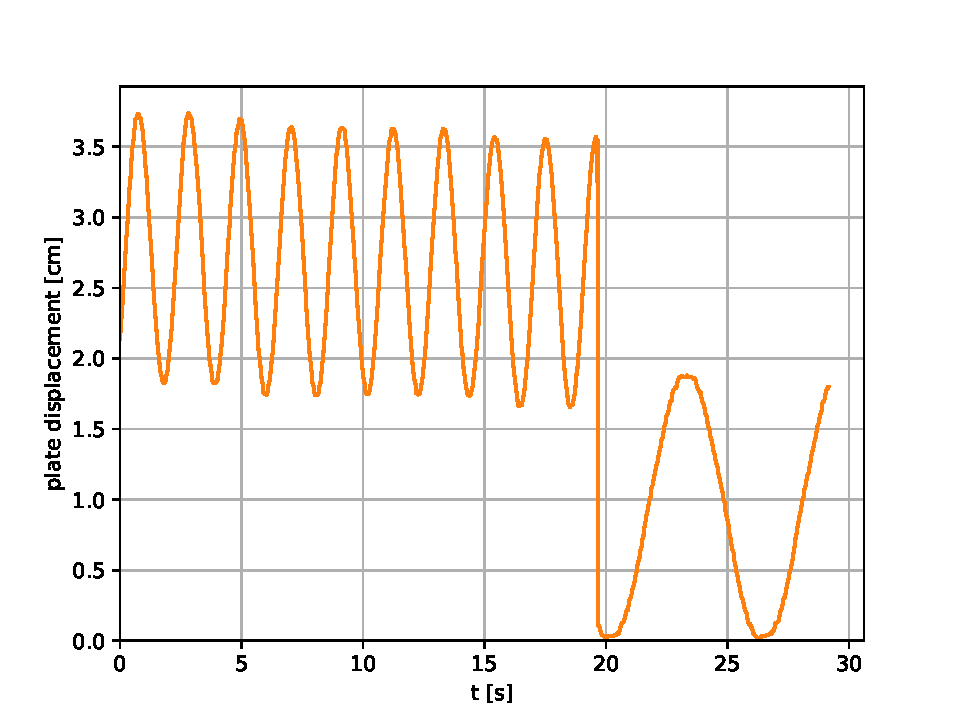
\includegraphics[width=0.45\textwidth, height=3.5cm]{graph/omega=1.00_A=1_plate.pdf}
&
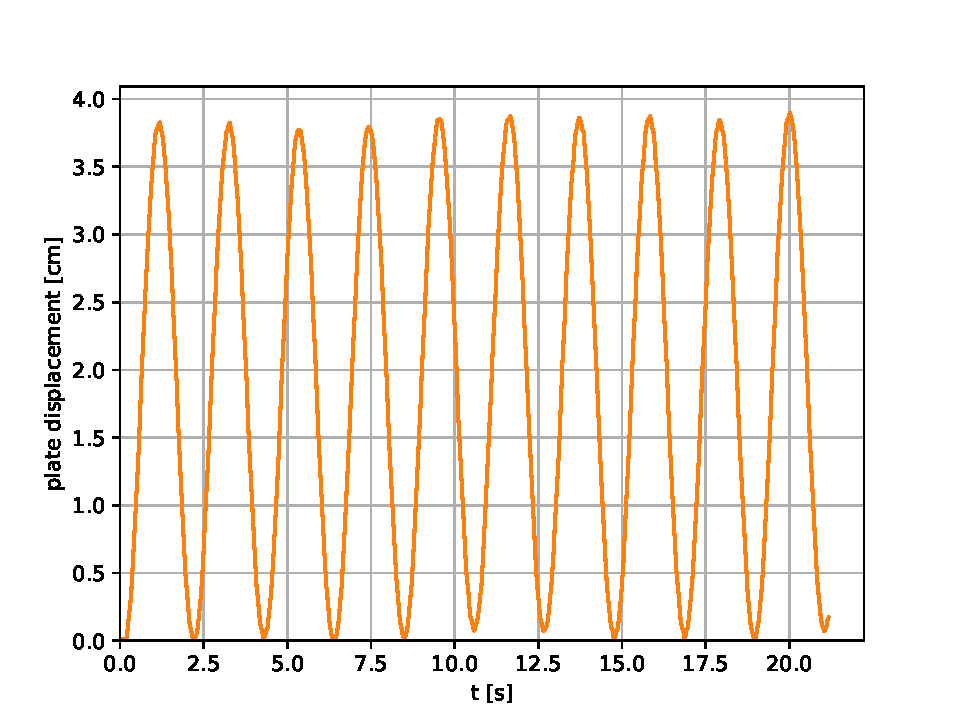
\includegraphics[width=0.45\textwidth, height=3.5cm]{graph/omega=1.00_A=2_plate.pdf}\\
\includegraphics[width=0.45\textwidth, height=3.5cm]{graph/omega=1.00_A=3_plate.pdf}
&
\includegraphics[width=0.45\textwidth, height=3.5cm]{graph/omega=1.00_A=4_plate.pdf}\\
\includegraphics[width=0.45\textwidth, height=3.5cm]{graph/omega=1.00_A=5_plate.pdf}
&
\includegraphics[width=0.45\textwidth, height=3.5cm]{graph/omega=1.00_A=6_plate.pdf}\\
\includegraphics[width=0.45\textwidth, height=3.5cm]{graph/omega=1.00_A=7_plate.pdf}
&
\\
&
\\
\end{tabular}
\end{center}
\begin{tikzpicture} [remember picture, overlay]
\node at (3.9, 11.8) {(a)};
\node at (10.8, 11.8) {(b)};
\node at (3.9, 8.2) {(c)};
\node at (10.8, 8.2) {(d)};
\node at (3.9, 4.5) {(e)};
\node at (10.8, 4.5) {(f)};
\node at (3.9, 0.9) {(g)};
\end{tikzpicture}
\caption{Plate movement - $\omega=4$ \\ (a) $A=1\mathrm{~cm}$ (b) $A=2\mathrm{~cm}$ (c) $A=3\mathrm{~cm}$ (d) $A=4\mathrm{~cm}$ (e) $A=5\mathrm{~cm}$\\(f) $A=6\mathrm{~cm}$ (g) $A=7\mathrm{~cm}$ (h) $A=8\mathrm{~cm}$ (i) $A=9\mathrm{~cm}$ (j) $A=10\mathrm{~cm}$}
\label{Data_omega=4_plate}
\end{figure}

\begin{figure}[H]
\begin{center}
\begin{tabular}{cc}
\includegraphics[width=0.45\textwidth, height=3.5cm]{graph/omega=1.50_A=1_plate.pdf}
&
\includegraphics[width=0.45\textwidth, height=3.5cm]{graph/omega=1.50_A=2_plate.pdf}\\
\includegraphics[width=0.45\textwidth, height=3.5cm]{graph/omega=1.50_A=3_plate.pdf}
&
\includegraphics[width=0.45\textwidth, height=3.5cm]{graph/omega=1.50_A=4_plate.pdf}\\
\includegraphics[width=0.45\textwidth, height=3.5cm]{graph/omega=1.50_A=5_plate.pdf}
&
\includegraphics[width=0.45\textwidth, height=3.5cm]{graph/omega=1.50_A=6_plate.pdf}\\
\includegraphics[width=0.45\textwidth, height=3.5cm]{graph/omega=1.50_A=7_plate.pdf}
&
\includegraphics[width=0.45\textwidth, height=3.5cm]{graph/omega=1.50_A=8_plate.pdf}\\
\includegraphics[width=0.45\textwidth, height=3.5cm]{graph/omega=1.50_A=9_plate.pdf}
&
\includegraphics[width=0.45\textwidth, height=3.5cm]{graph/omega=1.50_A=10_plate.pdf}\\
\end{tabular}
\end{center}
\begin{tikzpicture} [remember picture, overlay]
\node at (3.9, 15.0) {(a)};
\node at (10.8, 15.0) {(b)};
\node at (3.9, 11.4) {(c)};
\node at (10.8, 11.4) {(d)};
\node at (3.9, 7.7) {(e)};
\node at (10.8, 7.7) {(f)};
\node at (3.9, 4.1) {(g)};
\node at (10.8, 4.1) {(h)};
\node at (3.9, 0.4) {(i)};
\node at (10.8, 0.4) {(j)};
\end{tikzpicture}
\caption{Plate movement - $\omega=6$ \\ (a) $A=1\mathrm{~cm}$ (b) $A=2\mathrm{~cm}$ (c) $A=3\mathrm{~cm}$ (d) $A=4\mathrm{~cm}$ (e) $A=5\mathrm{~cm}$\\(f) $A=6\mathrm{~cm}$ (g) $A=7\mathrm{~cm}$ (h) $A=8\mathrm{~cm}$ (i) $A=9\mathrm{~cm}$ (j) $A=10\mathrm{~cm}$}
\label{Data_omega=6_plate}
\end{figure}

\begin{figure}[H]
\begin{center}
\begin{tabular}{cc}
\includegraphics[width=0.45\textwidth, height=3.5cm]{graph/omega=2.00_A=1_plate.pdf}
&
\includegraphics[width=0.45\textwidth, height=3.5cm]{graph/omega=2.00_A=2_plate.pdf}\\
\includegraphics[width=0.45\textwidth, height=3.5cm]{graph/omega=2.00_A=3_plate.pdf}
&
\includegraphics[width=0.45\textwidth, height=3.5cm]{graph/omega=2.00_A=4_plate.pdf}\\
\includegraphics[width=0.45\textwidth, height=3.5cm]{graph/omega=2.00_A=5_plate.pdf}
&
\includegraphics[width=0.45\textwidth, height=3.5cm]{graph/omega=2.00_A=6_plate.pdf}\\
\includegraphics[width=0.45\textwidth, height=3.5cm]{graph/omega=2.00_A=7_plate.pdf}
&
\includegraphics[width=0.45\textwidth, height=3.5cm]{graph/omega=2.00_A=8_plate.pdf}\\
\includegraphics[width=0.45\textwidth, height=3.5cm]{graph/omega=2.00_A=9_plate.pdf}
&
\includegraphics[width=0.45\textwidth, height=3.5cm]{graph/omega=2.00_A=10_plate.pdf}\\
\end{tabular}
\end{center}
\begin{tikzpicture} [remember picture, overlay]
\node at (3.9, 15.0) {(a)};
\node at (10.8, 15.0) {(b)};
\node at (3.9, 11.4) {(c)};
\node at (10.8, 11.4) {(d)};
\node at (3.9, 7.7) {(e)};
\node at (10.8, 7.7) {(f)};
\node at (3.9, 4.1) {(g)};
\node at (10.8, 4.1) {(h)};
\node at (3.9, 0.4) {(i)};
\node at (10.8, 0.4) {(j)};
\end{tikzpicture}
\caption{Plate movement - $\omega=7$ \\ (a) $A=1\mathrm{~cm}$ (b) $A=2\mathrm{~cm}$ (c) $A=3\mathrm{~cm}$ (d) $A=4\mathrm{~cm}$ (e) $A=5\mathrm{~cm}$\\(f) $A=6\mathrm{~cm}$ (g) $A=7\mathrm{~cm}$ (h) $A=8\mathrm{~cm}$ (i) $A=9\mathrm{~cm}$ (j) $A=10\mathrm{~cm}$}
\label{Data_omega=7_plate}
\end{figure}

\begin{figure}[H]
\begin{center}
\begin{tabular}{cc}
\includegraphics[width=0.45\textwidth, height=3.5cm]{graph/omega=2.50_A=1_plate.pdf}
&
\includegraphics[width=0.45\textwidth, height=3.5cm]{graph/omega=2.50_A=2_plate.pdf}\\
\includegraphics[width=0.45\textwidth, height=3.5cm]{graph/omega=2.50_A=3_plate.pdf}
&
\includegraphics[width=0.45\textwidth, height=3.5cm]{graph/omega=2.50_A=4_plate.pdf}\\
\includegraphics[width=0.45\textwidth, height=3.5cm]{graph/omega=2.50_A=5_plate.pdf}
&
\includegraphics[width=0.45\textwidth, height=3.5cm]{graph/omega=2.50_A=6_plate.pdf}\\
\includegraphics[width=0.45\textwidth, height=3.5cm]{graph/omega=2.50_A=7_plate.pdf}
&
\includegraphics[width=0.45\textwidth, height=3.5cm]{graph/omega=2.50_A=8_plate.pdf}\\
\includegraphics[width=0.45\textwidth, height=3.5cm]{graph/omega=2.50_A=9_plate.pdf}
&
\includegraphics[width=0.45\textwidth, height=3.5cm]{graph/omega=2.50_A=10_plate.pdf}\\
\end{tabular}
\end{center}
\begin{tikzpicture} [remember picture, overlay]
\node at (3.9, 15.0) {(a)};
\node at (10.8, 15.0) {(b)};
\node at (3.9, 11.4) {(c)};
\node at (10.8, 11.4) {(d)};
\node at (3.9, 7.7) {(e)};
\node at (10.8, 7.7) {(f)};
\node at (3.9, 4.1) {(g)};
\node at (10.8, 4.1) {(h)};
\node at (3.9, 0.4) {(i)};
\node at (10.8, 0.4) {(j)};
\end{tikzpicture}
\caption{Plate movement - $\omega=9$ \\ (a) $A=1\mathrm{~cm}$ (b) $A=2\mathrm{~cm}$ (c) $A=3\mathrm{~cm}$ (d) $A=4\mathrm{~cm}$ (e) $A=5\mathrm{~cm}$\\(f) $A=6\mathrm{~cm}$ (g) $A=7\mathrm{~cm}$ (h) $A=8\mathrm{~cm}$ (i) $A=9\mathrm{~cm}$ (j) $A=10\mathrm{~cm}$}
\label{Data_omega=9_plate}
\end{figure}

\begin{figure}[H]
\begin{center}
\begin{tabular}{cc}
\includegraphics[width=0.45\textwidth, height=3.5cm]{graph/omega=3.00_A=1_plate.pdf}
&
\includegraphics[width=0.45\textwidth, height=3.5cm]{graph/omega=3.00_A=2_plate.pdf}\\
\includegraphics[width=0.45\textwidth, height=3.5cm]{graph/omega=3.00_A=3_plate.pdf}
&
\includegraphics[width=0.45\textwidth, height=3.5cm]{graph/omega=3.00_A=4_plate.pdf}\\
\includegraphics[width=0.45\textwidth, height=3.5cm]{graph/omega=3.00_A=5_plate.pdf}
&
\includegraphics[width=0.45\textwidth, height=3.5cm]{graph/omega=3.00_A=6_plate.pdf}\\
\includegraphics[width=0.45\textwidth, height=3.5cm]{graph/omega=3.00_A=7_plate.pdf}
&
\includegraphics[width=0.45\textwidth, height=3.5cm]{graph/omega=3.00_A=8_plate.pdf}\\
\includegraphics[width=0.45\textwidth, height=3.5cm]{graph/omega=3.00_A=9_plate.pdf}
&
\includegraphics[width=0.45\textwidth, height=3.5cm]{graph/omega=3.00_A=10_plate.pdf}\\
\end{tabular}
\end{center}
\begin{tikzpicture} [remember picture, overlay]
\node at (3.9, 15.0) {(a)};
\node at (10.8, 15.0) {(b)};
\node at (3.9, 11.4) {(c)};
\node at (10.8, 11.4) {(d)};
\node at (3.9, 7.7) {(e)};
\node at (10.8, 7.7) {(f)};
\node at (3.9, 4.1) {(g)};
\node at (10.8, 4.1) {(h)};
\node at (3.9, 0.4) {(i)};
\node at (10.8, 0.4) {(j)};
\end{tikzpicture}
\caption{Plate movement - $\omega=10$ \\ (a) $A=1\mathrm{~cm}$ (b) $A=2\mathrm{~cm}$ (c) $A=3\mathrm{~cm}$ (d) $A=4\mathrm{~cm}$ (e) $A=5\mathrm{~cm}$\\(f) $A=6\mathrm{~cm}$ (g) $A=7\mathrm{~cm}$ (h) $A=8\mathrm{~cm}$ (i) $A=9\mathrm{~cm}$ (j) $A=10\mathrm{~cm}$}
\label{Data_omega=10_plate}
\end{figure}

\begin{figure}[H]
\begin{center}
\begin{tabular}{cc}
\includegraphics[width=0.45\textwidth, height=3.5cm]{graph/omega=3.50_A=1_plate.pdf}
&
\includegraphics[width=0.45\textwidth, height=3.5cm]{graph/omega=3.50_A=2_plate.pdf}\\
\includegraphics[width=0.45\textwidth, height=3.5cm]{graph/omega=3.50_A=3_plate.pdf}
&
\includegraphics[width=0.45\textwidth, height=3.5cm]{graph/omega=3.50_A=4_plate.pdf}\\
\includegraphics[width=0.45\textwidth, height=3.5cm]{graph/omega=3.50_A=5_plate.pdf}
&
\includegraphics[width=0.45\textwidth, height=3.5cm]{graph/omega=3.50_A=6_plate.pdf}\\
\includegraphics[width=0.45\textwidth, height=3.5cm]{graph/omega=3.50_A=7_plate.pdf}
&
\includegraphics[width=0.45\textwidth, height=3.5cm]{graph/omega=3.50_A=8_plate.pdf}\\
\includegraphics[width=0.45\textwidth, height=3.5cm]{graph/omega=3.50_A=9_plate.pdf}
&
\includegraphics[width=0.45\textwidth, height=3.5cm]{graph/omega=3.50_A=10_plate.pdf}\\
\end{tabular}
\end{center}
\begin{tikzpicture} [remember picture, overlay]
\node at (3.9, 15.0) {(a)};
\node at (10.8, 15.0) {(b)};
\node at (3.9, 11.4) {(c)};
\node at (10.8, 11.4) {(d)};
\node at (3.9, 7.7) {(e)};
\node at (10.8, 7.7) {(f)};
\node at (3.9, 4.1) {(g)};
\node at (10.8, 4.1) {(h)};
\node at (3.9, 0.4) {(i)};
\node at (10.8, 0.4) {(j)};
\end{tikzpicture}
\caption{Plate movement - $\omega=12$ \\ (a) $A=1\mathrm{~cm}$ (b) $A=2\mathrm{~cm}$ (c) $A=3\mathrm{~cm}$ (d) $A=4\mathrm{~cm}$ (e) $A=5\mathrm{~cm}$\\(f) $A=6\mathrm{~cm}$ (g) $A=7\mathrm{~cm}$ (h) $A=8\mathrm{~cm}$ (i) $A=9\mathrm{~cm}$ (j) $A=10\mathrm{~cm}$}
\label{Data_omega=12_plate}
\end{figure}

%%%%%%%%%%%%%%%%%%%%%%%%%%%%%%%%%%%%%%%%%%%%%%%%%%%%%%%%%%%%
\subsection{Wave height}

\begin{figure}[H]
\begin{center}
\begin{tabular}{cc}
\includegraphics[width=0.45\textwidth, height=3.5cm]{graph/omega=0.50_A=1_wave.pdf}
&
\includegraphics[width=0.45\textwidth, height=3.5cm]{graph/omega=0.50_A=2_wave.pdf}\\
\includegraphics[width=0.45\textwidth, height=3.5cm]{graph/omega=0.50_A=3_wave.pdf}
&
\includegraphics[width=0.45\textwidth, height=3.5cm]{graph/omega=0.50_A=4_wave.pdf}\\
\includegraphics[width=0.45\textwidth, height=3.5cm]{graph/omega=0.50_A=5_wave.pdf}
&
\\
&
\\
&
\\
\end{tabular}
\end{center}
\begin{tikzpicture} [remember picture, overlay]
\node at (3.9, 8.7) {(a)};
\node at (10.8, 8.7) {(b)};
\node at (3.9, 5.0) {(c)};
\node at (10.8, 5.0) {(d)};
\node at (3.9, 1.4) {(e)};
\end{tikzpicture}
\caption{Wave height - $\omega=3$ \\ (a) $A=1\mathrm{~cm}$ (b) $A=2\mathrm{~cm}$ (c) $A=3\mathrm{~cm}$ (d) $A=4\mathrm{~cm}$ (e) $A=5\mathrm{~cm}$}
\label{Data_omega=3_wave}
\end{figure}

\begin{figure}[H]
\begin{center}
\begin{tabular}{cc}
\includegraphics[width=0.45\textwidth, height=3.5cm]{graph/omega=1.00_A=1_wave.pdf}
&
\includegraphics[width=0.45\textwidth, height=3.5cm]{graph/omega=1.00_A=2_wave.pdf}\\
\includegraphics[width=0.45\textwidth, height=3.5cm]{graph/omega=1.00_A=3_wave.pdf}
&
\includegraphics[width=0.45\textwidth, height=3.5cm]{graph/omega=1.00_A=4_wave.pdf}\\
\includegraphics[width=0.45\textwidth, height=3.5cm]{graph/omega=1.00_A=5_wave.pdf}
&
\includegraphics[width=0.45\textwidth, height=3.5cm]{graph/omega=1.00_A=6_wave.pdf}\\
\includegraphics[width=0.45\textwidth, height=3.5cm]{graph/omega=1.00_A=7_wave.pdf}
&
\\
&
\\
\end{tabular}
\end{center}
\begin{tikzpicture} [remember picture, overlay]
\node at (3.9, 11.8) {(a)};
\node at (10.8, 11.8) {(b)};
\node at (3.9, 8.2) {(c)};
\node at (10.8, 8.2) {(d)};
\node at (3.9, 4.5) {(e)};
\node at (10.8, 4.5) {(f)};
\node at (3.9, 0.9) {(g)};
\end{tikzpicture}
\caption{Wave height - $\omega=4$ \\ (a) $A=1\mathrm{~cm}$ (b) $A=2\mathrm{~cm}$ (c) $A=3\mathrm{~cm}$ (d) $A=4\mathrm{~cm}$ (e) $A=5\mathrm{~cm}$\\ (f) $A=6\mathrm{~cm}$ (g) $A=7\mathrm{~cm}$}
\label{Data_omega=4_wave}
\end{figure}

\begin{figure}[H]
\begin{center}
\begin{tabular}{cc}
\includegraphics[width=0.45\textwidth, height=3.5cm]{graph/omega=1.50_A=1_wave.pdf}
&
\includegraphics[width=0.45\textwidth, height=3.5cm]{graph/omega=1.50_A=2_wave.pdf}\\
\includegraphics[width=0.45\textwidth, height=3.5cm]{graph/omega=1.50_A=3_wave.pdf}
&
\includegraphics[width=0.45\textwidth, height=3.5cm]{graph/omega=1.50_A=4_wave.pdf}\\
\includegraphics[width=0.45\textwidth, height=3.5cm]{graph/omega=1.50_A=5_wave.pdf}
&
\includegraphics[width=0.45\textwidth, height=3.5cm]{graph/omega=1.50_A=6_wave.pdf}\\
\includegraphics[width=0.45\textwidth, height=3.5cm]{graph/omega=1.50_A=7_wave.pdf}
&
\includegraphics[width=0.45\textwidth, height=3.5cm]{graph/omega=1.50_A=8_wave.pdf}\\
\includegraphics[width=0.45\textwidth, height=3.5cm]{graph/omega=1.50_A=9_wave.pdf}
&
\includegraphics[width=0.45\textwidth, height=3.5cm]{graph/omega=1.50_A=10_wave.pdf}\\
\end{tabular}
\end{center}
\begin{tikzpicture} [remember picture, overlay]
\node at (3.9, 15.0) {(a)};
\node at (10.8, 15.0) {(b)};
\node at (3.9, 11.4) {(c)};
\node at (10.8, 11.4) {(d)};
\node at (3.9, 7.7) {(e)};
\node at (10.8, 7.7) {(f)};
\node at (3.9, 4.1) {(g)};
\node at (10.8, 4.1) {(h)};
\node at (3.9, 0.4) {(i)};
\node at (10.8, 0.4) {(j)};
\end{tikzpicture}
\caption{Wave height - $\omega=6$ \\ (a) $A=1\mathrm{~cm}$ (b) $A=2\mathrm{~cm}$ (c) $A=3\mathrm{~cm}$ (d) $A=4\mathrm{~cm}$ (e) $A=5\mathrm{~cm}$\\(f) $A=6\mathrm{~cm}$ (g) $A=7\mathrm{~cm}$ (h) $A=8\mathrm{~cm}$ (i) $A=9\mathrm{~cm}$ (j) $A=10\mathrm{~cm}$}
\label{Data_omega=6_wave}
\end{figure}

\begin{figure}[H]
\begin{center}
\begin{tabular}{cc}
\includegraphics[width=0.45\textwidth, height=3.5cm]{graph/omega=2.00_A=1_wave.pdf}
&
\includegraphics[width=0.45\textwidth, height=3.5cm]{graph/omega=2.00_A=2_wave.pdf}\\
\includegraphics[width=0.45\textwidth, height=3.5cm]{graph/omega=2.00_A=3_wave.pdf}
&
\includegraphics[width=0.45\textwidth, height=3.5cm]{graph/omega=2.00_A=4_wave.pdf}\\
\includegraphics[width=0.45\textwidth, height=3.5cm]{graph/omega=2.00_A=5_wave.pdf}
&
\includegraphics[width=0.45\textwidth, height=3.5cm]{graph/omega=2.00_A=6_wave.pdf}\\
\includegraphics[width=0.45\textwidth, height=3.5cm]{graph/omega=2.00_A=7_wave.pdf}
&
\includegraphics[width=0.45\textwidth, height=3.5cm]{graph/omega=2.00_A=8_wave.pdf}\\
\includegraphics[width=0.45\textwidth, height=3.5cm]{graph/omega=2.00_A=9_wave.pdf}
&
\includegraphics[width=0.45\textwidth, height=3.5cm]{graph/omega=2.00_A=10_wave.pdf}\\
\end{tabular}
\end{center}
\begin{tikzpicture} [remember picture, overlay]
\node at (3.9, 15.0) {(a)};
\node at (10.8, 15.0) {(b)};
\node at (3.9, 11.4) {(c)};
\node at (10.8, 11.4) {(d)};
\node at (3.9, 7.7) {(e)};
\node at (10.8, 7.7) {(f)};
\node at (3.9, 4.1) {(g)};
\node at (10.8, 4.1) {(h)};
\node at (3.9, 0.4) {(i)};
\node at (10.8, 0.4) {(j)};
\end{tikzpicture}
\caption{Wave height - $\omega=7$ \\ (a) $A=1\mathrm{~cm}$ (b) $A=2\mathrm{~cm}$ (c) $A=3\mathrm{~cm}$ (d) $A=4\mathrm{~cm}$ (e) $A=5\mathrm{~cm}$\\(f) $A=6\mathrm{~cm}$ (g) $A=7\mathrm{~cm}$ (h) $A=8\mathrm{~cm}$ (i) $A=9\mathrm{~cm}$ (j) $A=10\mathrm{~cm}$}
\label{Data_omega=7_wave}
\end{figure}

\begin{figure}[H]
\begin{center}
\begin{tabular}{cc}
\includegraphics[width=0.45\textwidth, height=3.5cm]{graph/omega=2.50_A=1_wave.pdf}
&
\includegraphics[width=0.45\textwidth, height=3.5cm]{graph/omega=2.50_A=2_wave.pdf}\\
\includegraphics[width=0.45\textwidth, height=3.5cm]{graph/omega=2.50_A=3_wave.pdf}
&
\includegraphics[width=0.45\textwidth, height=3.5cm]{graph/omega=2.50_A=4_wave.pdf}\\
\includegraphics[width=0.45\textwidth, height=3.5cm]{graph/omega=2.50_A=5_wave.pdf}
&
\includegraphics[width=0.45\textwidth, height=3.5cm]{graph/omega=2.50_A=6_wave.pdf}\\
\includegraphics[width=0.45\textwidth, height=3.5cm]{graph/omega=2.50_A=7_wave.pdf}
&
\includegraphics[width=0.45\textwidth, height=3.5cm]{graph/omega=2.50_A=8_wave.pdf}\\
\includegraphics[width=0.45\textwidth, height=3.5cm]{graph/omega=2.50_A=9_wave.pdf}
&
\includegraphics[width=0.45\textwidth, height=3.5cm]{graph/omega=2.50_A=10_wave.pdf}\\
\end{tabular}
\end{center}
\begin{tikzpicture} [remember picture, overlay]
\node at (3.9, 15.0) {(a)};
\node at (10.8, 15.0) {(b)};
\node at (3.9, 11.4) {(c)};
\node at (10.8, 11.4) {(d)};
\node at (3.9, 7.7) {(e)};
\node at (10.8, 7.7) {(f)};
\node at (3.9, 4.1) {(g)};
\node at (10.8, 4.1) {(h)};
\node at (3.9, 0.4) {(i)};
\node at (10.8, 0.4) {(j)};
\end{tikzpicture}
\caption{Wave height - $\omega=9$ \\ (a) $A=1\mathrm{~cm}$ (b) $A=2\mathrm{~cm}$ (c) $A=3\mathrm{~cm}$ (d) $A=4\mathrm{~cm}$ (e) $A=5\mathrm{~cm}$\\(f) $A=6\mathrm{~cm}$ (g) $A=7\mathrm{~cm}$ (h) $A=8\mathrm{~cm}$ (i) $A=9\mathrm{~cm}$ (j) $A=10\mathrm{~cm}$}
\label{Data_omega=9_wave}
\end{figure}

\begin{figure}[H]
\begin{center}
\begin{tabular}{cc}
\includegraphics[width=0.45\textwidth, height=3.5cm]{graph/omega=3.00_A=1_wave.pdf}
&
\includegraphics[width=0.45\textwidth, height=3.5cm]{graph/omega=3.00_A=2_wave.pdf}\\
\includegraphics[width=0.45\textwidth, height=3.5cm]{graph/omega=3.00_A=3_wave.pdf}
&
\includegraphics[width=0.45\textwidth, height=3.5cm]{graph/omega=3.00_A=4_wave.pdf}\\
\includegraphics[width=0.45\textwidth, height=3.5cm]{graph/omega=3.00_A=5_wave.pdf}
&
\includegraphics[width=0.45\textwidth, height=3.5cm]{graph/omega=3.00_A=6_wave.pdf}\\
\includegraphics[width=0.45\textwidth, height=3.5cm]{graph/omega=3.00_A=7_wave.pdf}
&
\includegraphics[width=0.45\textwidth, height=3.5cm]{graph/omega=3.00_A=8_wave.pdf}\\
\includegraphics[width=0.45\textwidth, height=3.5cm]{graph/omega=3.00_A=9_wave.pdf}
&
\includegraphics[width=0.45\textwidth, height=3.5cm]{graph/omega=3.00_A=10_wave.pdf}\\
\end{tabular}
\end{center}
\begin{tikzpicture} [remember picture, overlay]
\node at (3.9, 15.0) {(a)};
\node at (10.8, 15.0) {(b)};
\node at (3.9, 11.4) {(c)};
\node at (10.8, 11.4) {(d)};
\node at (3.9, 7.7) {(e)};
\node at (10.8, 7.7) {(f)};
\node at (3.9, 4.1) {(g)};
\node at (10.8, 4.1) {(h)};
\node at (3.9, 0.4) {(i)};
\node at (10.8, 0.4) {(j)};
\end{tikzpicture}
\caption{Wave height - $\omega=10$ \\ (a) $A=1\mathrm{~cm}$ (b) $A=2\mathrm{~cm}$ (c) $A=3\mathrm{~cm}$ (d) $A=4\mathrm{~cm}$ (e) $A=5\mathrm{~cm}$\\(f) $A=6\mathrm{~cm}$ (g) $A=7\mathrm{~cm}$ (h) $A=8\mathrm{~cm}$ (i) $A=9\mathrm{~cm}$ (j) $A=10\mathrm{~cm}$}
\label{Data_omega=10_wave}
\end{figure}

\begin{figure}[H]
\begin{center}
\begin{tabular}{cc}
\includegraphics[width=0.45\textwidth, height=3.5cm]{graph/omega=3.50_A=1_wave.pdf}
&
\includegraphics[width=0.45\textwidth, height=3.5cm]{graph/omega=3.50_A=2_wave.pdf}\\
\includegraphics[width=0.45\textwidth, height=3.5cm]{graph/omega=3.50_A=3_wave.pdf}
&
\includegraphics[width=0.45\textwidth, height=3.5cm]{graph/omega=3.50_A=4_wave.pdf}\\
\includegraphics[width=0.45\textwidth, height=3.5cm]{graph/omega=3.50_A=5_wave.pdf}
&
\includegraphics[width=0.45\textwidth, height=3.5cm]{graph/omega=3.50_A=6_wave.pdf}\\
\includegraphics[width=0.45\textwidth, height=3.5cm]{graph/omega=3.50_A=7_wave.pdf}
&
\includegraphics[width=0.45\textwidth, height=3.5cm]{graph/omega=3.50_A=8_wave.pdf}\\
\includegraphics[width=0.45\textwidth, height=3.5cm]{graph/omega=3.50_A=9_wave.pdf}
&
\includegraphics[width=0.45\textwidth, height=3.5cm]{graph/omega=3.50_A=10_wave.pdf}\\
\end{tabular}
\end{center}
\begin{tikzpicture} [remember picture, overlay]
\node at (3.9, 15.0) {(a)};
\node at (10.8, 15.0) {(b)};
\node at (3.9, 11.4) {(c)};
\node at (10.8, 11.4) {(d)};
\node at (3.9, 7.7) {(e)};
\node at (10.8, 7.7) {(f)};
\node at (3.9, 4.1) {(g)};
\node at (10.8, 4.1) {(h)};
\node at (3.9, 0.4) {(i)};
\node at (10.8, 0.4) {(j)};
\end{tikzpicture}
\caption{Wave height - $\omega=12$ \\ (a) $A=1\mathrm{~cm}$ (b) $A=2\mathrm{~cm}$ (c) $A=3\mathrm{~cm}$ (d) $A=4\mathrm{~cm}$ (e) $A=5\mathrm{~cm}$\\(f) $A=6\mathrm{~cm}$ (g) $A=7\mathrm{~cm}$ (h) $A=8\mathrm{~cm}$ (i) $A=9\mathrm{~cm}$ (j) $A=10\mathrm{~cm}$}
\label{Data_omega=12_wave}
\end{figure} % 부록(없으면 주석 처리)
	
	\bibliography{bibfile} % 참고문헌
	% BibTeX 코드 쉽게 얻어오는 방법 %
	% Google Scholar 에서 검색한 결과에서 `인용'을 클릭한다.
	% BibTeX 코드를 얻고자 한다면, 하단의 `BibTeX' 을 클릭.
	% 코드가 나온다. Ctrl+A, Ctrl+C로 복사, bibfile에 붙여넣기.
	
	\include{sub/summary} % 요약
	% 한글로 작성한 학생은 이 부분을 주석 처리하십시오.
	% 영어로 작성할 경우 5페이지 이내의 한글 요약을 작성해야 합니다. (37기 기준)
	
	%-----------------------------------------------------
%   감사의 글
%-----------------------------------------------------
\begin{acknowledgements}
\addcontentsline{toc}{section}{Acknowledgements}  %%% TOC에 표시
    
    % First and foremost, I would like to thank my research supervisor, Kihyuen Park. Without his assistance and dedication, this paper couldn't be accomplished. He helped me handle electronic devices, design circuits, and PCB, give ideas for our experimenting system, and even write documents with \LaTeX. I would like to thank him very much for his great support over the past year. Also, I would like to appreciate Youngjoon Jeon, an advisor to the research for comparing the masonry structure of the breakwater and making a proper environment for it in 2021. From this research, he made a wave channel with a length of $4,000\mathrm{~mm}$, the one already built before this research. If it had not been for him and his hard work, this research could not have gotten started.

    % I would also like to show gratitude to my consultant, professor Sungwon Shin at ERICA Campus, Hanyang University. He advised us and introduced the basic concept of coastal engineering. Also, he had invited our team to his lab, and even came to our lab himself, giving out feedback on our experimenting system. The basic design of our devices was motivated by his lab, and he willingly let us do so, plus introducing related studies and experiments.
    

    % During the whole research, I had my teammates, Hyosong Baek, and Sihyun Lee, who communicated and solved problems altogether. Sihyeon helped to make wave absorbers and a wave gauge. She didn't resist giving out ideas when we faced many structural problems, and most of the ideas eventually worked out finely. Hyosong is our best programmer, coding most of the commands for our Wavemaker's, software. There had been a lot of problems with various parameters, and she discovered what \textit{MaxSpeed} and \textit{MaxAcceleration} do, and how those parameters eventually affect the signal. \textit{Code Test} involves a lot more trial and error, and Hyosong was the one who was in charge of it. She connected a button to the circuit so that it works as a remote control, and is currently working on its manual.

    % Though not every moment was hopeful and successful and even sometimes, our wave maker failed to work, I could keep on the research because so many people gave their hands to me. They tried to give ideas, hope, and confidence. I feel grateful for all of them.

    First and foremost, I extend my deepest appreciation to my research supervisor, Kihyuen Park, whose exceptional guidance and unwavering dedication have been pivotal to the successful completion of this paper. His expertise encompassed various aspects, including the handling of electronic devices, circuit and PCB design, the conceptualization of the experimenting system, and proficiency in document preparation using \LaTeX. I am sincerely grateful for his invaluable support throughout the past year.

    I would also like to acknowledge the invaluable contributions of Youngjoon Jeon, an advisor to this research, who played a crucial role in comparing the masonry structure of the breakwater and establishing an optimal experimental environment in 2021. Through his diligent efforts, a wave channel measuring 4,000 mm in length was constructed, providing a solid foundation for this research. Without his hard work and dedication, this research endeavor would not have been initiated.

    Additionally, I am indebted to Professor Sungwon Shin, my consultant at ERICA Campus, Hanyang University, for his expert guidance and introduction to the fundamental concepts of coastal engineering. Professor Shin graciously welcomed our team into his laboratory, provided invaluable feedback on our experimenting system, and shared relevant studies and experiments. The basic design of our devices drew inspiration from his laboratory, and his unwavering support allowed us to proceed with our research.

    Throughout the entire research process, I was fortunate to have the collaboration and support of my teammates, Hyosong Baek and Sihyun Lee, who greatly contributed to effective communication and joint problem-solving. Sihyeon played a crucial role in constructing wave absorbers and wave gauges. Her proactive approach to offering ideas to overcome numerous structural challenges proved highly effective. Hyosong, our skilled programmer, demonstrated exceptional coding proficiency in developing the software for our wavemaker. In the face of various parameter-related challenges, she successfully deciphered the functions and implications of critical parameters such as \textit{MaxSpeed} and \textit{MaxAcceleration}, ultimately influencing the signal quality. The \textit{Code Test} phase involved extensive trial and error, for which Hyosong assumed responsibility. Additionally, she incorporated a remote control functionality by integrating a button into the circuit, and she is currently working on its manual.

    While not every moment of this research journey was marked by success and optimism, and despite occasional setbacks where our wavemaker failed to operate as intended, I was able to persevere due to the generous support of numerous individuals. Their continuous provision of ideas, hope, and confidence greatly uplifted my spirits, for which I am deeply grateful.
    
\end{acknowledgements}

%-----------------------------------------------------
%   연구활동 
%-----------------------------------------------------
\begin{researches}
% \addcontentsline{toc}{section}{연구활동}  %%% TOC에 표시
% \begin{itemize}
% \item{2011학년도 교내 R\&E 발표대회에서 장려상 수상}
% \item{2012학년도 교내 R\&E 발표대회에서 장려상 수상}
% \item{2013학년도 교내 R\&E 발표대회에서 장려상 수상}
% \item{2014학년도 교내 R\&E 발표대회에서 장려상 수상}
% \item{2015학년도 교내 R\&E 발표대회에서 장려상 수상}
% \item{2016학년도 교내 R\&E 발표대회에서 장려상 수상}
% \item{2017학년도 교내 R\&E 발표대회에서 장려상 수상}
% \item{2018학년도 교내 R\&E 발표대회에서 장려상 수상}
% \item{2019년 노벨 물리학상 수상}
% \end{itemize}

\addcontentsline{toc}{section}{Perfomance of the Research}  %%% TOC에 표시
\begin{itemize}
\item{2022학년도 추계 지구과학학술대회에서 장려상 수상}
\end{itemize}
\end{researches} % 감사의 글 & 연구활동
        % \section{구두발표}
\begin{quote}
    \begin{center}
    \textbf{지구과학과 졸업논문 구두발표 안내}
        \begin{itemize}
            \item 일시 : 3/27(월) 16:50~18:40 (10분/1인)
            \item 장소: SRC629
            \item 발표자료 :  슬라이드 또는 작성하고 있는 논문
            \item 포함해야 할 내용: 졸업 논문 진행 상황 및 완성 계획
            \item 시간 엄수: 발표시간 7분, 질의응답 3분
        \end{itemize}
            
        성실하게 준비해서 발표하시고, 미비하면 구두발표를 다시 해야 함.
    \end{center}
\end{quote}

\subsection{현황}
\begin{itemize}
    \item \textbf{초록, 감사의 말, 부록, 요약}\\
    마지막에 작성할 예정 (그렇지만 계속 염두에 두고 있음)
    
    \item \textbf{서론}\\
    방학동안 조파기 제작 및 WMT 관련 논문을 다수 찾아봄. WMT와 관련된 여러 논문은 찾았으나 연구 동향과 관련된 논문은 찾기가 어려웠고 현재는 1장 반 정도 작성함. 주 내용은 조파기 관련 연구가 어떻게 발전해왔고 우리 연구는 이미 있던 실험장비를 확장시킨 것이라는 식으로 작성함.    

    \item \textbf{이론적 배경}\\
    WMT와 관련한 여러 논문에서 공통적으로 인용하고 있는 논문이 2개가 있음.

    \begin{quote}
        \begin{enumerate}
            \item Dean and Dalrymple
            \item Hughes
        \end{enumerate}
    \end{quote}

    사실 Hughes의 서적이 더 교과서적이지만 문제는 볼 수가 없다는 것. Dean and Dalrymple의 논문은 piston-type wave maker의 부분만 발췌하여 실었으며 이 외에도 여러 논문에서 본 내용을 바탕으로 이론을 전개했으나 지금 쓴 내용으로는 표절률이 상당히 높을 수 있음. 그리고 수식 전개 내용을 다 넣어야 하는지도 의문이긴 함.

    그래서 WMT는 궁극적으로 파고와 관련된 식을 줌. 그리고 추가적으로 조파수조, 조파기, 소파기 및 파고계에 대한 내용도 실음. 파고계는 이번에 창알이 진행되는 정도를 보아 넣을지 말지를 결정할 예정. 넣지 않아도 큰 문제는 없음.

    \item \textbf{연구방법}\\
    여기가 제일 큰 문제임.
    
    \begin{enumerate}
        \item 수조 확장
        \item 조파기 제작 (Hardware 구성)
        \item 조파기 코딩 (SoftWare 구성)
    \end{enumerate}

    겨울방학 동안 진행한 결과는 조파기 코딩에 멈춰있음. 그래도 최근에는 돌파구를 찾아서 잘 되었으면 좋겠지만 이것도 안 된다고 하면 조파기를 완전히 새로 만들 필요가 있음...

    정말 이 상황은 피하고 싶고 sin형 구동이 된다고 하면 파가 생기는 것을 영상을 찍어 분석할 예정. 분석 방법은 파고계가 잘 작동한다면 적극 활용하겠지만 현재로써는 물에 물감을 풀어 사용하는 것이 그나마 최선임. 그리고 이것도 하나의 모드에 대하여 조파기로부터의 거리에 따라서 실험을 해볼 예정.

    조파기 코딩의 확장으로 디스플레이를 이용한 컨트롤러 완성은 정말정말 이상적으로 모든 실험이 끝난 경우에나 할 수 있을 것 같음. 현재 3D 디자인과 기본 구조는 어느정도 잡혀있으나 이걸 진행할 여유가 없음.

    그리고 조파기가 제대로 작동한다면 컨트롤러 완비와 더불어 연안 모형 관련 실험을 진행할 수 있음. 경사로를 어떻게 할지만 생각해놓으면 저번에 관찰한 쇄파 실험을 할 수도 있고 방파제 조적구조 비교 실험을 간단하게 진행할 수도 있음.

    \textbf{사실 이 모든 것은 이미 작년에도 알고 있던 것이며 조파기가 제대로 작동하면 무엇이든 할 수 있다!}    

    \item \textbf{실험결과 및 결론}
    원래 여기에 예비 실험으로 Arduino에서 모터의 각변위를 출력하여 이런 식으로 움직인다는 것을 보이려고 했으나 문제는 출력되는 값이랑 실제 움직이는 거랑 일치하지 않아보일 때가 많음

    Ex) 모터가 탈조가 나서 돌아가지 않아도 값은 계속 출력됨.

    겨울방학 동안 이 데이터들을 좀 뽑아둔 것이 있는데 어차피 작은 모터로 뽑아둔 것이며 보드만 있어도 충분히 가능한 일이기 때문에 큰 의미가 있나 싶음.
    
\end{itemize}

\subsection{앞으로의 계획}
Teensy 4.0이 왔으니까 이거로 조파기가 돌아가기를 기대해야 함. 모든 것이 순탄하다는 가정하에 졸논이나 과전에 넣을 기본적인 sin형 데이터는 1~2주 안으로 다 뽑을 수 있을 듯함.

확실한 것은 중간 전에 거의 다 끝내야 하는데 중간고사가 끝나면 그 굉장히 좋은 시즌에 여러 행사가 겹쳐있기 때문에 그때 모여서 뭔가를 하는 것은 진짜 쉽지 않음. 기껏해야 중간고사가 끝난 날부터 그 주 목, 금에 조금이나마 모일 수 있을 듯함.

\end{document}
